\documentclass{article}
\usepackage{graphicx}
\usepackage{float}
\usepackage{csvsimple}
\usepackage{rotating}
\title{Addendum to ``CHAAHK: A Spatial Simulation Model of the Maya
		Elevated Core Region''}
	\author{Alex Kara}
\begin{document}
\maketitle
\section{Purpose}
In summary, changes from CHAAHK 1.0 to 1.1 include:
\begin{itemize}
	\item Released as an executable installer instead of as an Eclipse project directory.
	\item Improvements to Java code readability and simulation run time.
	\item Redone graphical interface for visual and/or real-time analysis.
	\item Improvements to readability and organization of R scripts.
\end{itemize}
\par In December of 2018 I published version 1.0.0 of the CHAAHK simulation model on the Network for Computational Modeling in Social and Ecological Sciences \cite{kara2018a}. This included a downloadable directory including the model's source code and a large, diverse collection of R-language scripts. These files are basically a time capsule: a perfect representation of the working directory associated with CHAAHK at the time that my thesis was submitted \cite{kara2018b}. Things were not changed from their original state to render my thesis research transparent and reproducible. However, user-friendliness became something of a casualty in the process. Most critically, the uploaded directory was an Eclipse ``project" directory, so the simulation itself could not be easily run without having Eclipse and Repast installed locally. This document accompanies a newer (1.1.0) release of CHAAHK, which comes packaged as an executable installer that only requires Java.
\par In addition, the updates reduced the simulation's execution time, improved the code's readability, and polished the graphical user interface. These considerations were originally low priorities when trying to meet my defense deadline, but are virtually prerequisites to the dissemination and reproduction of CHAAHK or any other social scientific simulation model.  These updates' purpose was to finalize CHAAHK as a deliverable while changing as little about the simulation's actual behavior as possible. They provide a more approachable lens to judge my original thesis for what it's worth. 
\par In addition to cleaning up CHAAHK itself, I also reorganized the many R scripts included with the directory uploaded to CoMSES. Together, they provide all of the R code used to run the simulation, collect output data, and perform the analyses discussed in my thesis. Compared to before, the scripts feature more deliberate variable names, less redundant code, and improved readability. 

\section{Results}
This document illustrates the results of a new series of CHAAHK runs using the updated 1.1.0 implementation. The parameterization of this experiment is identical in terms of sample size and sampling strategy to that presented in my thesis. The same set of output analyses were likewise applied to the results of this experiment. Together, they demonstrate that the results of running the newer CHAAHK implementation are basically the same as those collected from the older implementation scrutinized in my thesis \cite{kara2018b}. Key similarities include 

\begin{itemize}
	\item Only a small number of parameter combinations produce an $ SLG $ less than 0.5. (246 originally, now 276).
	\item $ C_{d}i $ and $ F_{d}i $ are the strongest predictors of model behavior when considering all output data.
	\item However, the distributions of $ C_{d}r $ and $ F_{d}r $ are more skewed than those of the other parameters among runs actually achieving $ SLG  <$  0.5.
\end{itemize}

\section{Conclusion}
There are differences between the original and updated model outputs, but the original synthesis still applies to this newer set of data just the same. I believe this synthesis can be improved through further quantitative analysis. Also, modifying or adding features to CHAAHK itself can improve its value as a model for social evolution in the central Maya Lowlands. CHAAHK 1.1.0 explicitly avoids doing either. However, it is hoped 1.1.0 simply provides more accessible means to scrutinize my masters thesis with all of its original details, for better or for worse, intact.

\begin{figure}[H]
	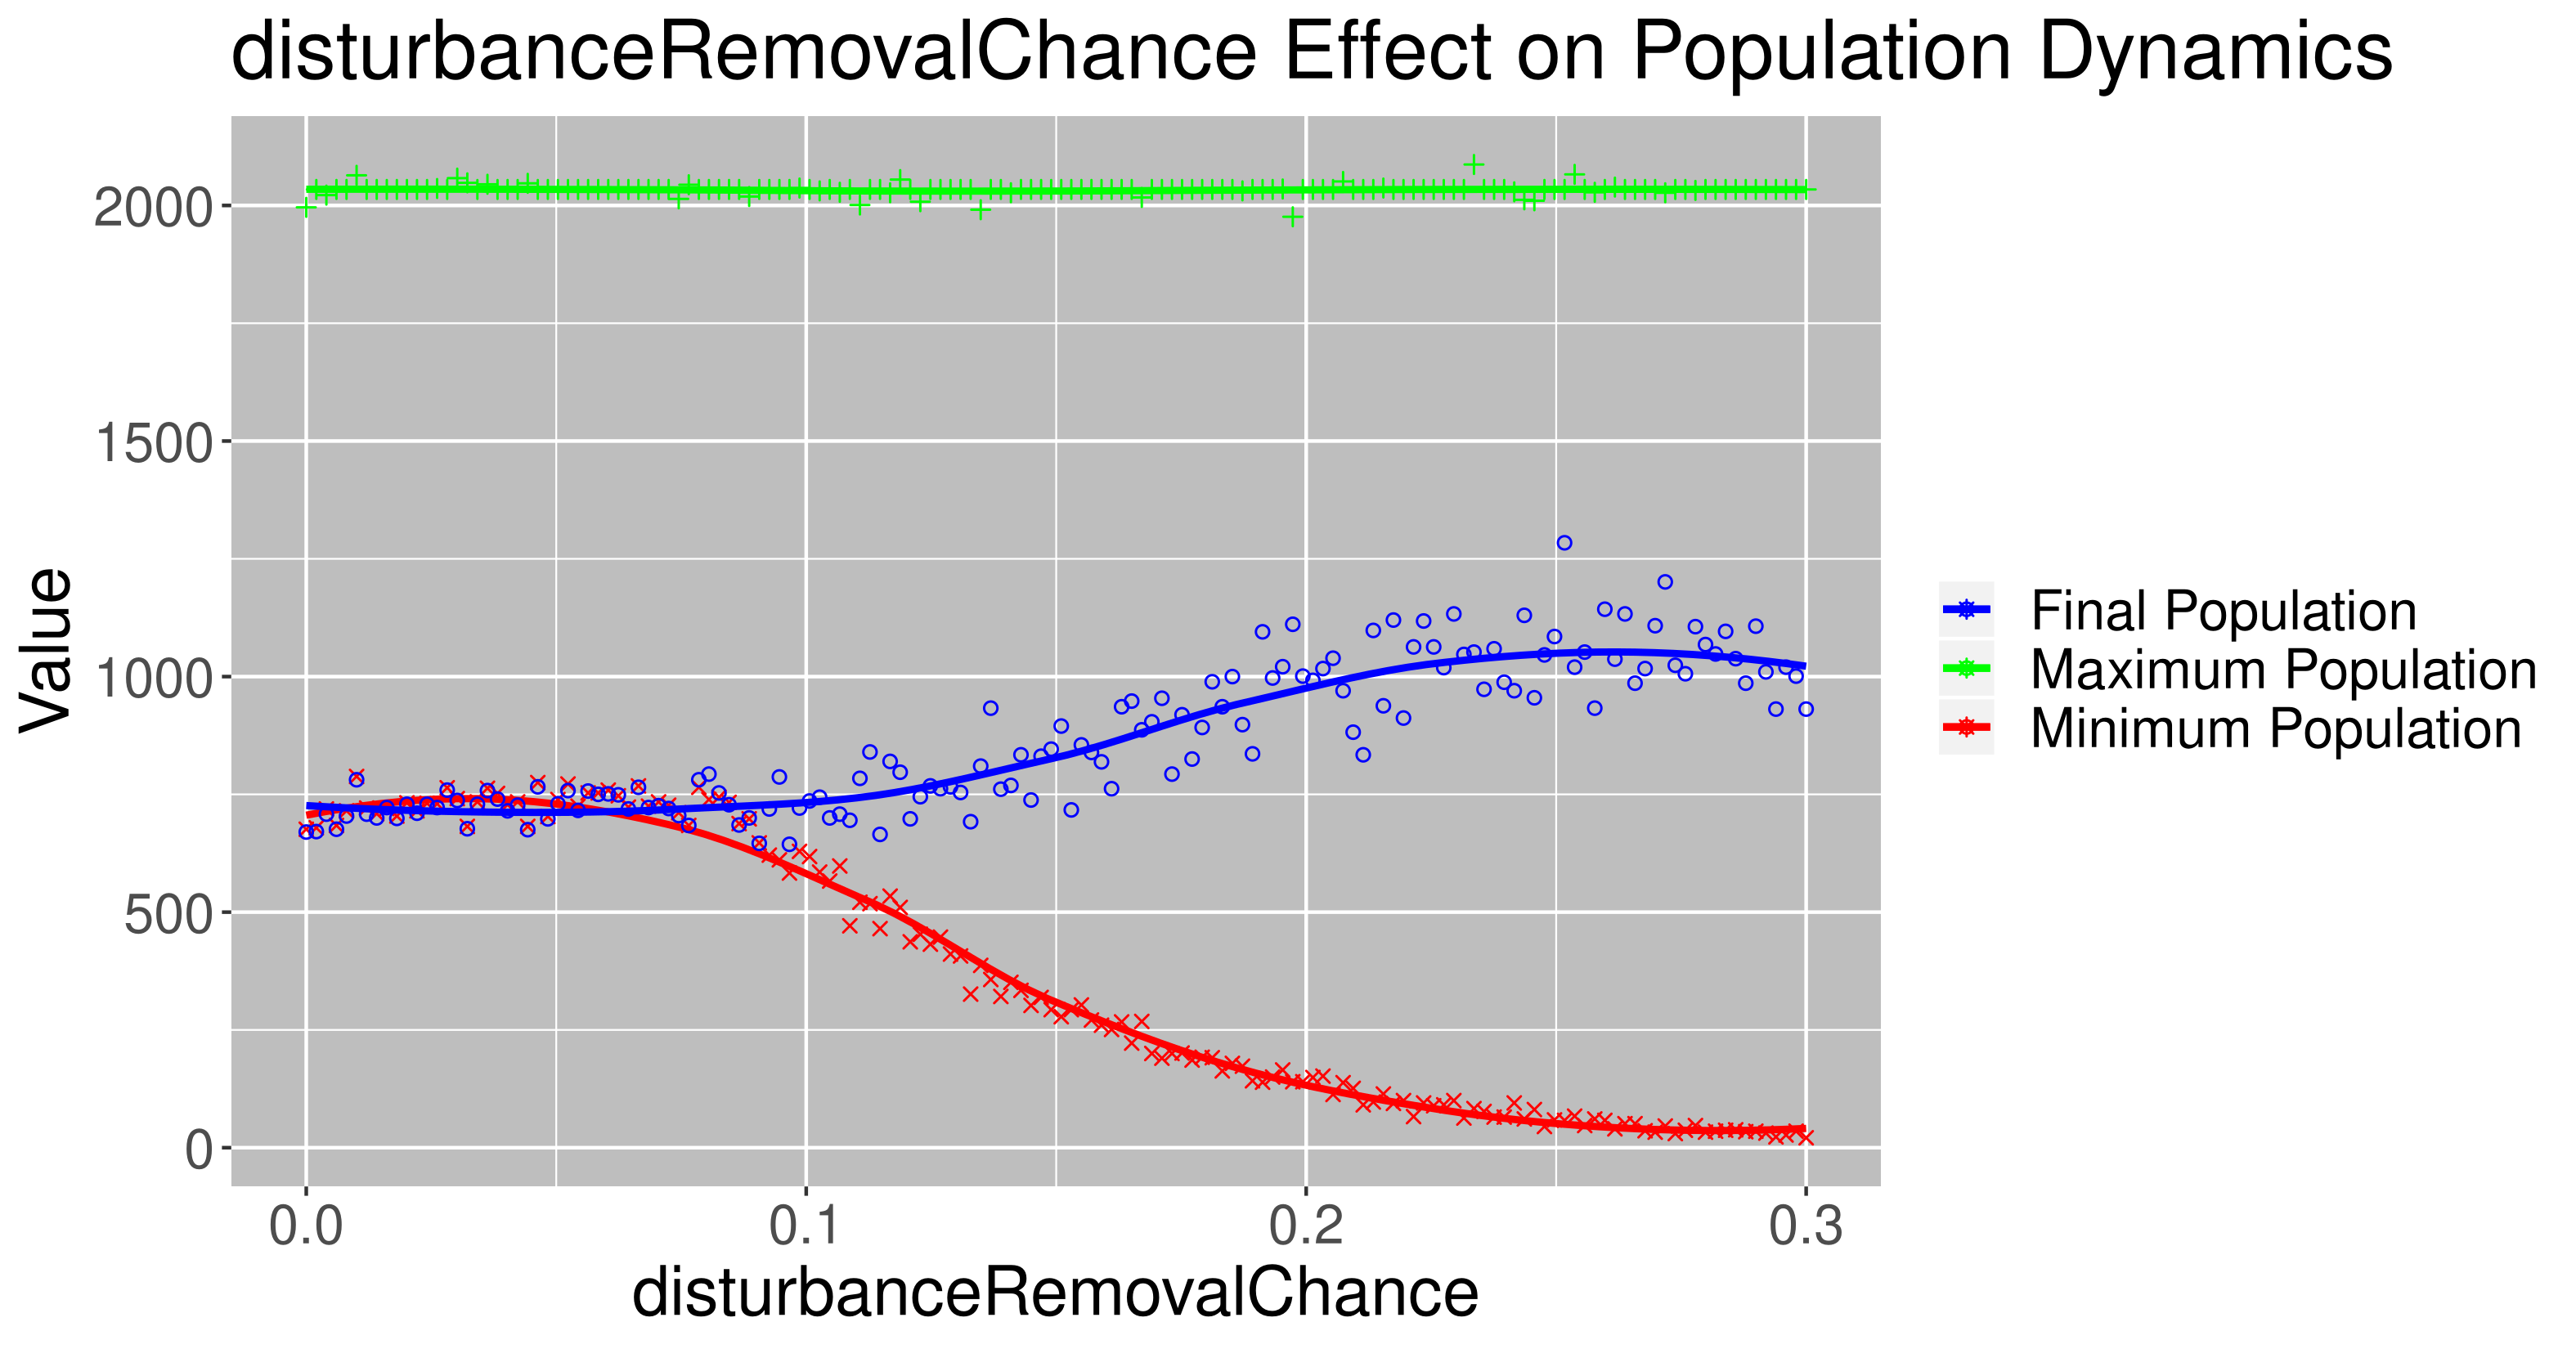
\includegraphics[width=5in]{/home/akara/workspace/R/CHAAHK/REPLACEME/figures/5-1}
	
	Plot corresponding to Figure 5.1 of Kara 2018
	\label{fig:5-1}
\end{figure}

\begin{figure}[H]
	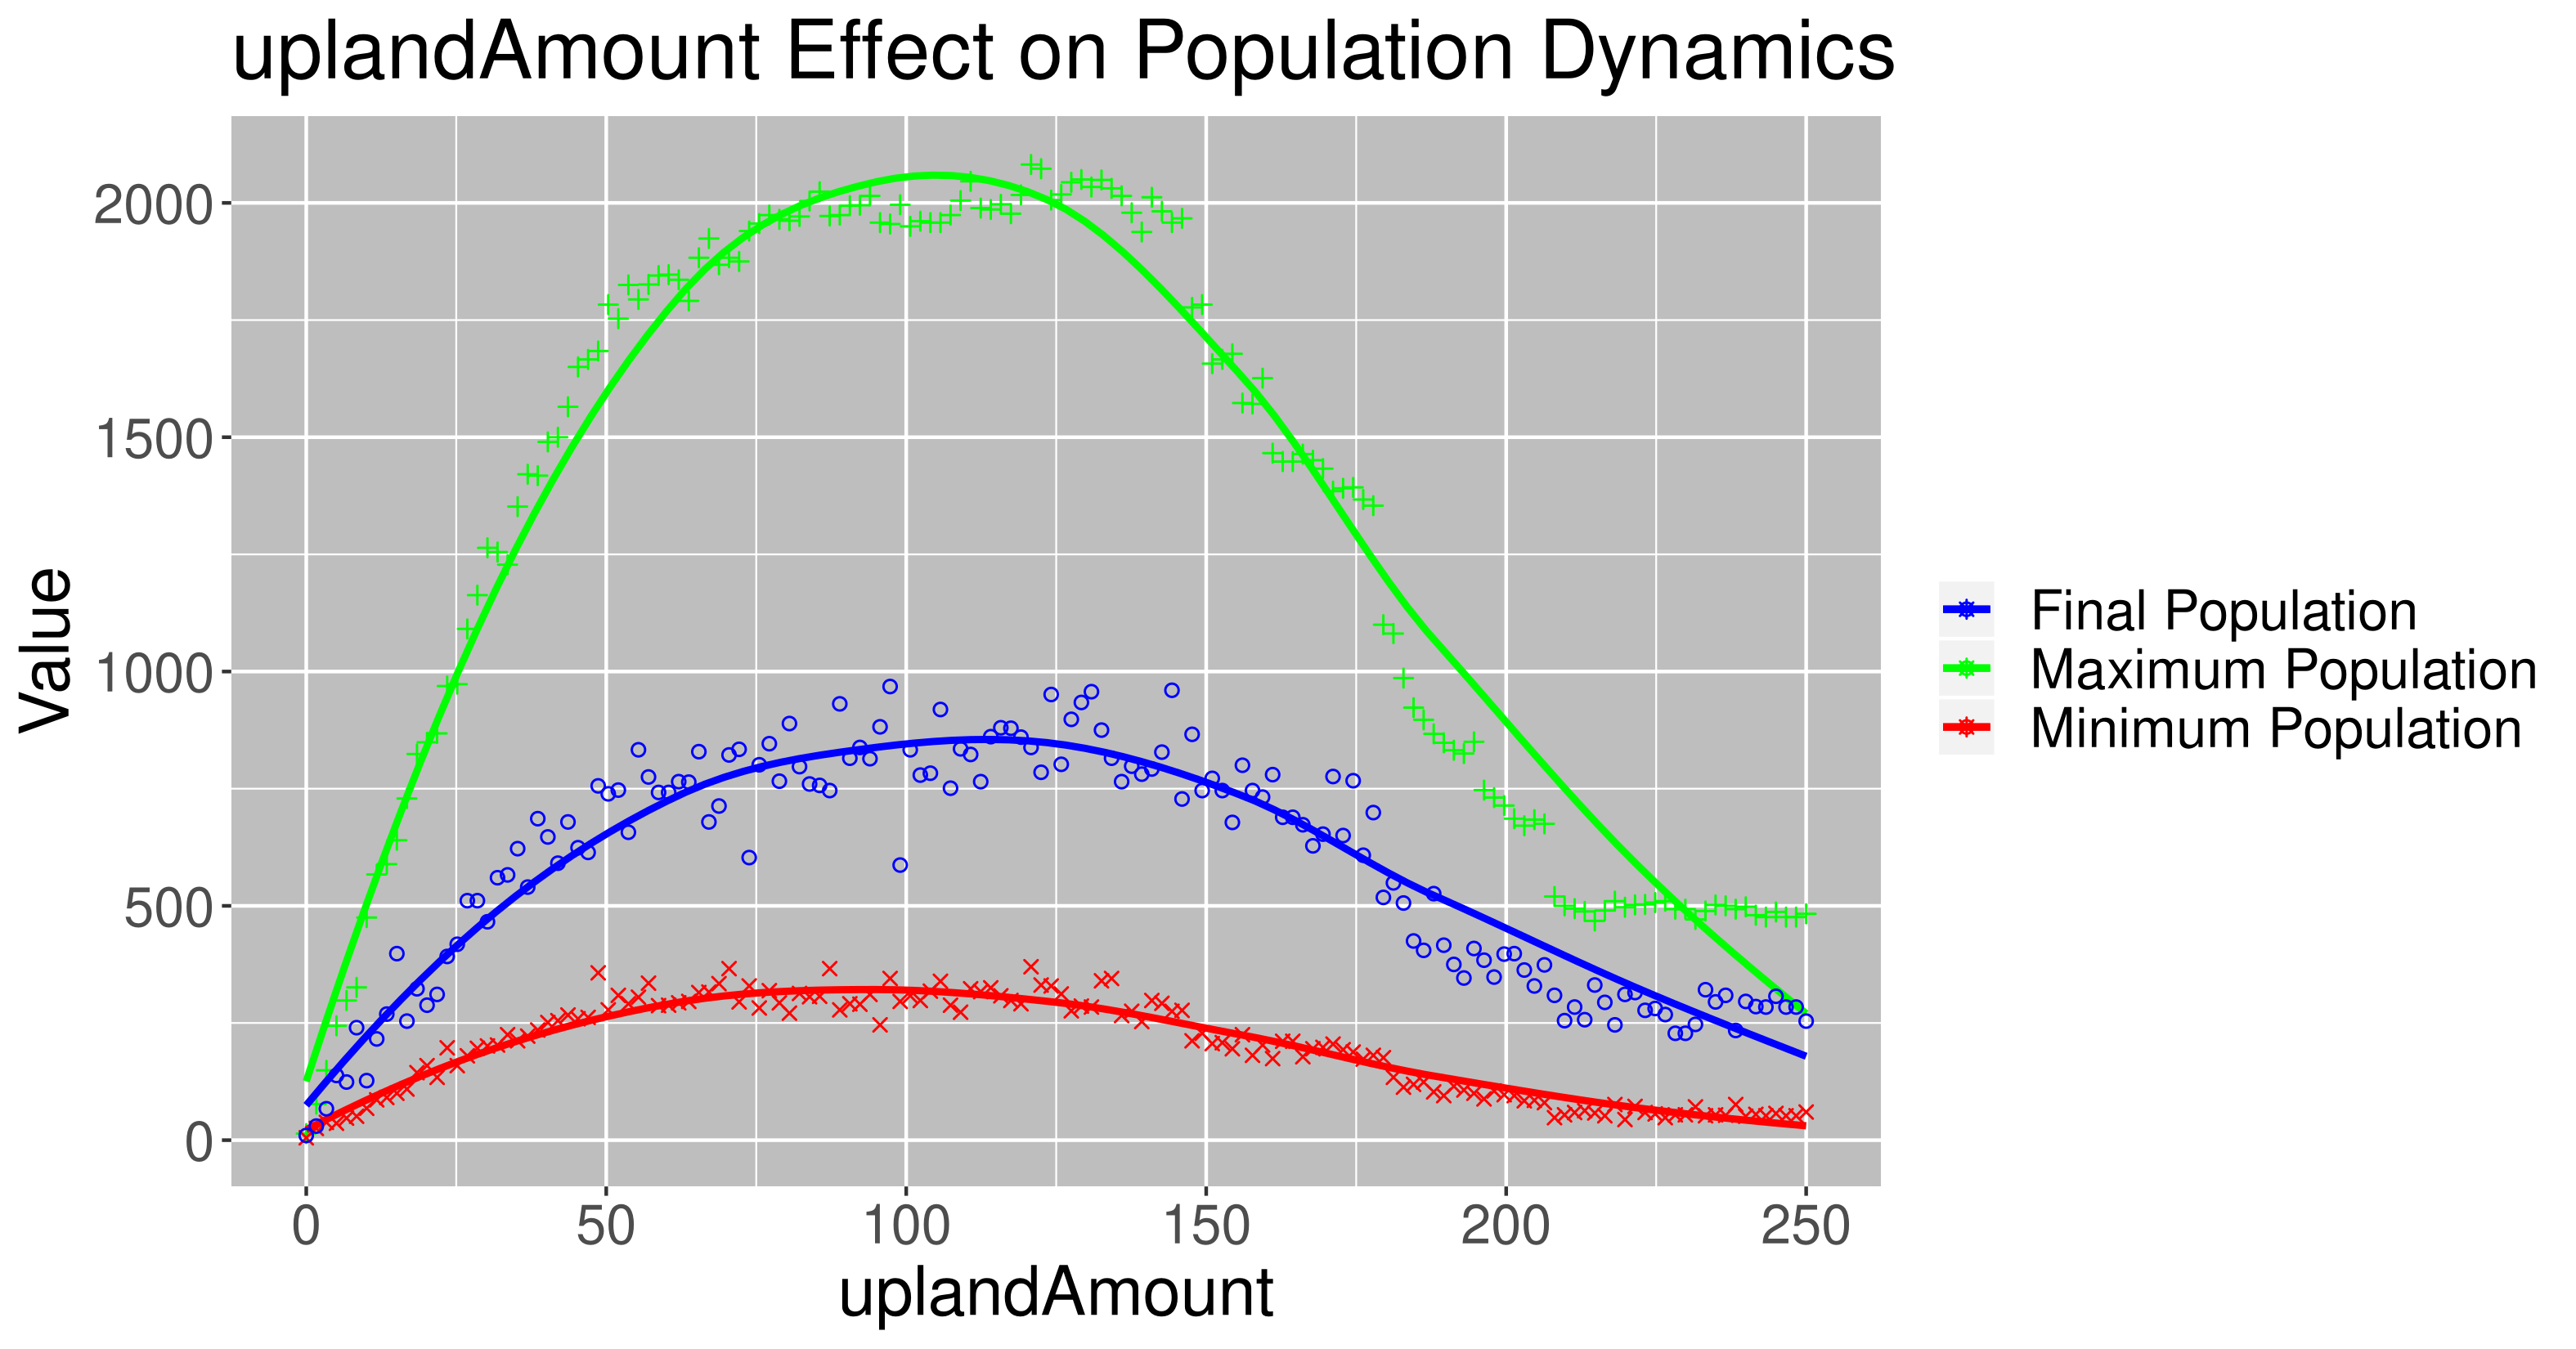
\includegraphics[width=5in]{/home/akara/workspace/R/CHAAHK/REPLACEME/figures/5-2}
	Plot corresponding to Figure 5.2 of Kara 2018
	\label{fig:5-2}
\end{figure}

\begin{figure}[H]
	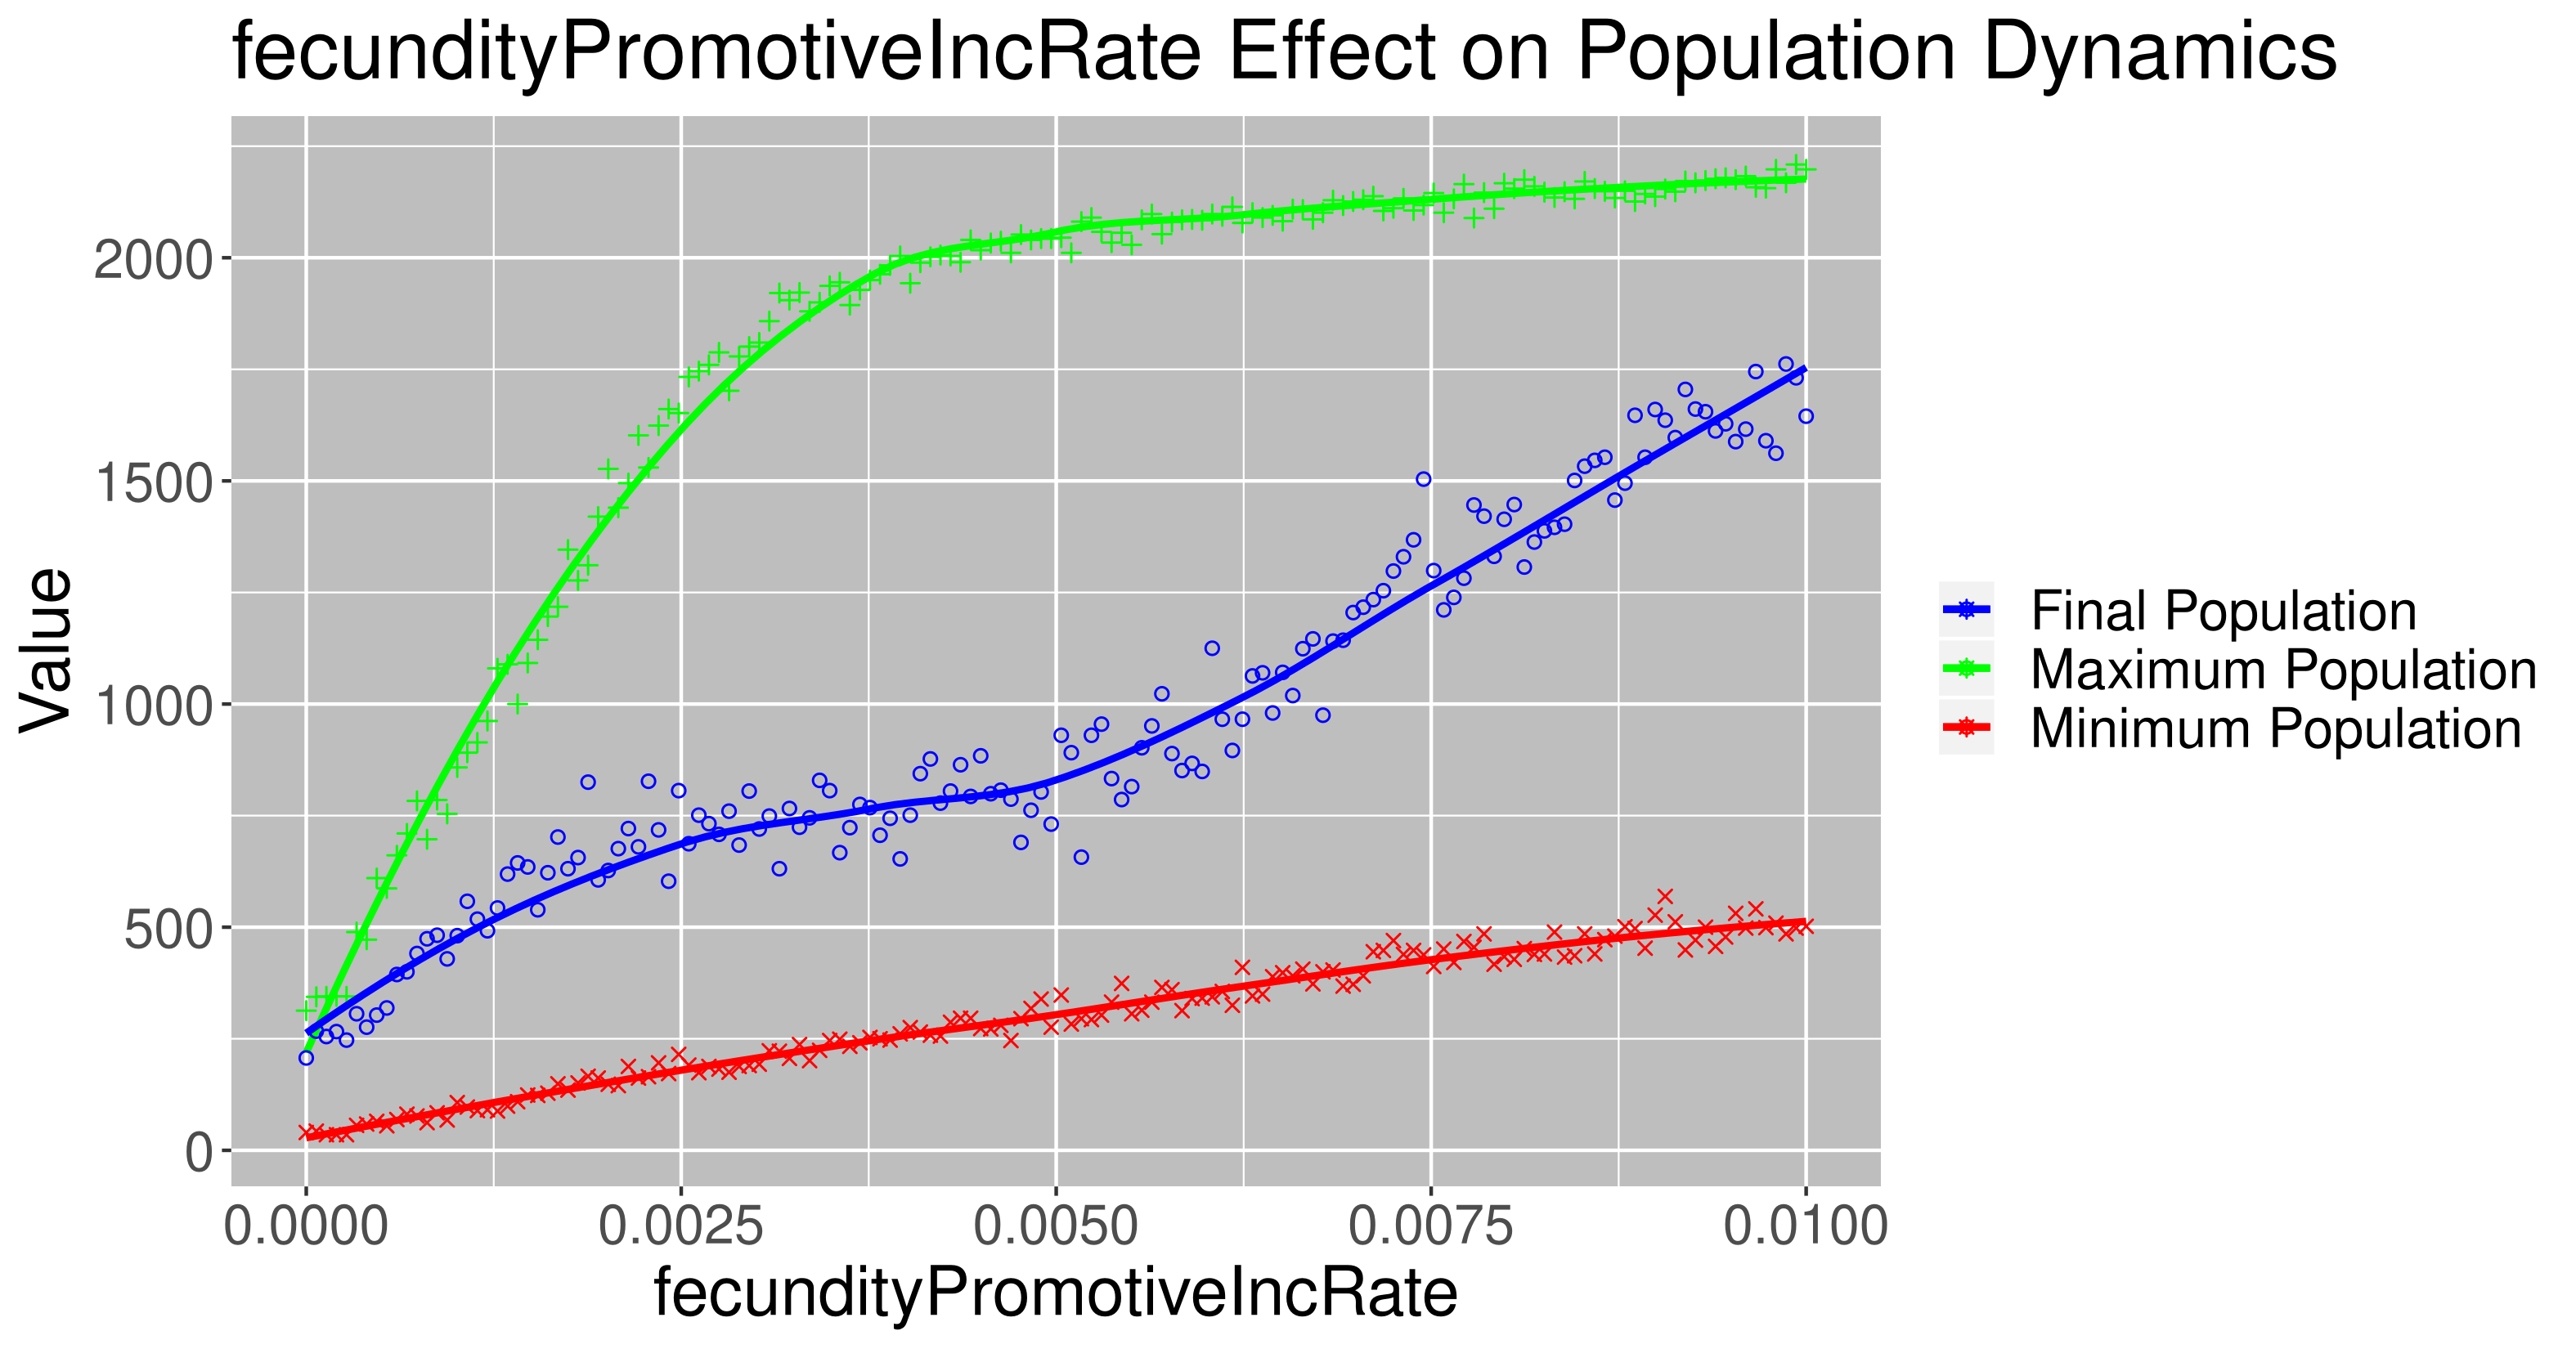
\includegraphics[width=5in]{/home/akara/workspace/R/CHAAHK/REPLACEME/figures/5-3}
	Plot corresponding to Figure 5.3 of Kara 2018
	\label{fig:5-3}
\end{figure}
\begin{figure}[H]
	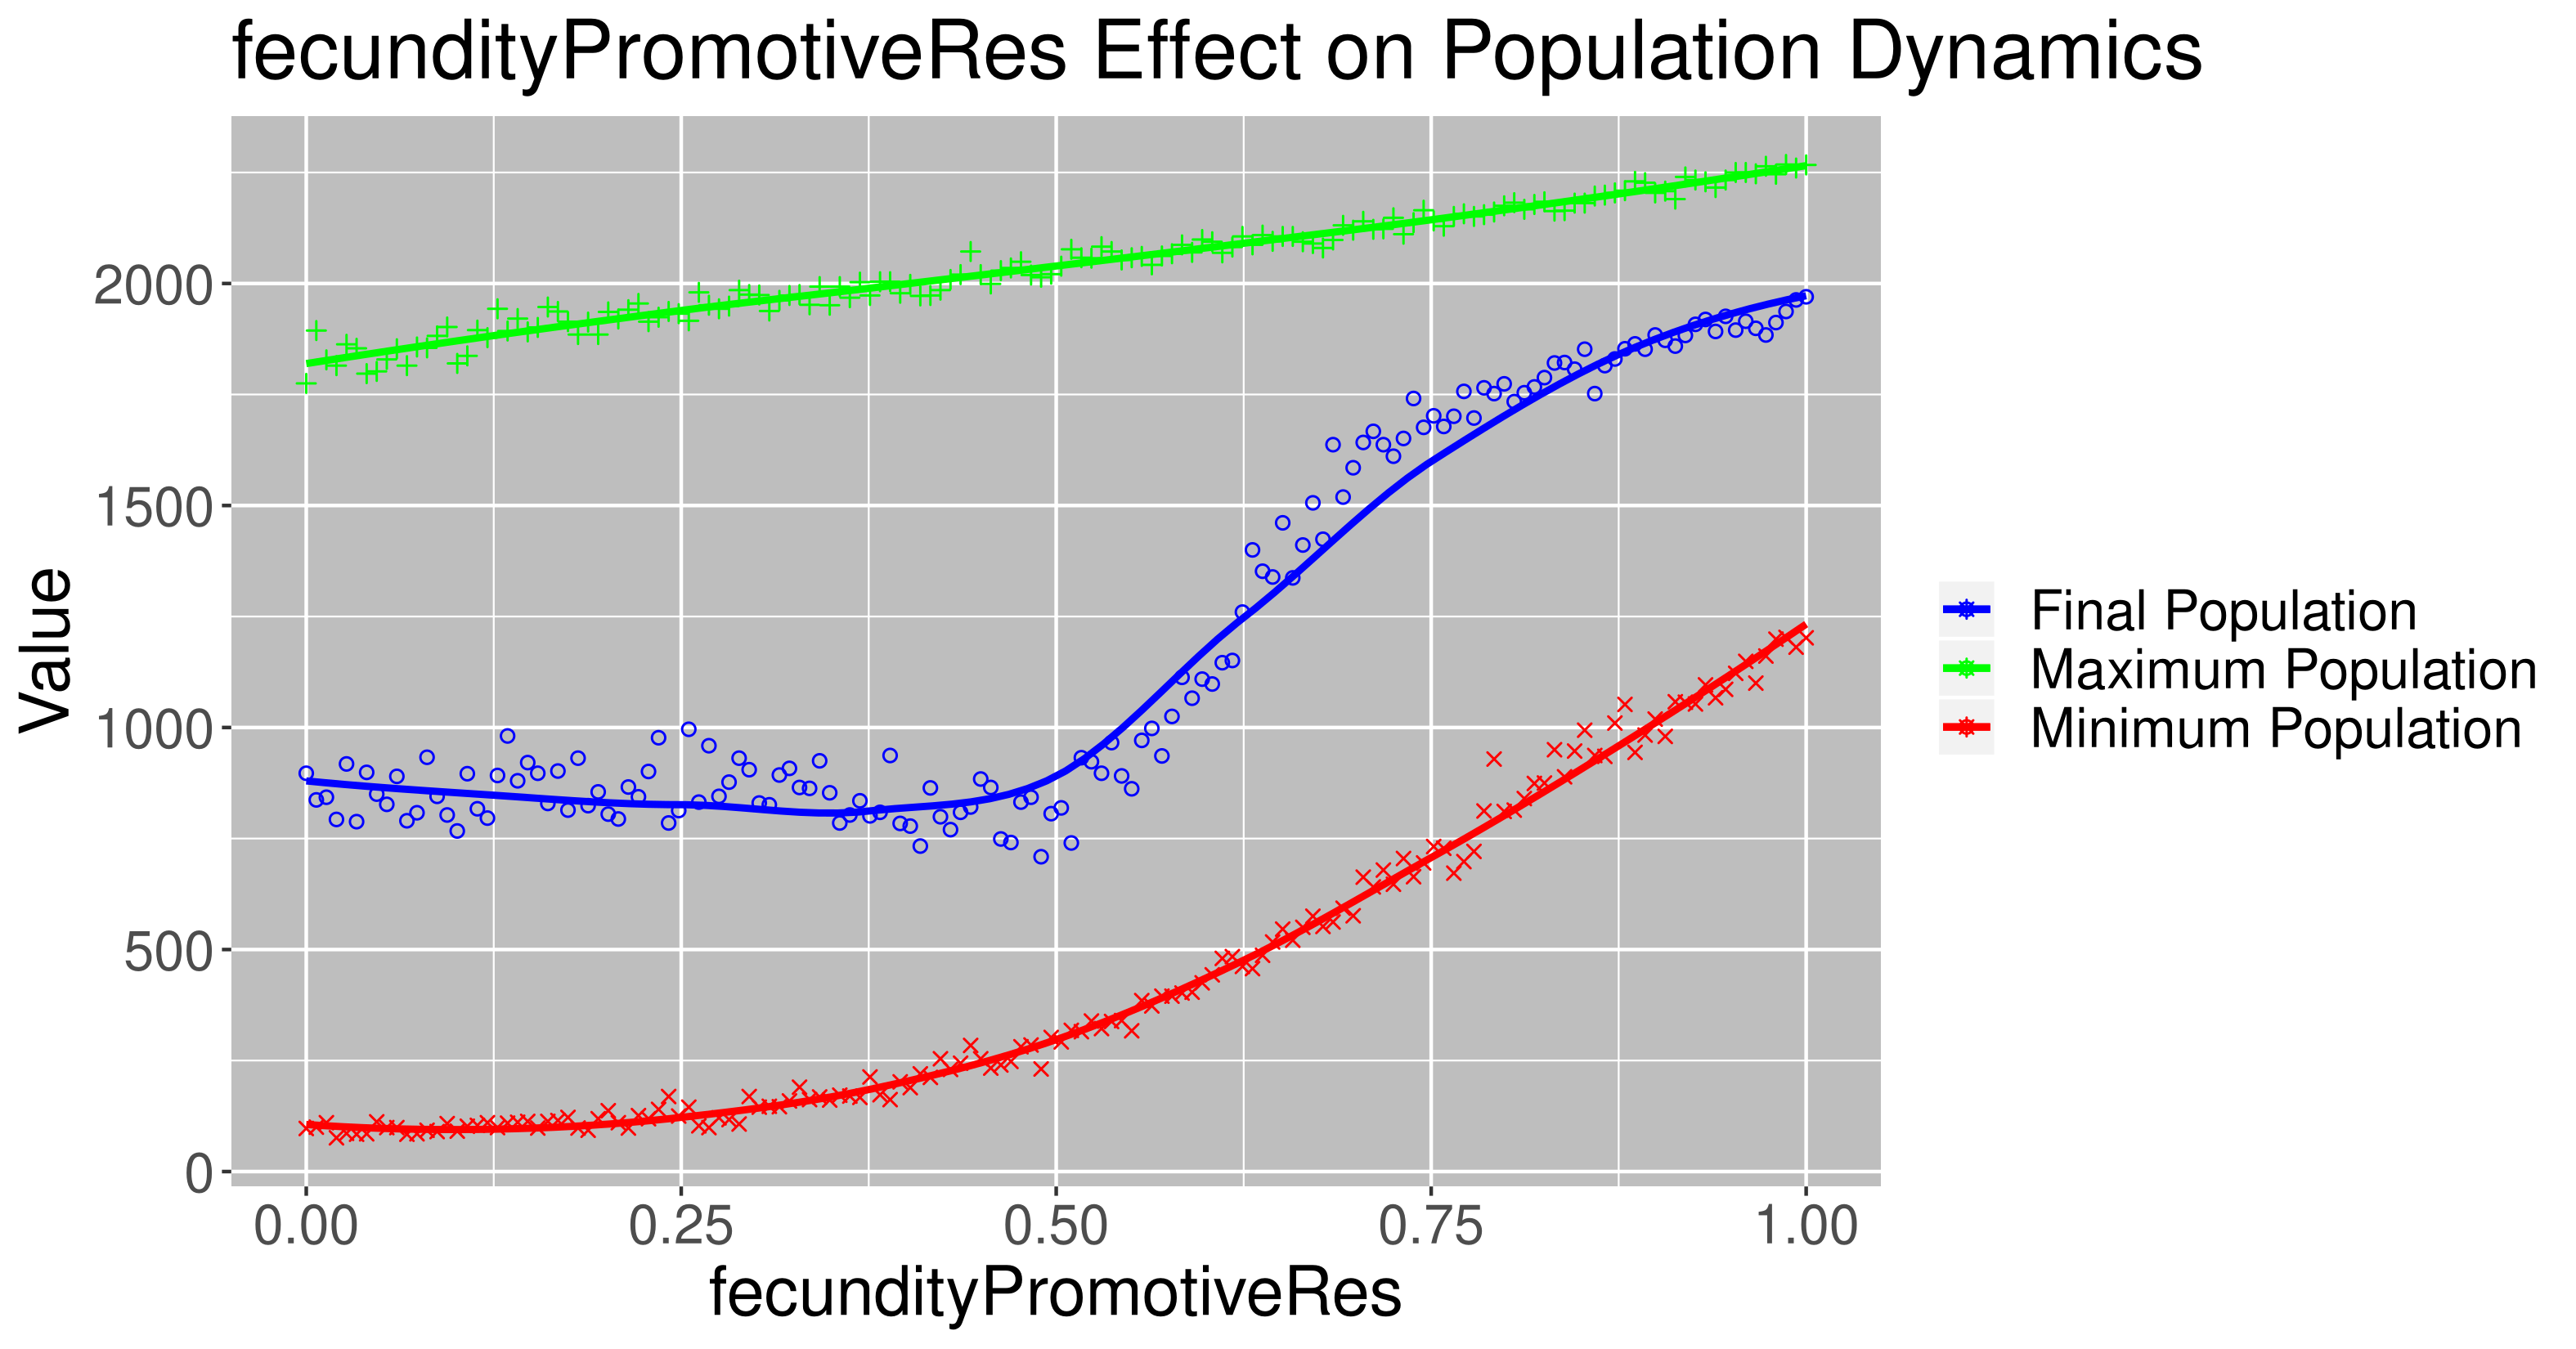
\includegraphics[width=5in]{/home/akara/workspace/R/CHAAHK/REPLACEME/figures/5-4}
	Plot corresponding to Figure 5.4 of Kara 2018
	\label{fig:5-4}
\end{figure}
\begin{figure}[H]
	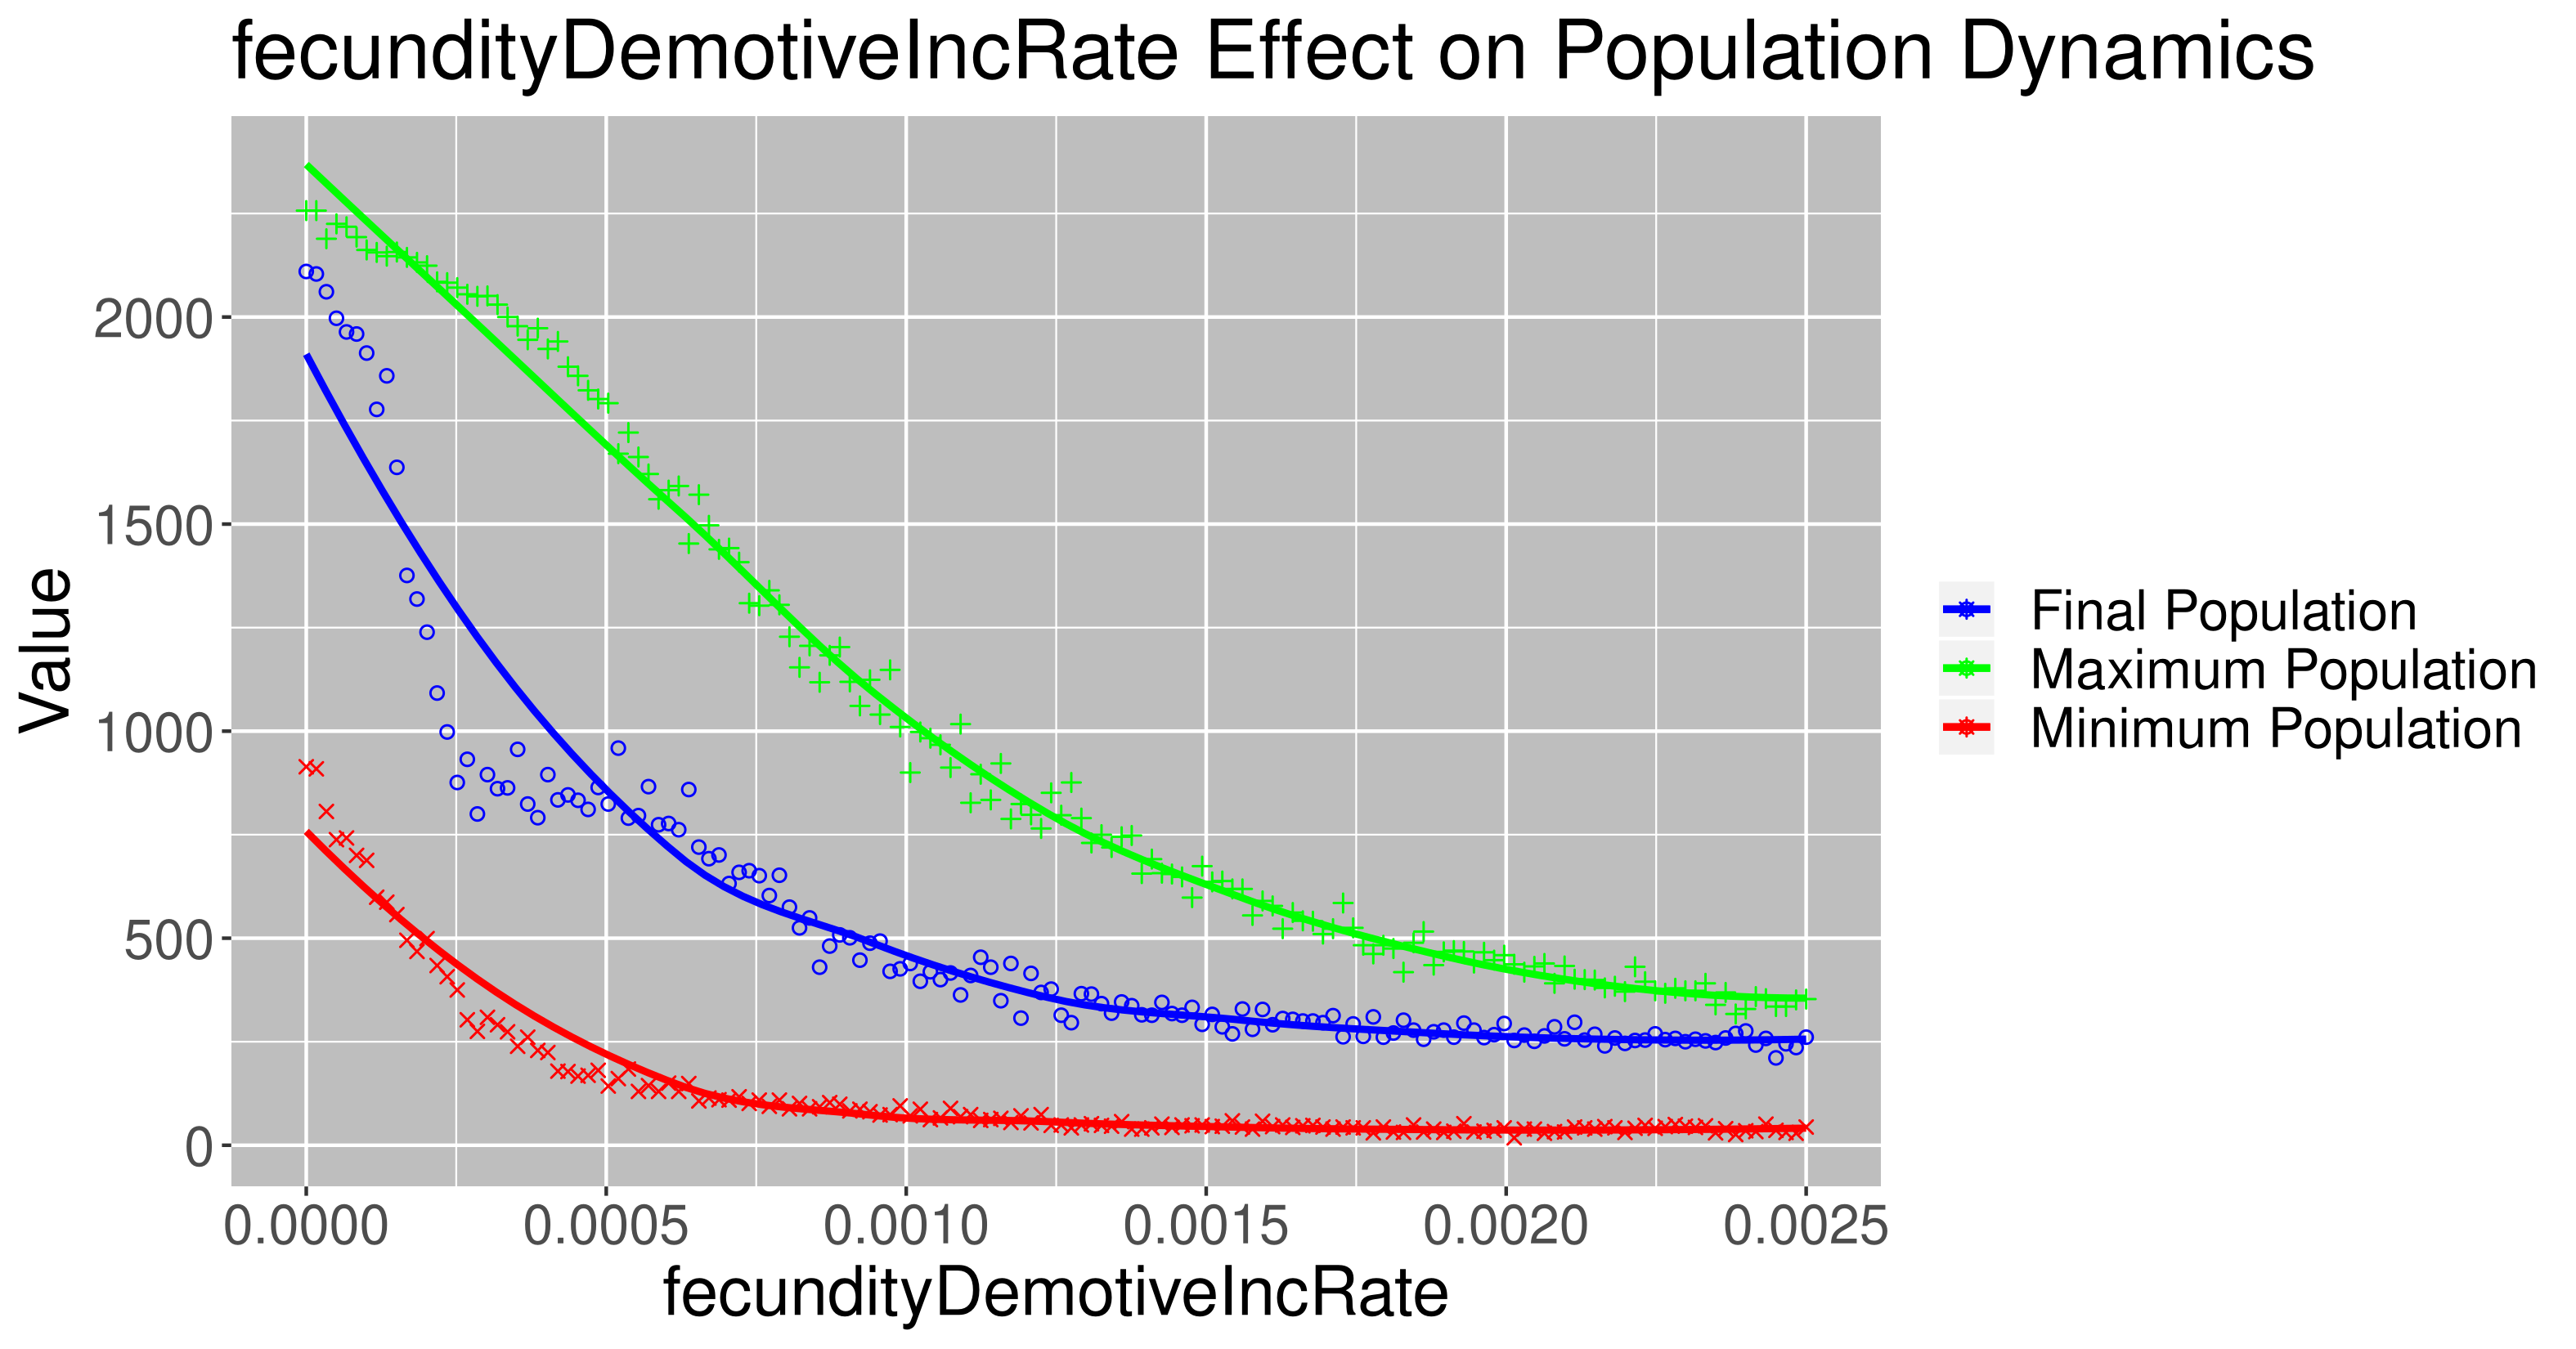
\includegraphics[width=5in]{/home/akara/workspace/R/CHAAHK/REPLACEME/figures/5-5}
	Plot corresponding to Figure 5.5 of Kara 2018
	\label{fig:5-5}
\end{figure}
\begin{figure}[H]
	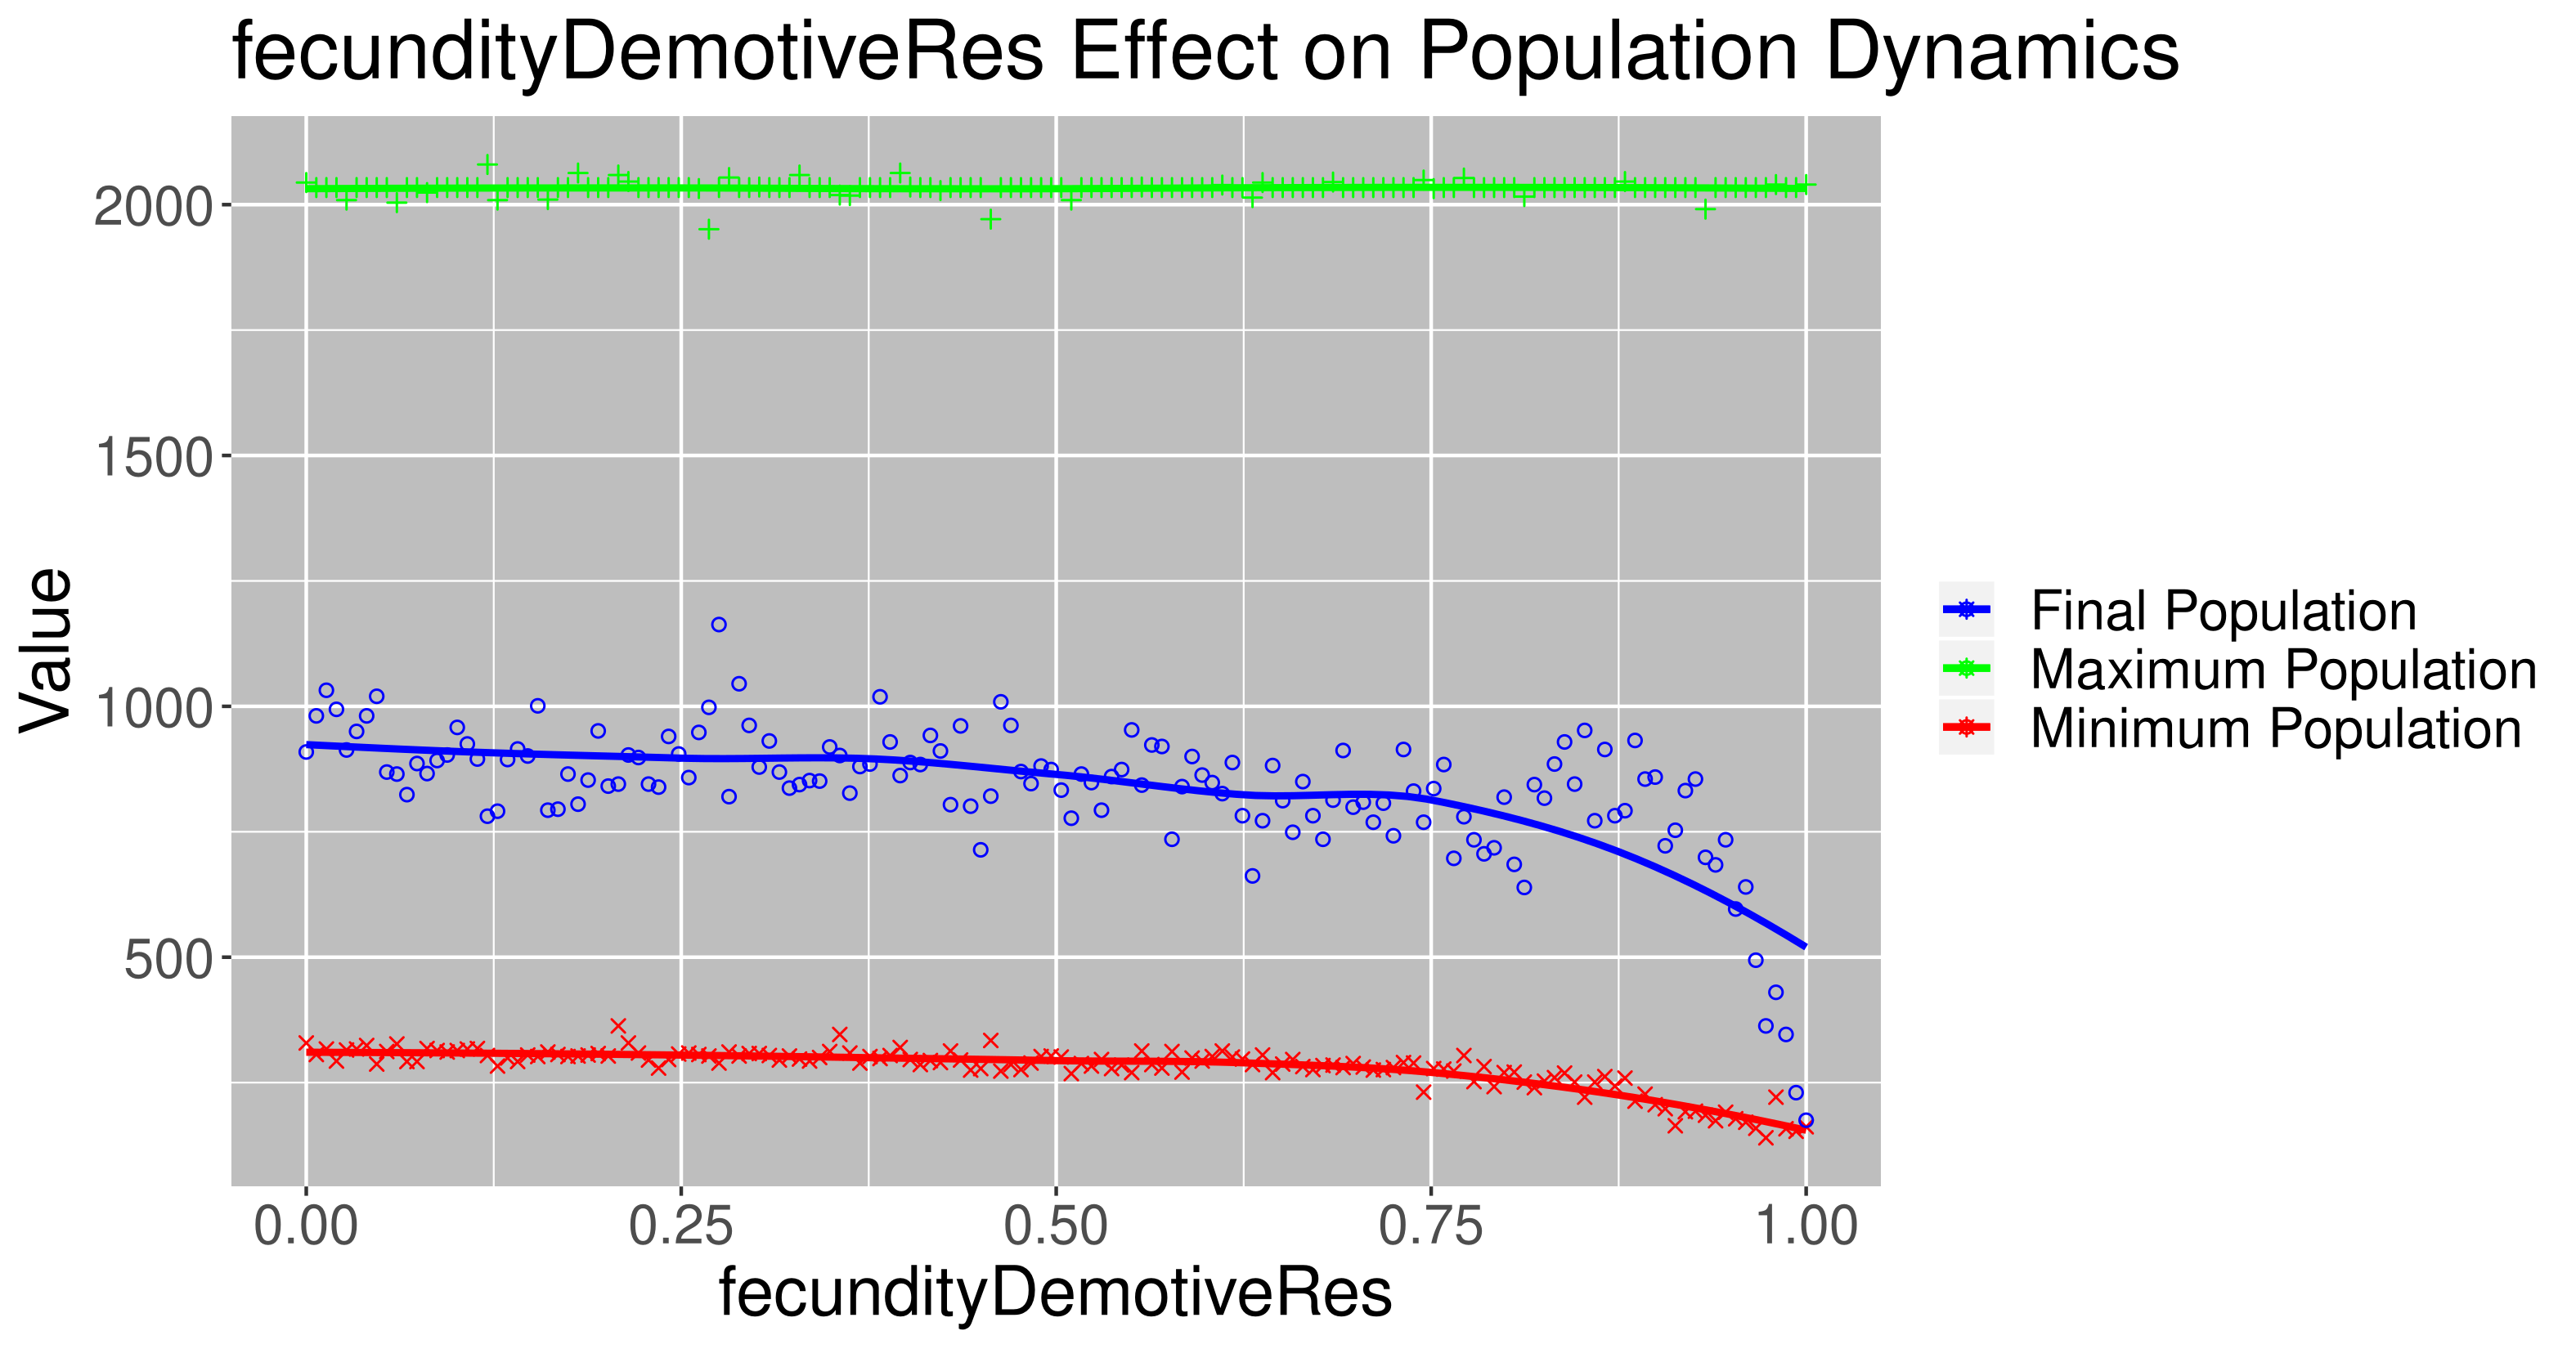
\includegraphics[width=5in]{/home/akara/workspace/R/CHAAHK/REPLACEME/figures/5-6}
	Plot corresponding to Figure 5.6 of Kara 2018
	\label{fig:5-6}
\end{figure}
\begin{figure}[H]
	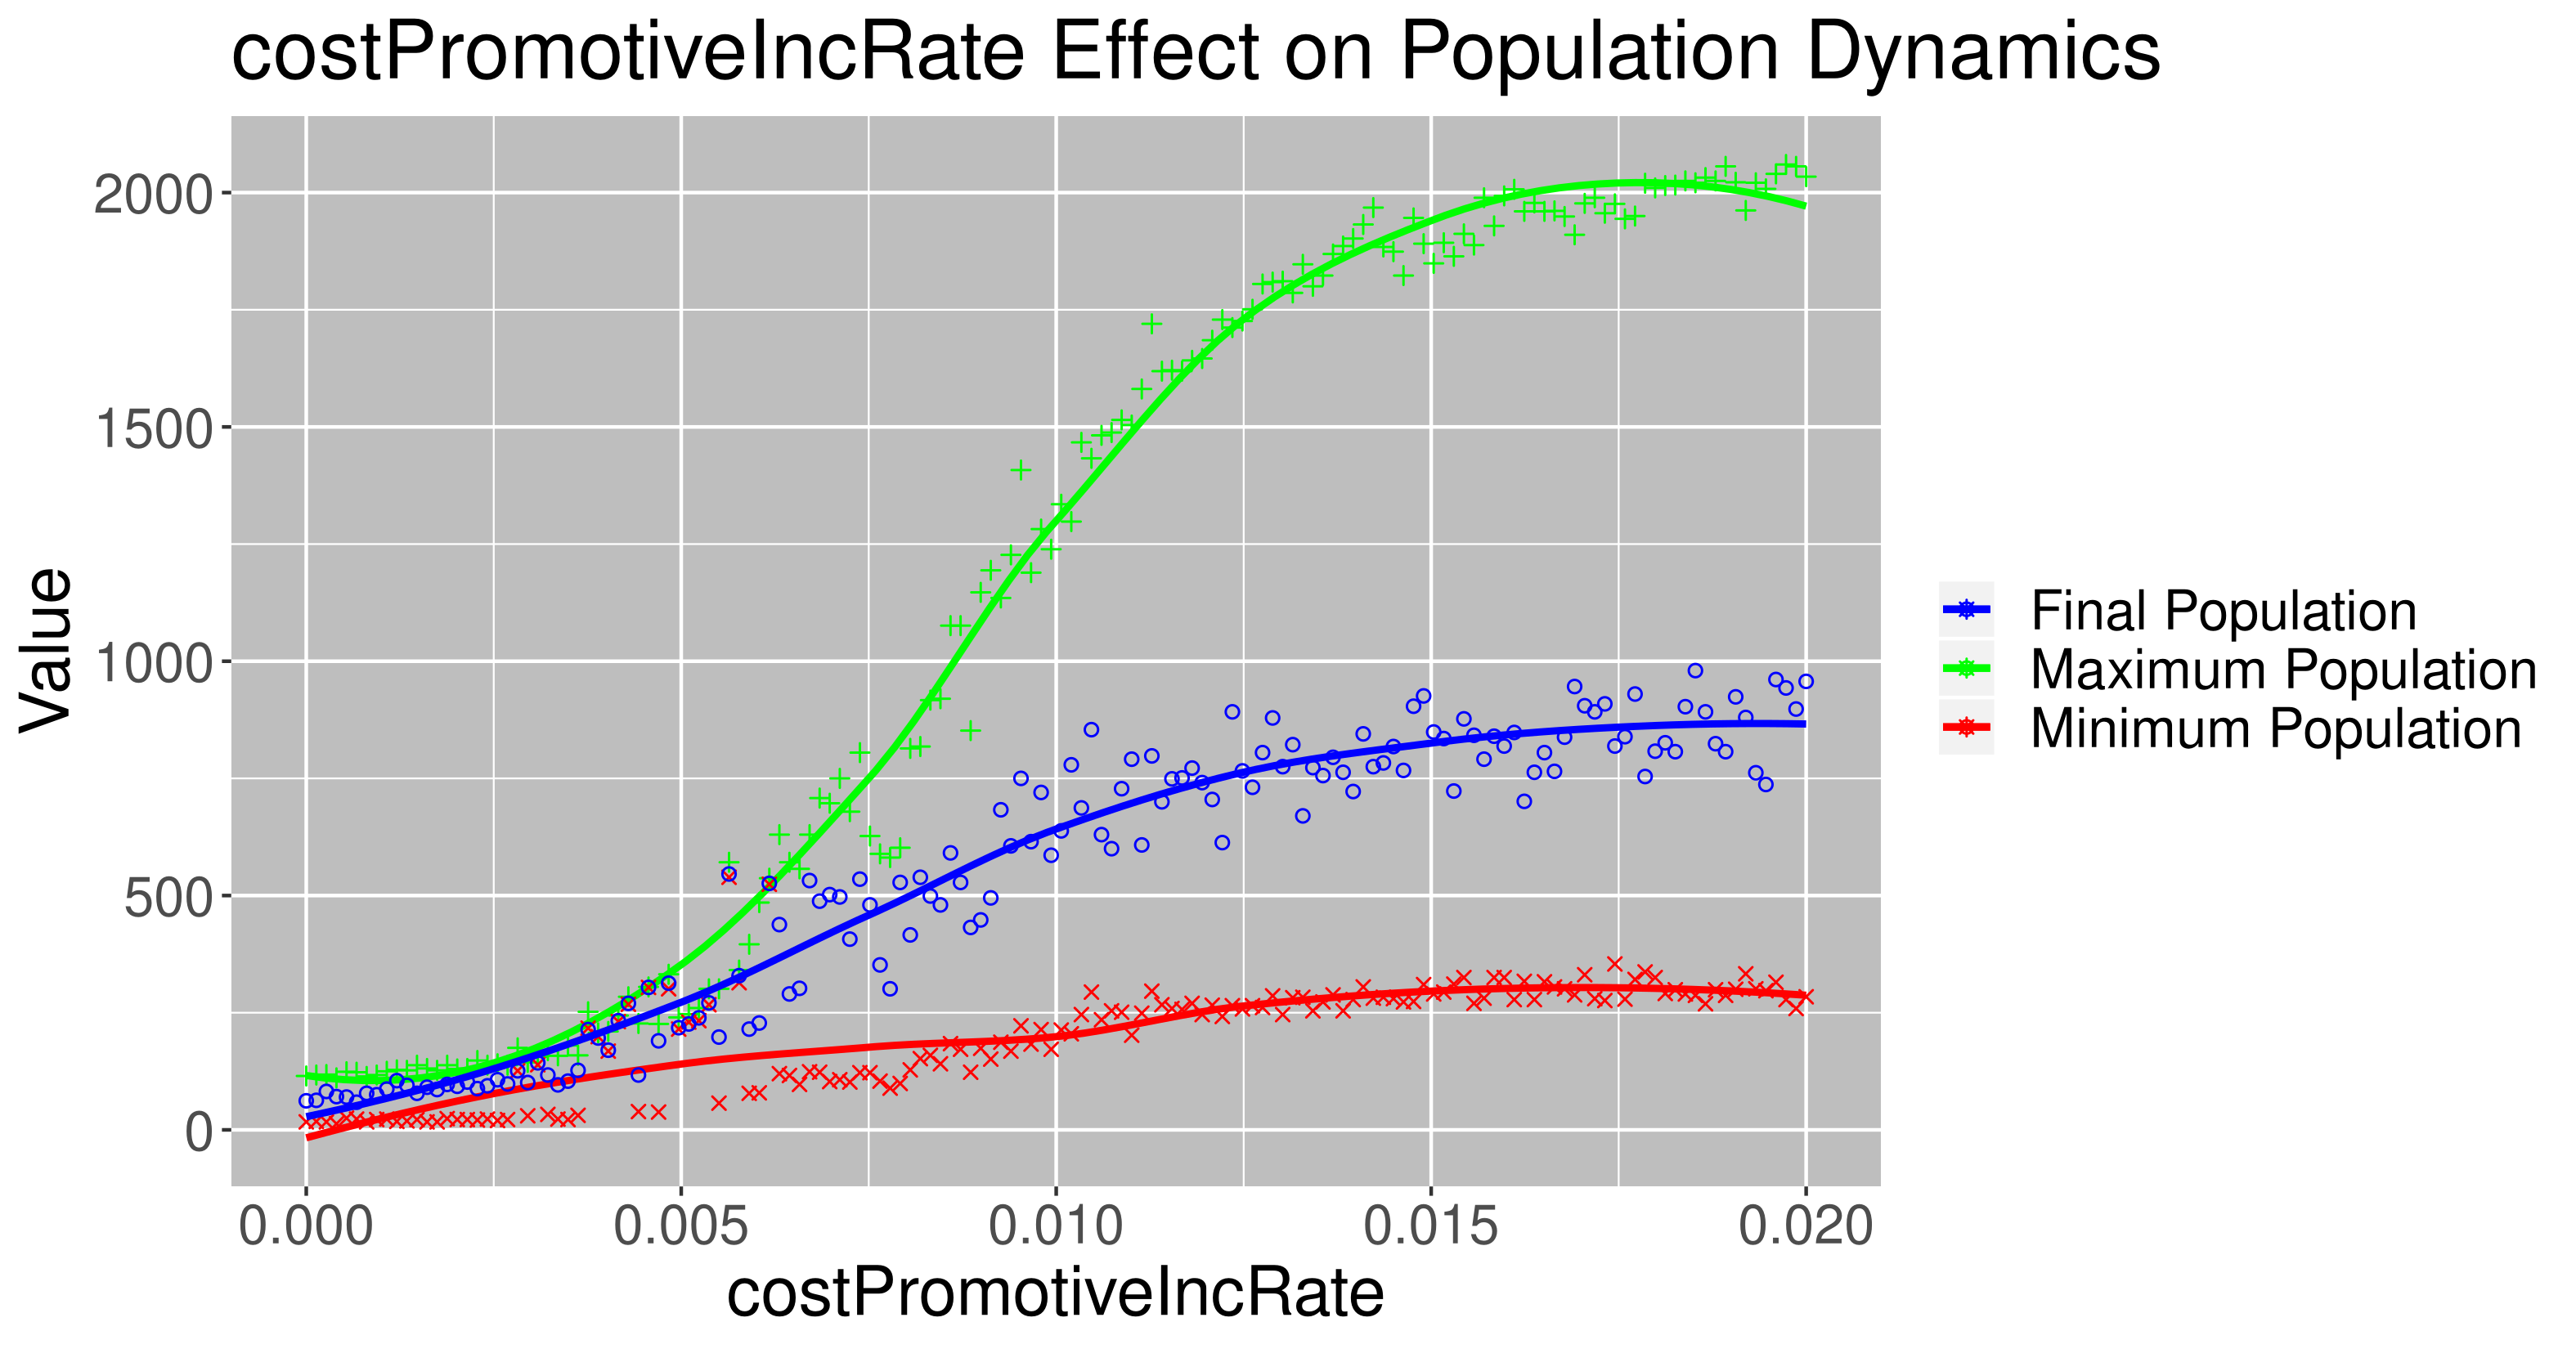
\includegraphics[width=5in]{/home/akara/workspace/R/CHAAHK/REPLACEME/figures/5-7}
	Plot corresponding to Figure 5.7 of Kara 2018
	\label{fig:5-7}
\end{figure}
\begin{figure}[H]
	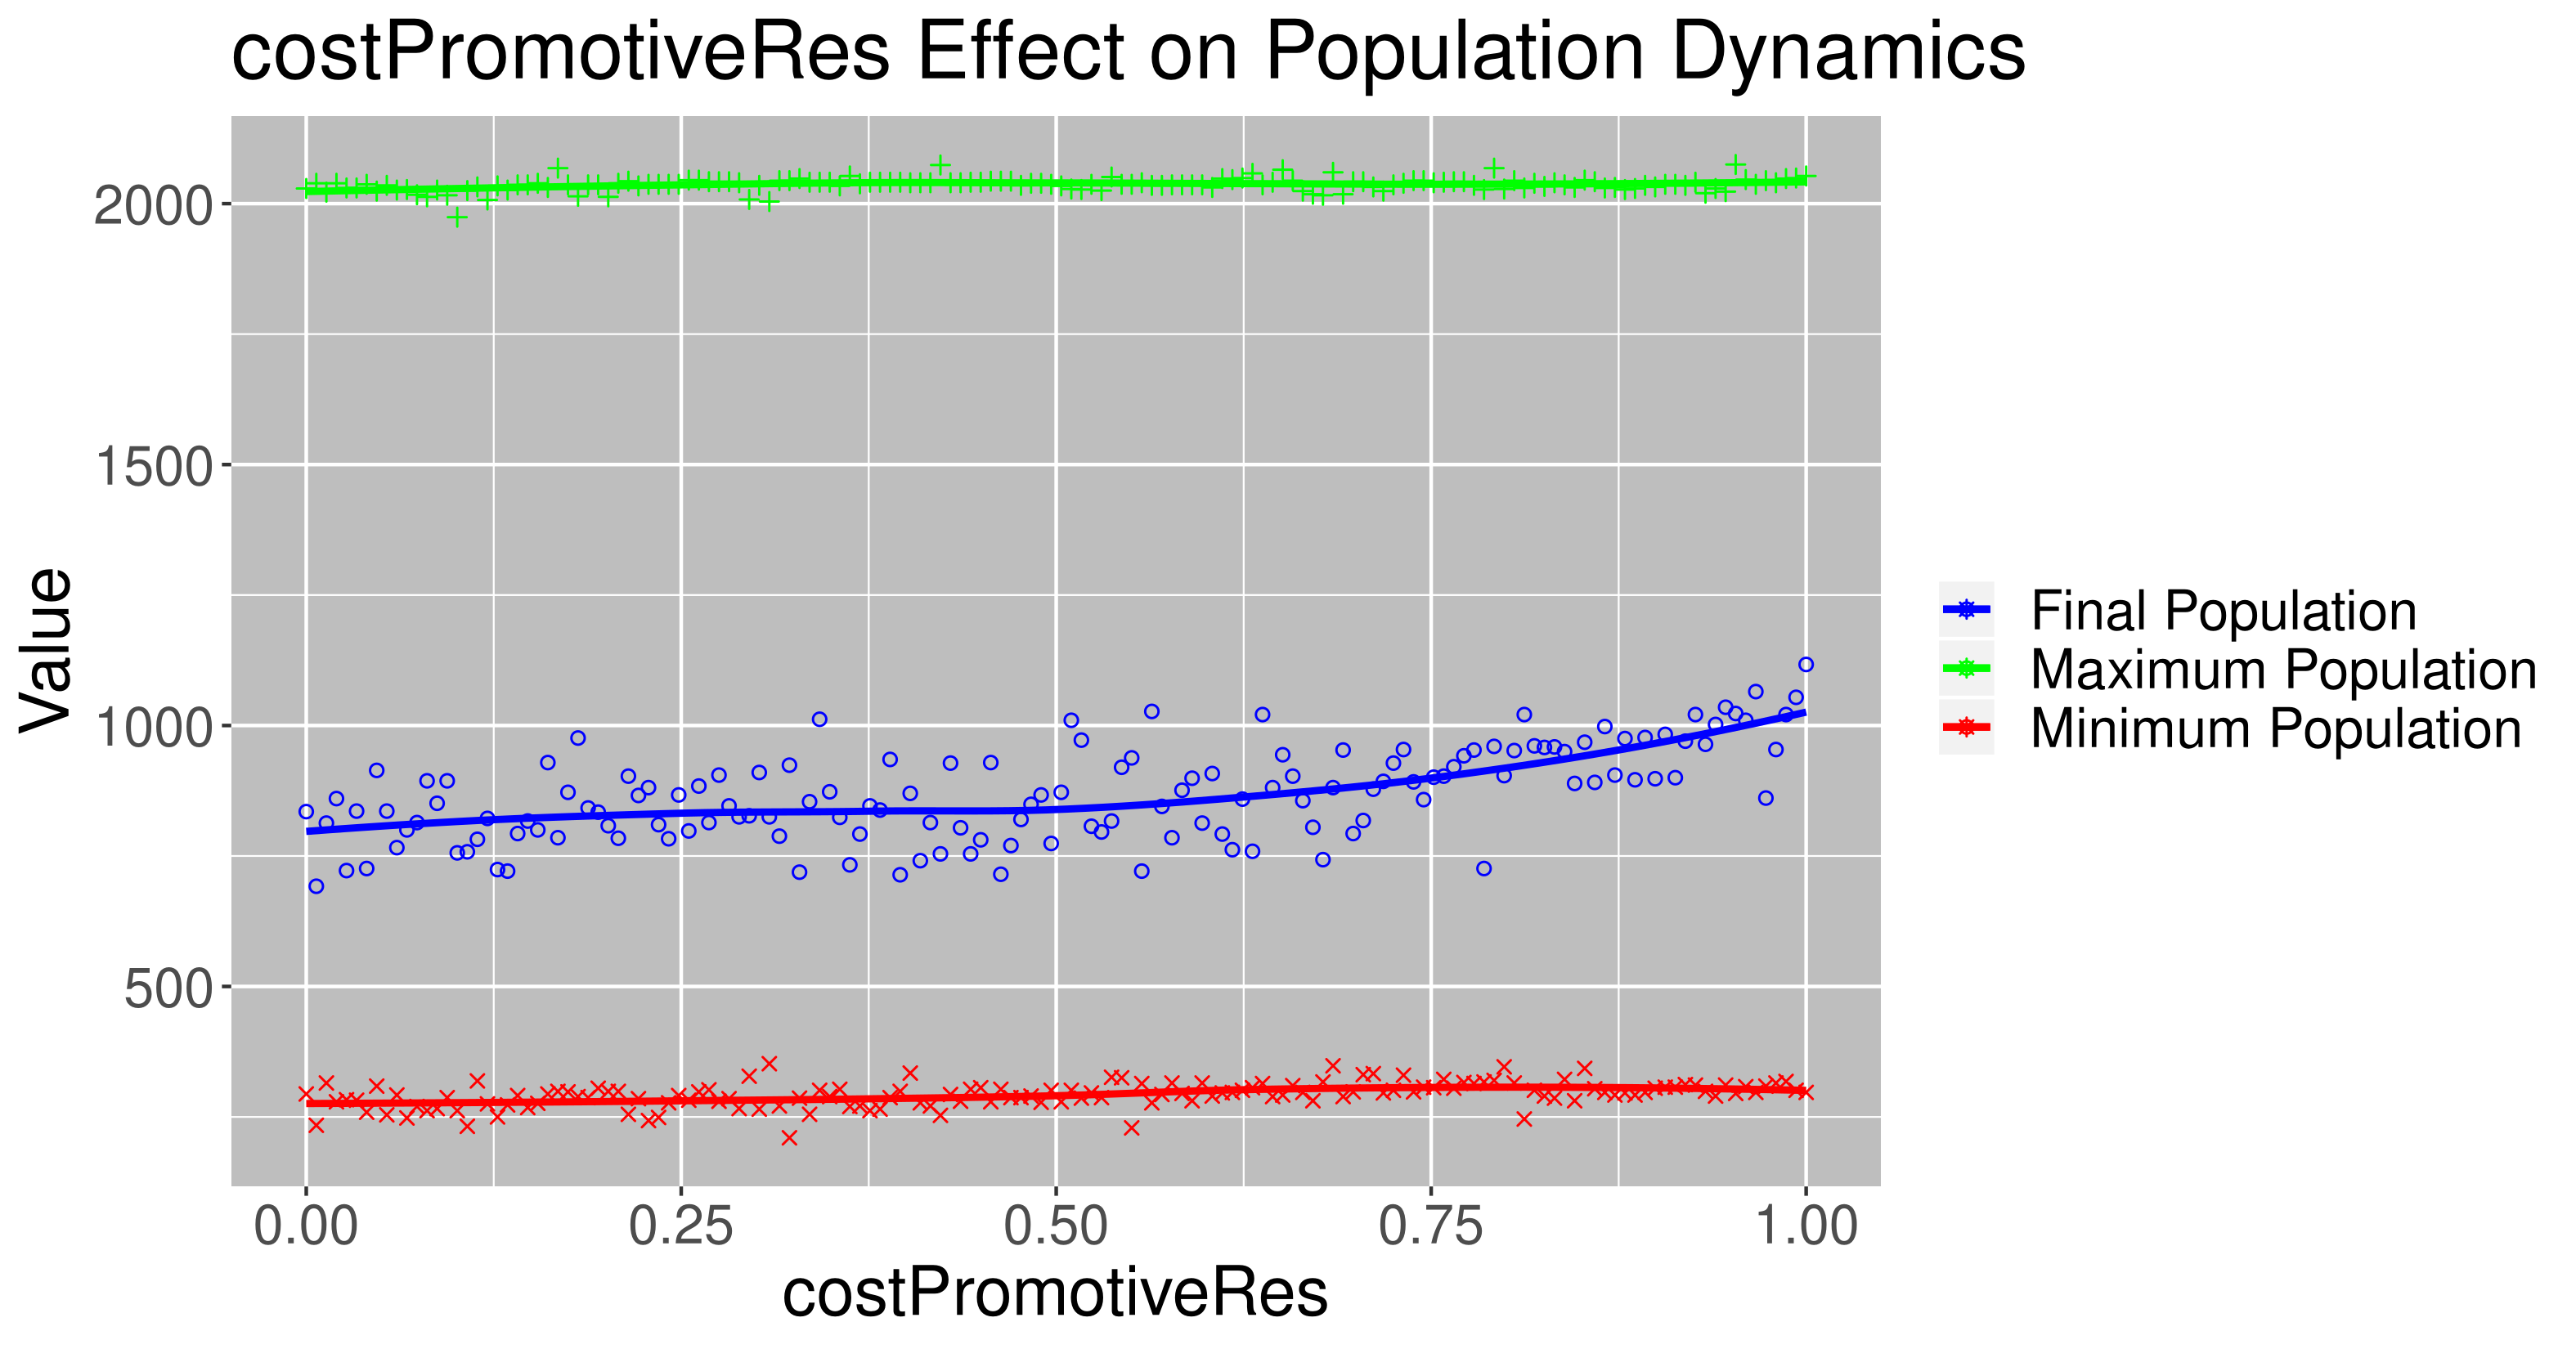
\includegraphics[width=5in]{/home/akara/workspace/R/CHAAHK/REPLACEME/figures/5-8}
	Plot corresponding to Figure 5.8 of Kara 2018
	\label{fig:5-8}
\end{figure}
\begin{figure}[H]
	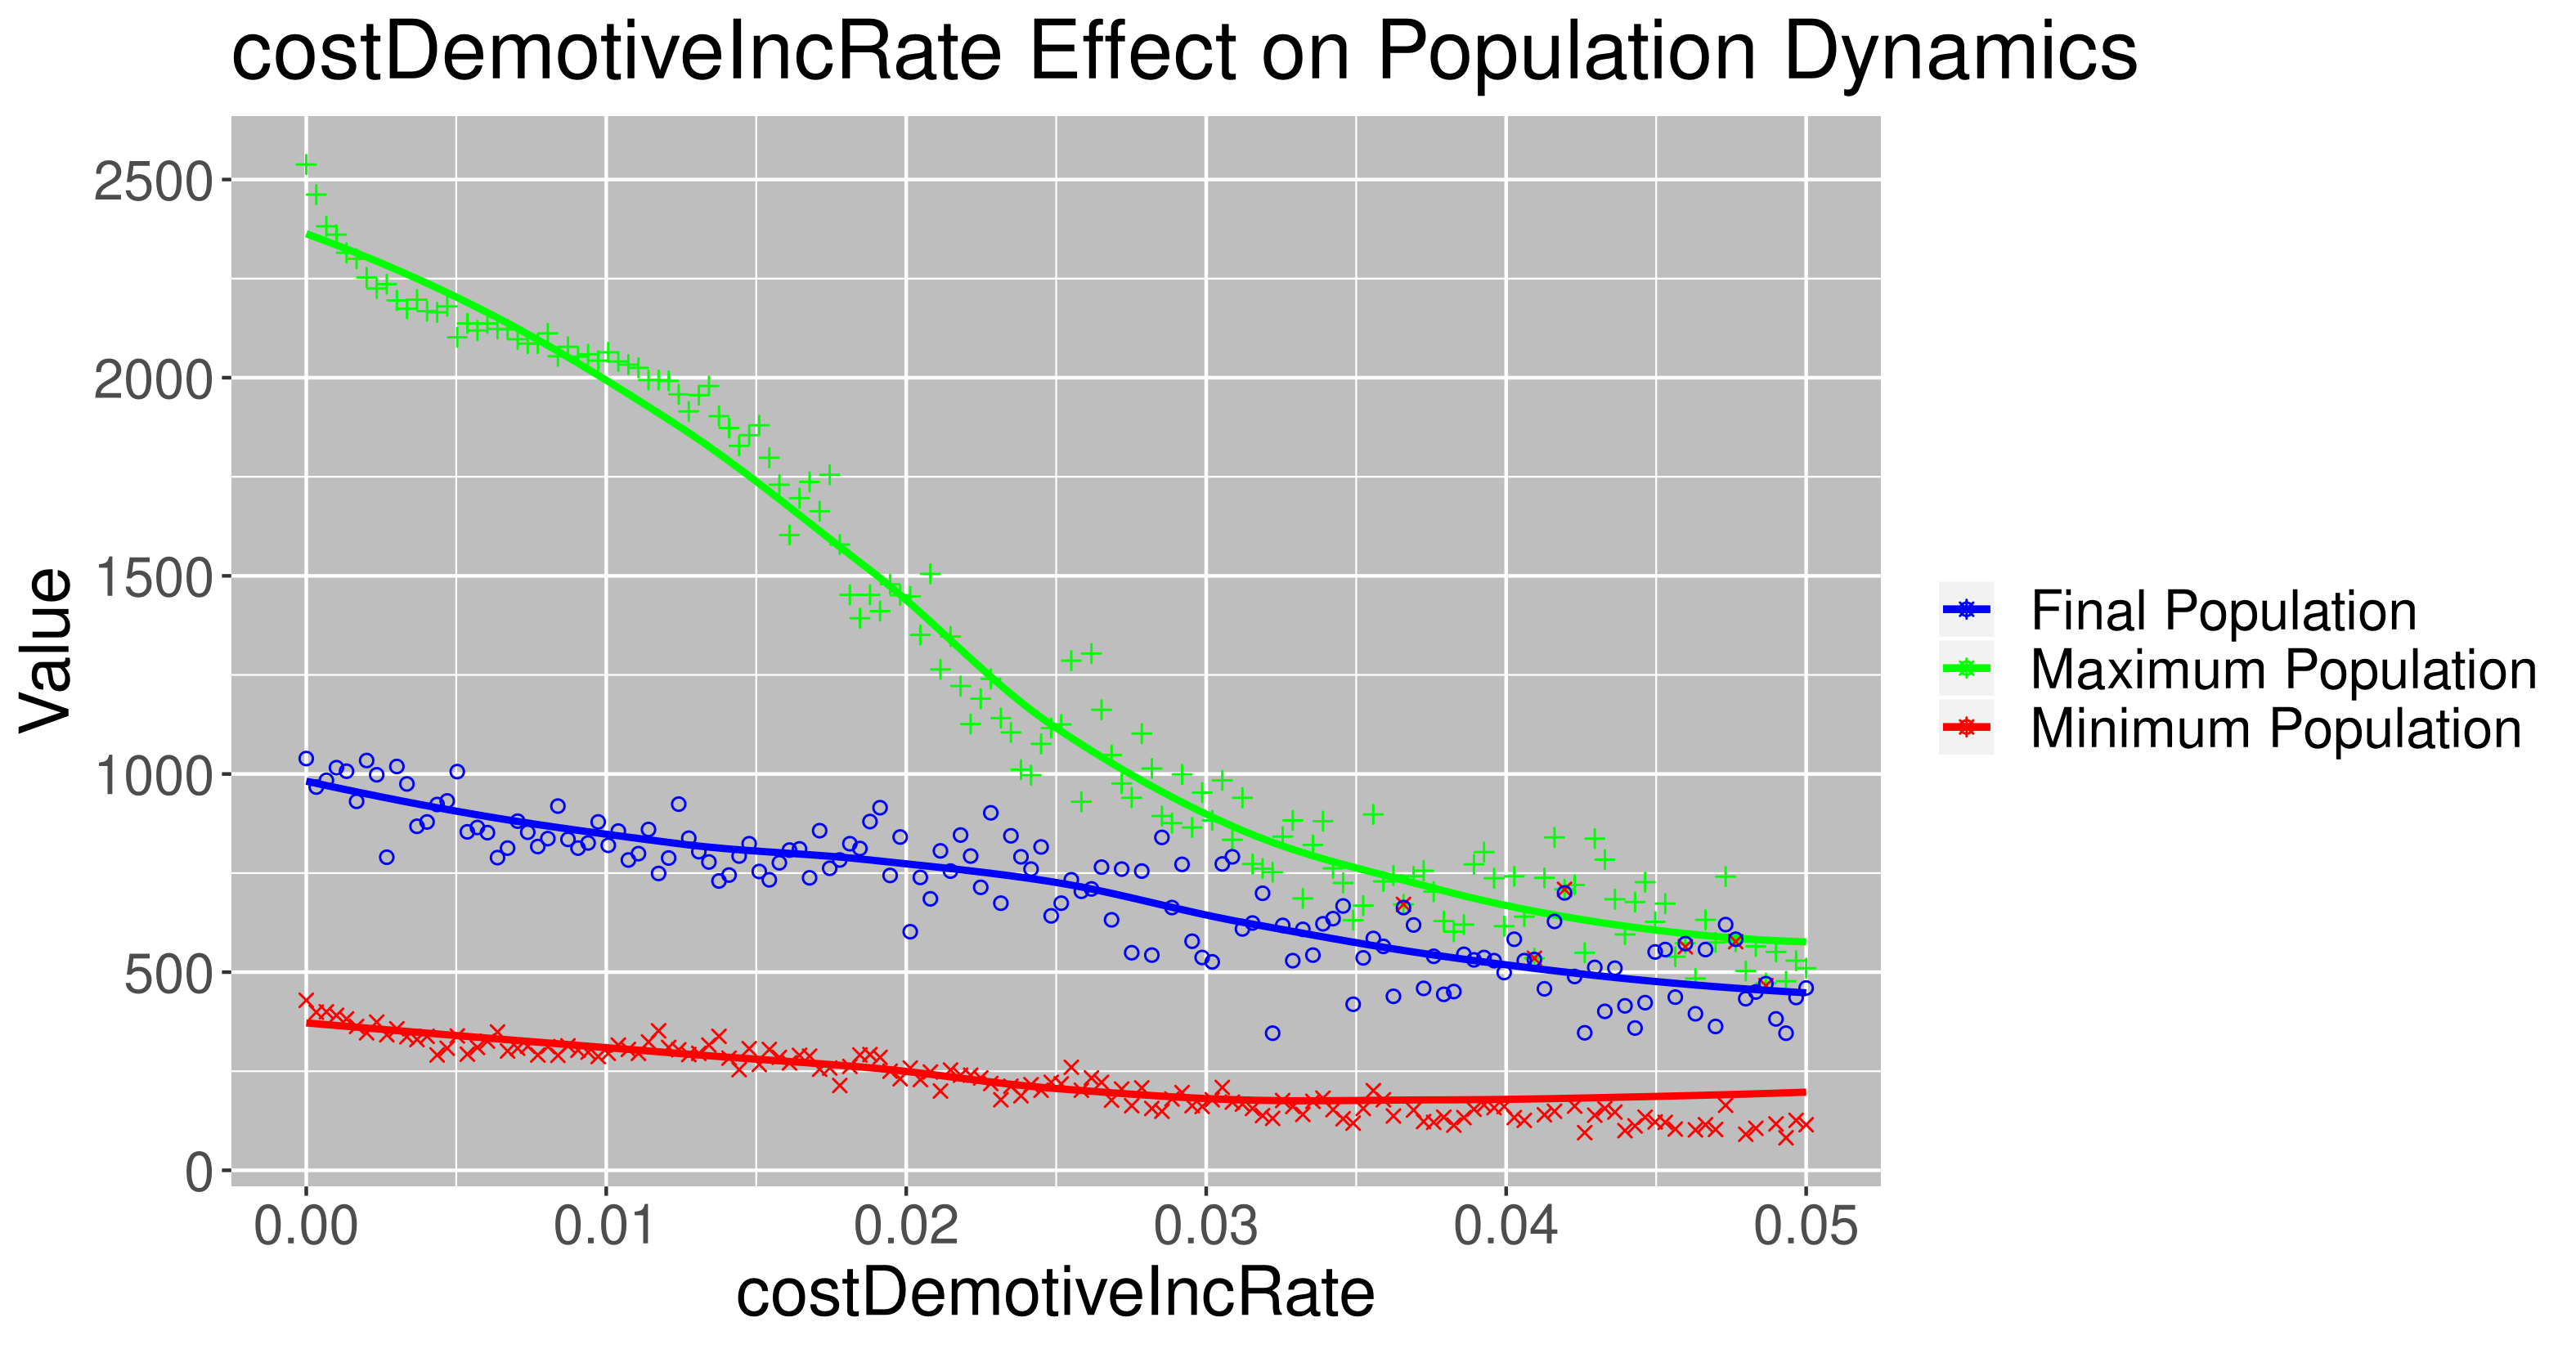
\includegraphics[width=5in]{/home/akara/workspace/R/CHAAHK/REPLACEME/figures/5-9}
	Plot corresponding to Figure 5.9 of Kara 2018
	\label{fig:5-9}
\end{figure}
\begin{figure}[H]
	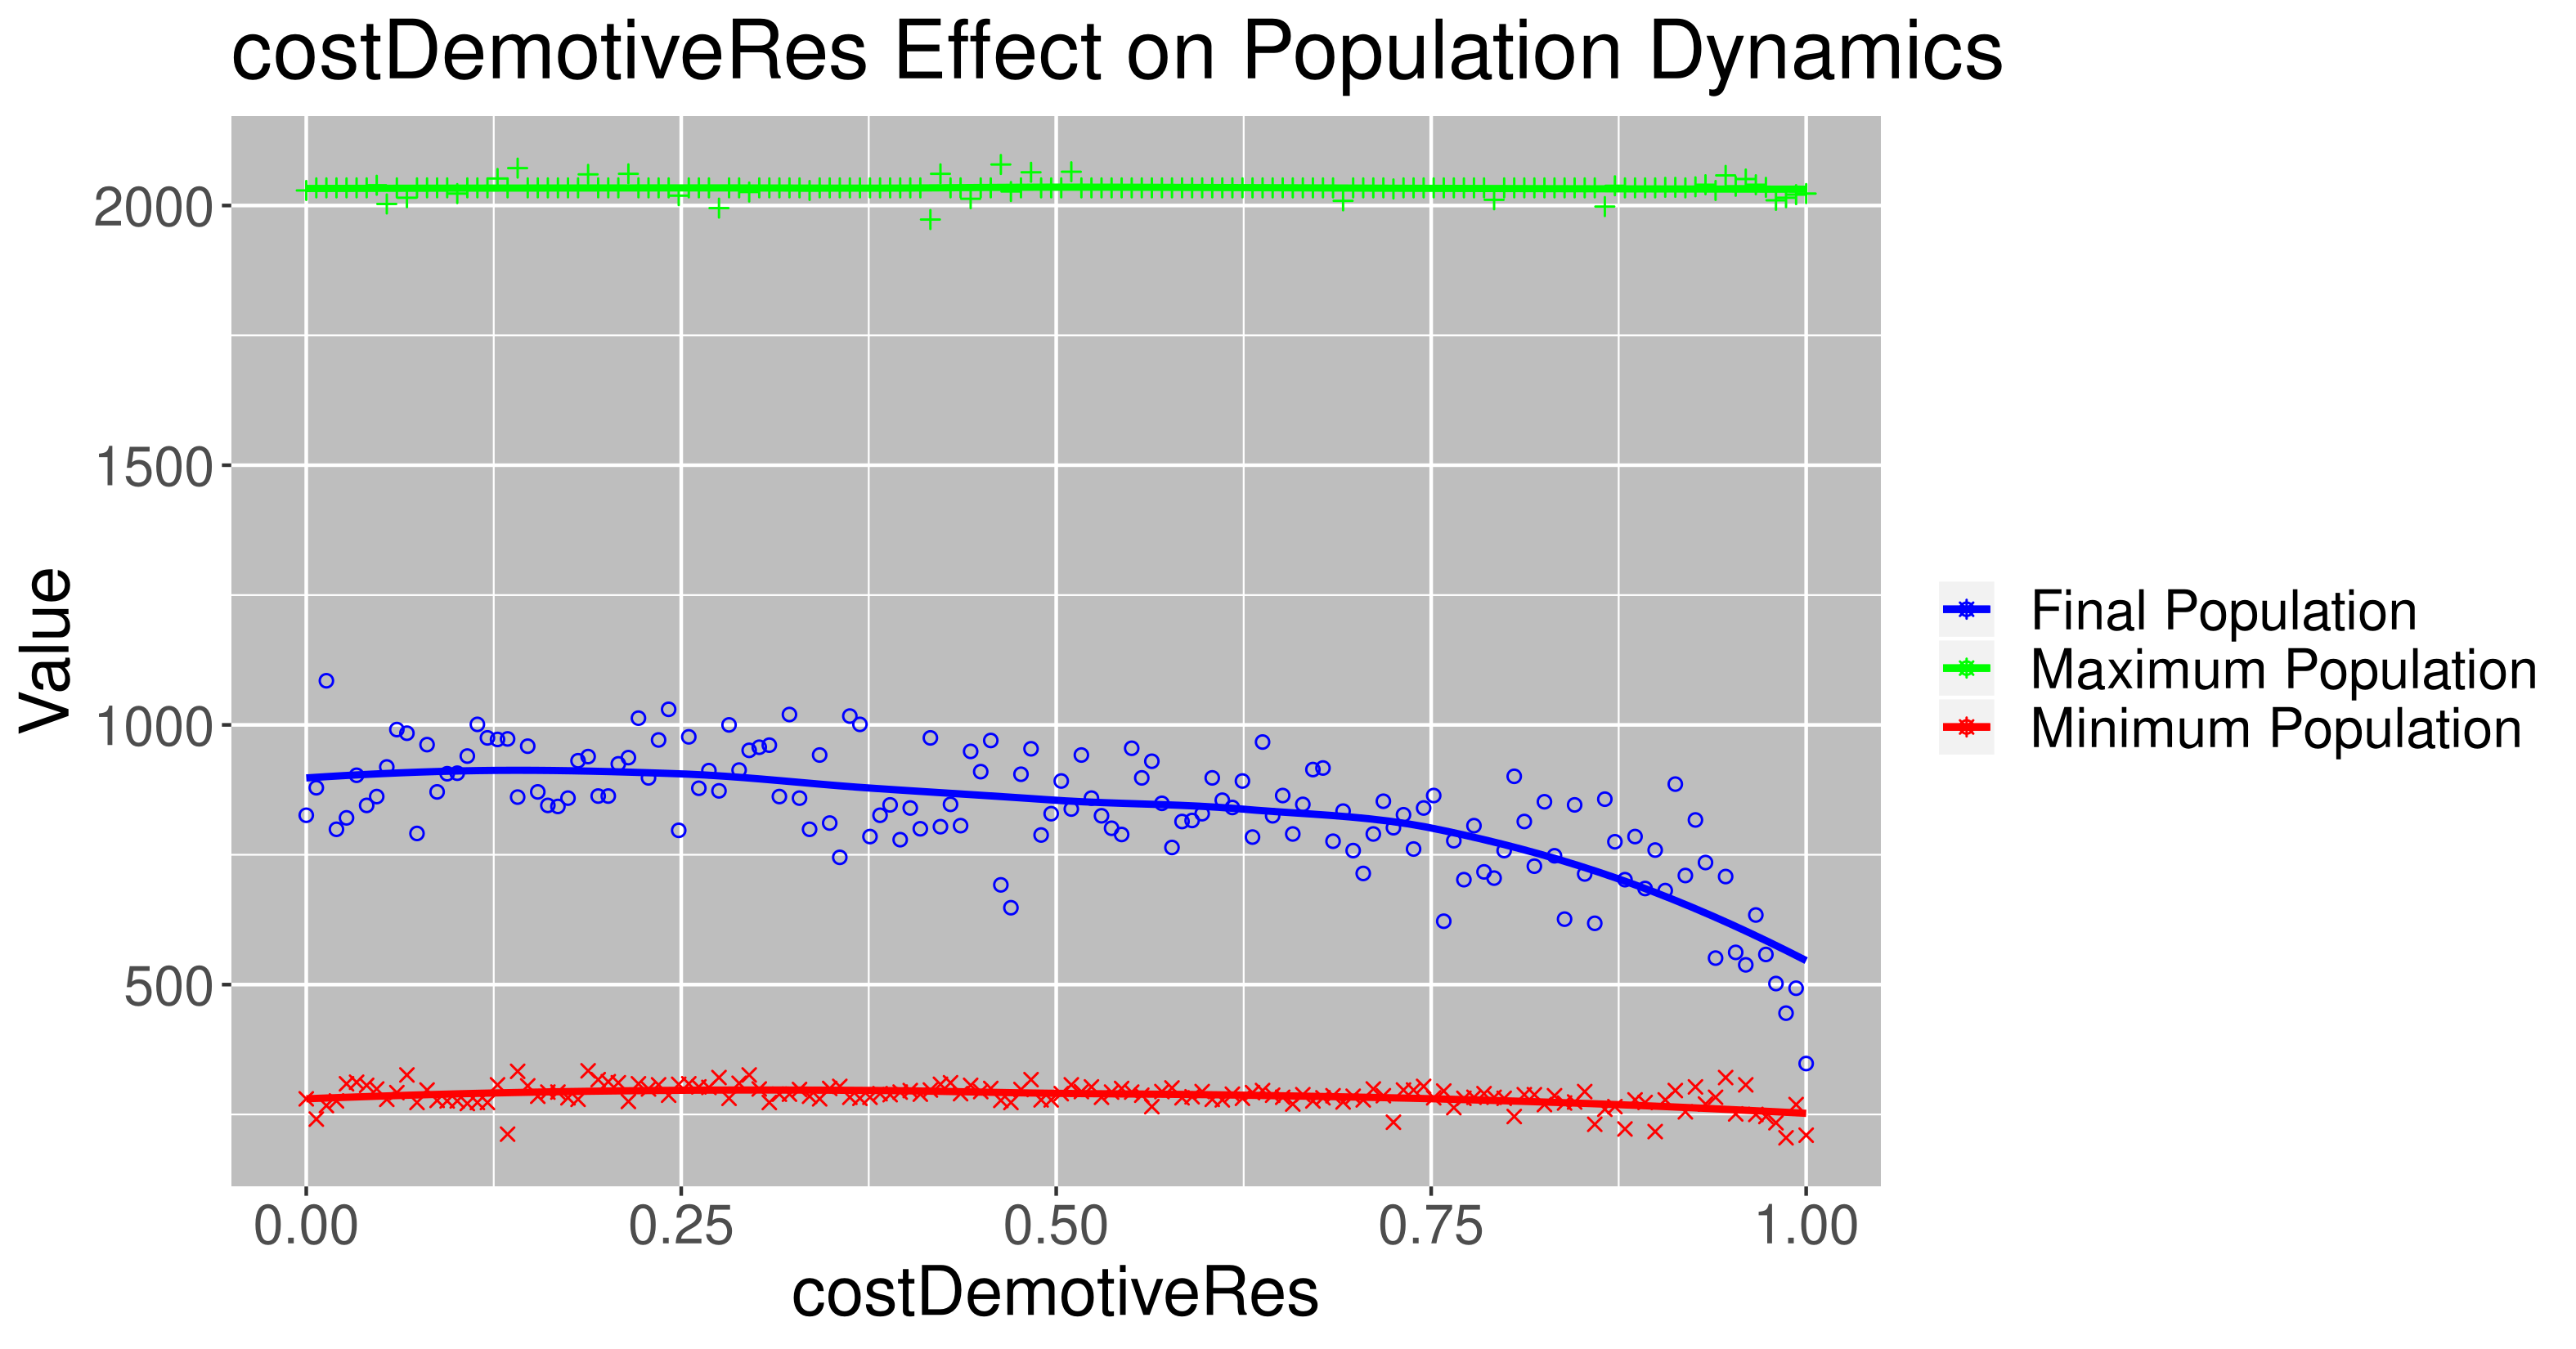
\includegraphics[width=5in]{/home/akara/workspace/R/CHAAHK/REPLACEME/figures/5-10}
	Plot corresponding to Figure 5.10 of Kara 2018
	\label{fig:5-10}
\end{figure}
\begin{figure}[H]
	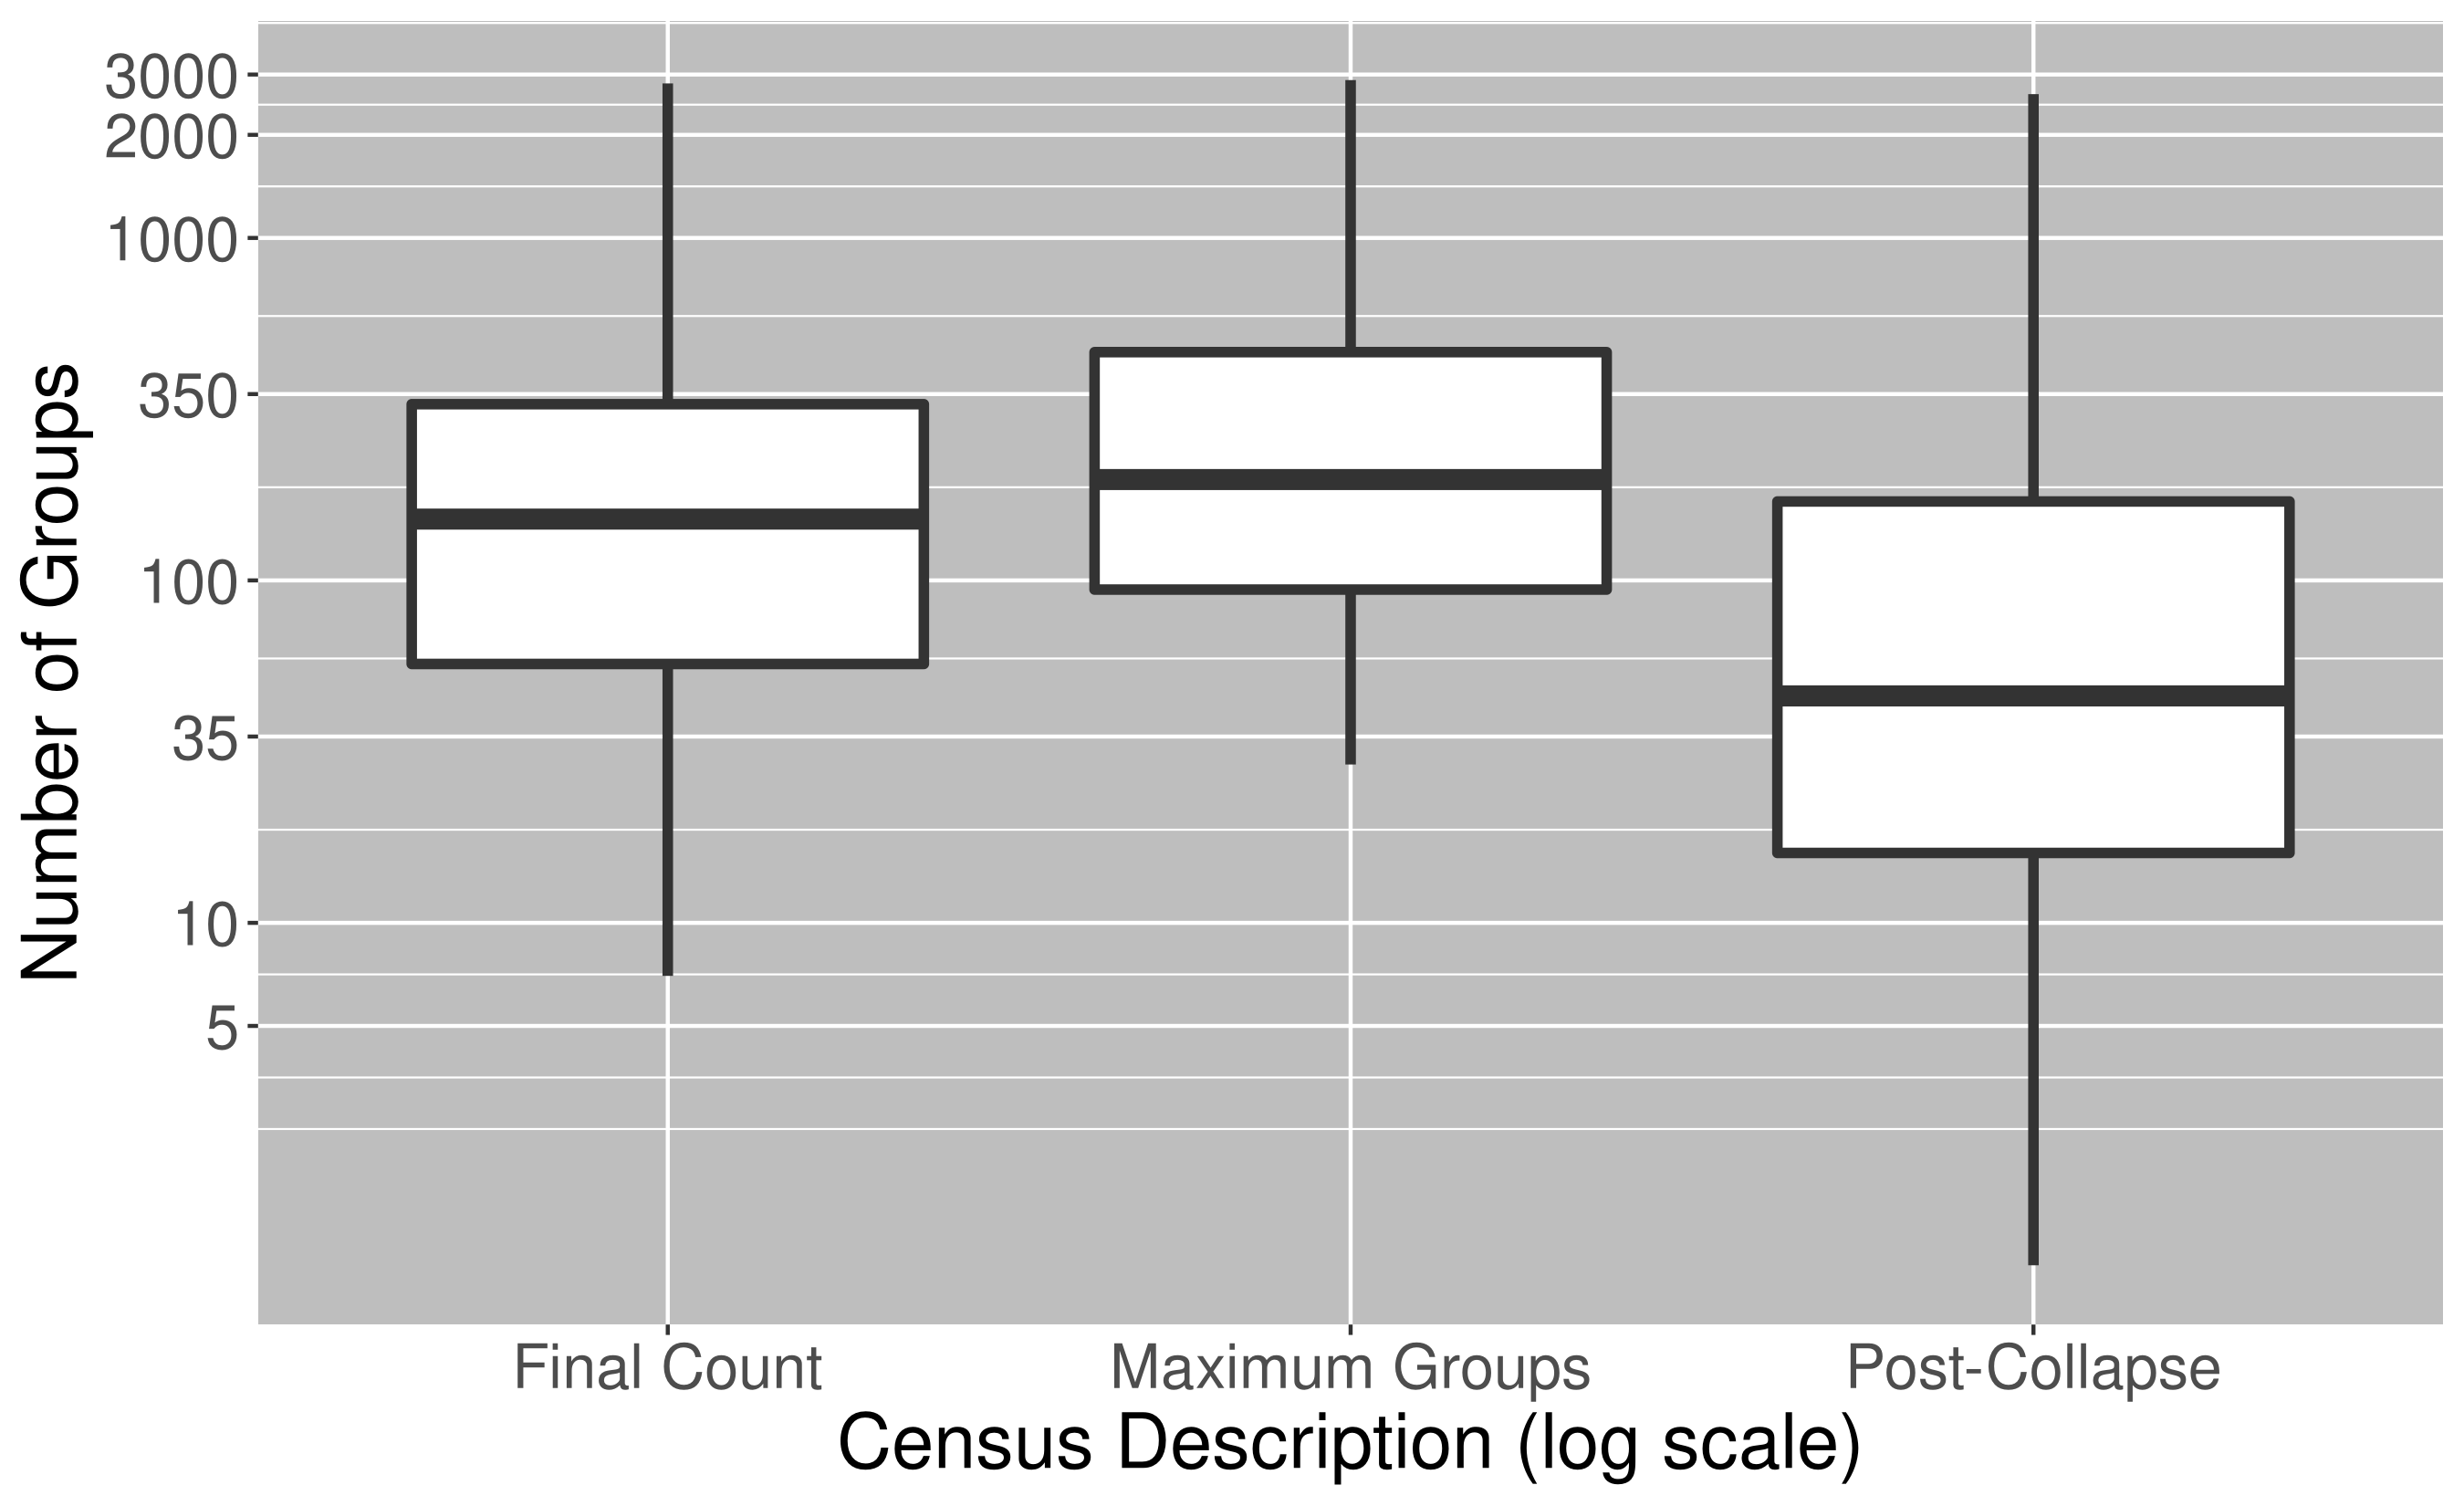
\includegraphics[width=5in]{/home/akara/workspace/R/CHAAHK/REPLACEME/figures/5-11}
	Plot corresponding to Figure 5.11 of Kara 2018
	\label{fig:5-11}
\end{figure}
\begin{figure}[H]
	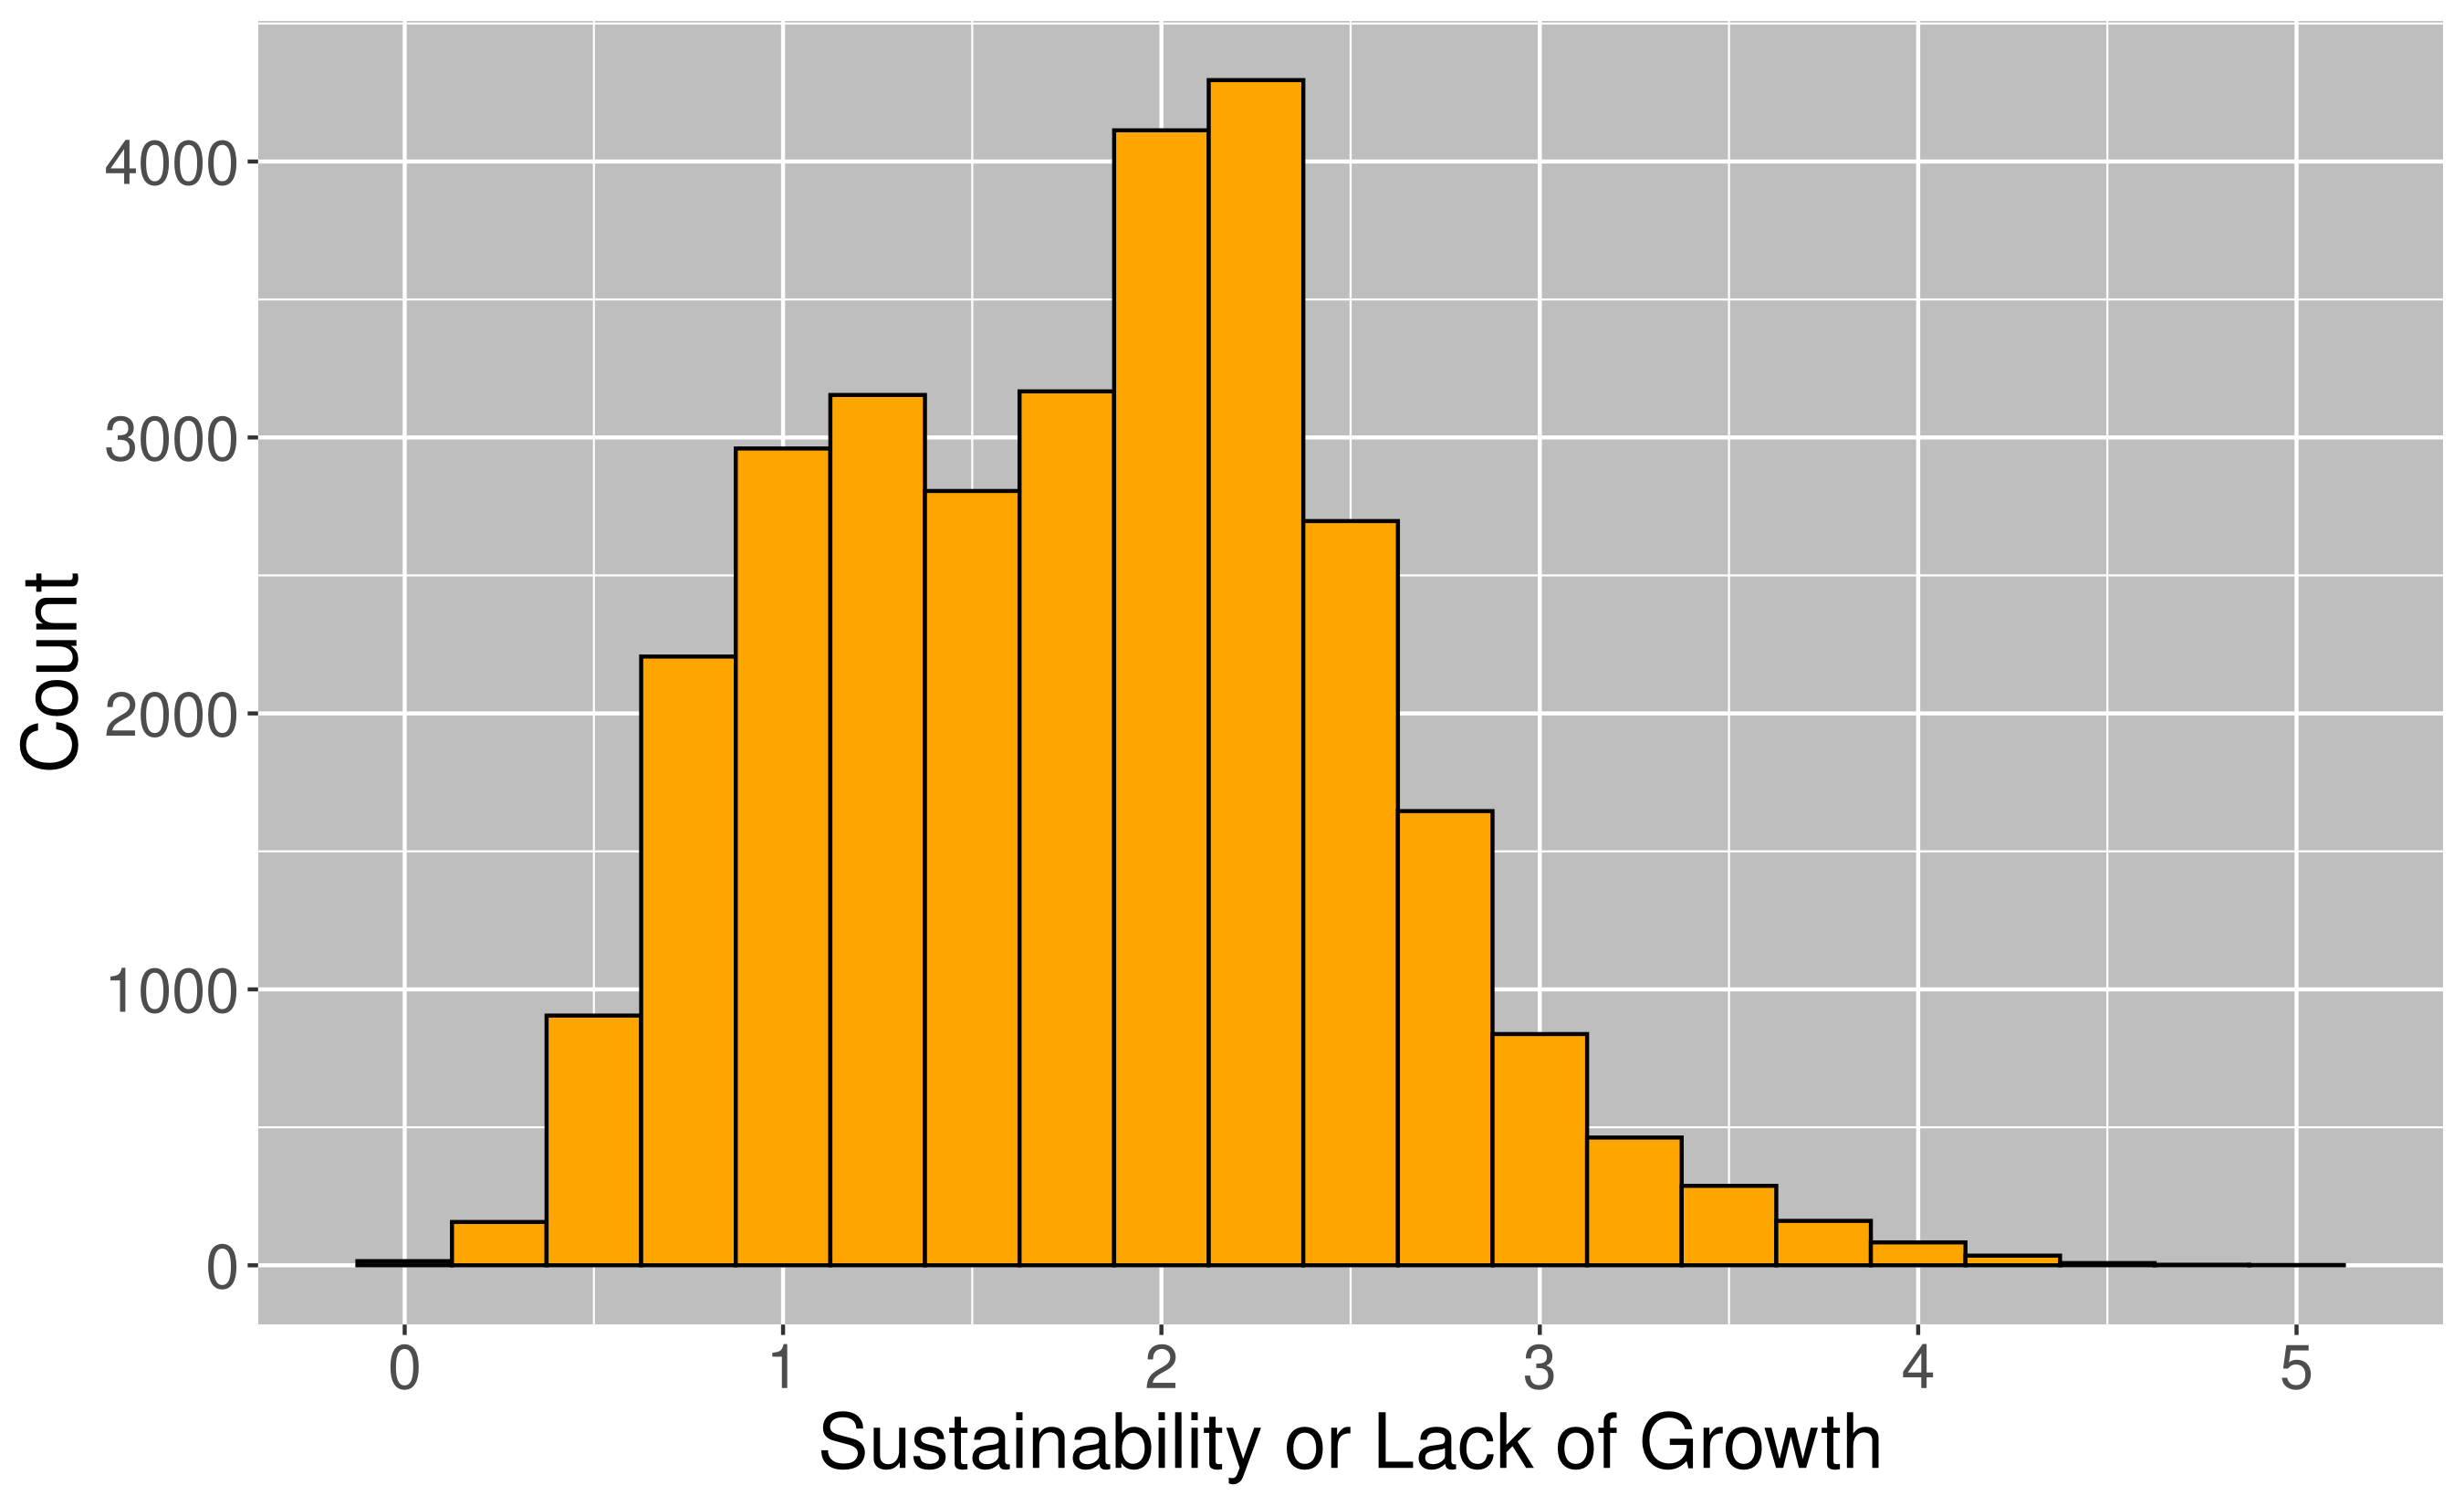
\includegraphics[width=5in]{/home/akara/workspace/R/CHAAHK/REPLACEME/figures/5-12}
	Plot corresponding to Figure 5.12 of Kara 2018
	\label{fig:5-12}
\end{figure}

\begin{table}[H]
\csvautotabular{/home/akara/workspace/R/CHAAHK/REPLACEME/tables/FOindices.csv}
\end{table}
\noindent Table of first order sensitivity indices corresponding to Table 5.2 of Kara 2018.

\begin{table}[H]
	\csvautotabular{/home/akara/workspace/R/CHAAHK/REPLACEME/tables/slopes.csv}
\end{table}
\noindent Table of multiple regression slopes associated with Table 5.3 of Kara 2018.

\begin{table}[H]
	\csvautotabular{/home/akara/workspace/R/CHAAHK/REPLACEME/tables/tvals.csv}
\end{table}
\noindent Table of multiple regression t values associated with Table 5.3 of Kara 2018.

\begin{table}[H]
	\csvautotabular{/home/akara/workspace/R/CHAAHK/REPLACEME/tables/Rsquares.csv}
\end{table}
\noindent Table of multiple regression R$ ^{2} $ values associated with Table 5.3 of Kara 2018.
\newline
\begin{table}[H]
	\csvautotabular{/home/akara/workspace/R/CHAAHK/REPLACEME/tables/TreeImportance.csv}
\end{table}
\noindent Table variable importance corresponding to Table 5.4 of Kara 2018.
\begin{sidewaysfigure}
	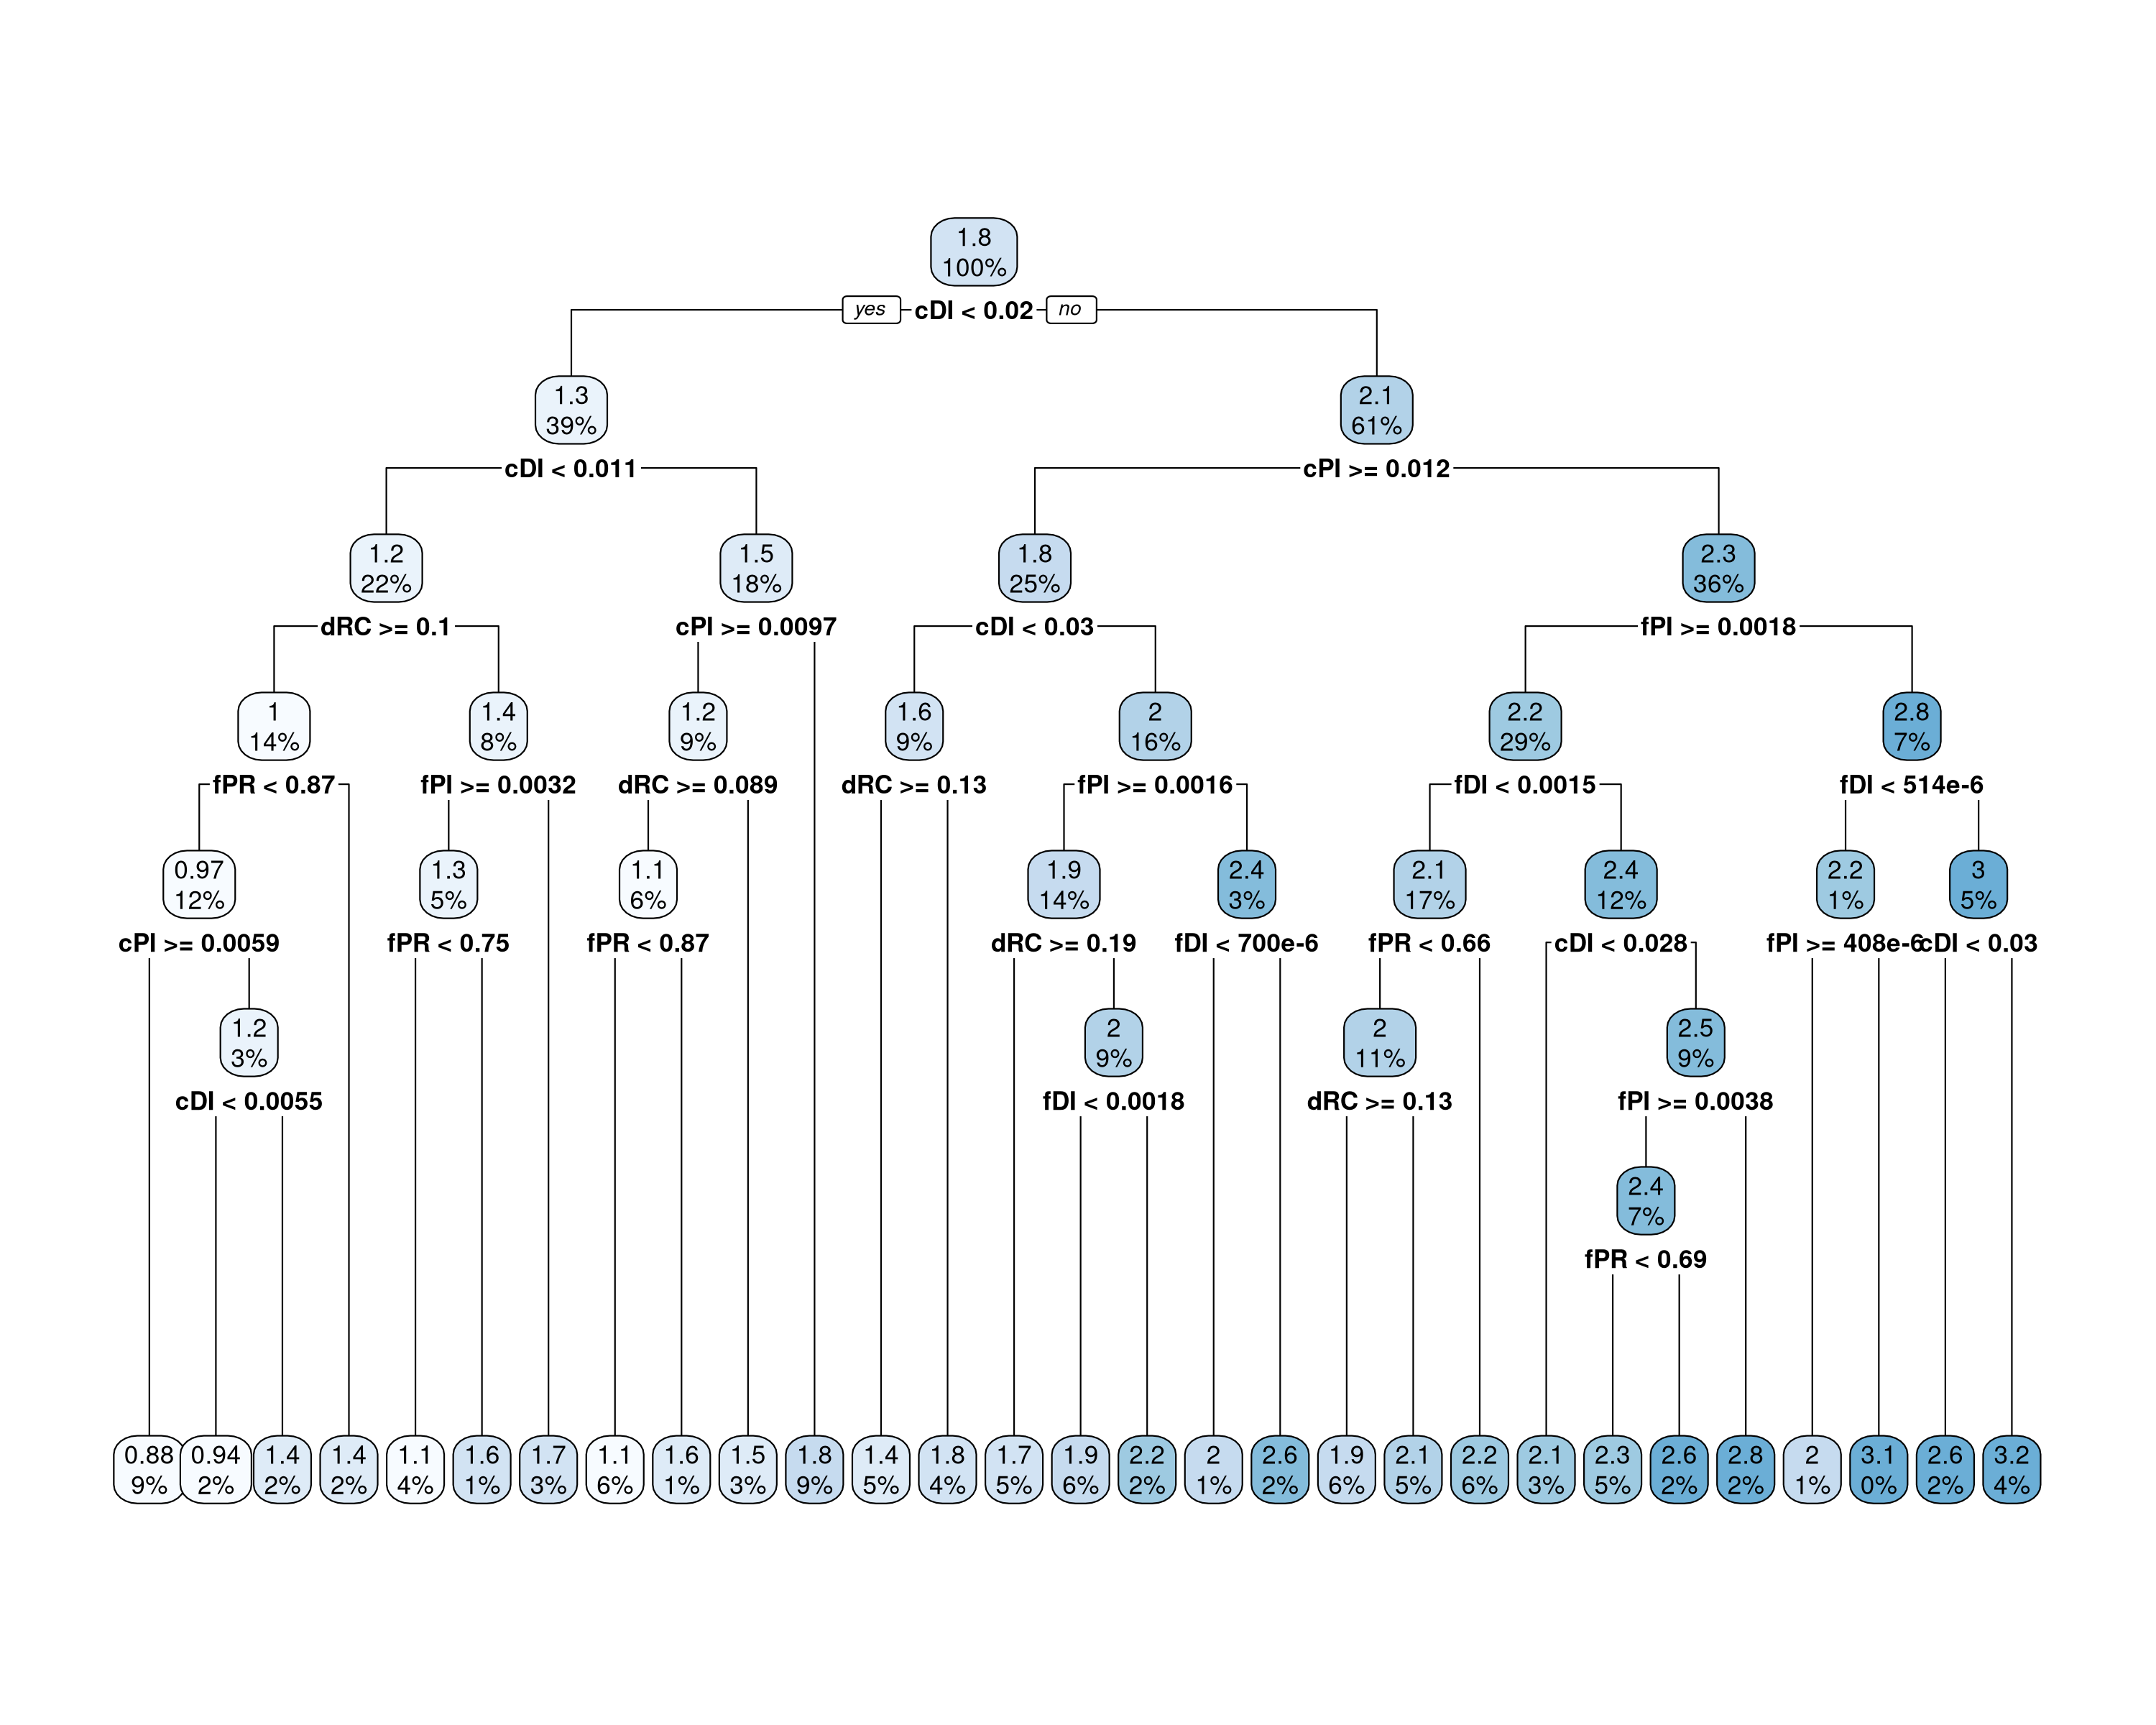
\includegraphics[width=8in]{/home/akara/workspace/R/CHAAHK/REPLACEME/figures/5-13-14-15-16}
	\caption{Plot corresponding to Figures 5.13, 5.14, 5.15, and 5.16 of Kara 2018}
	\label{fig:5-13-16}
\end{sidewaysfigure}
\begin{figure}[H]
	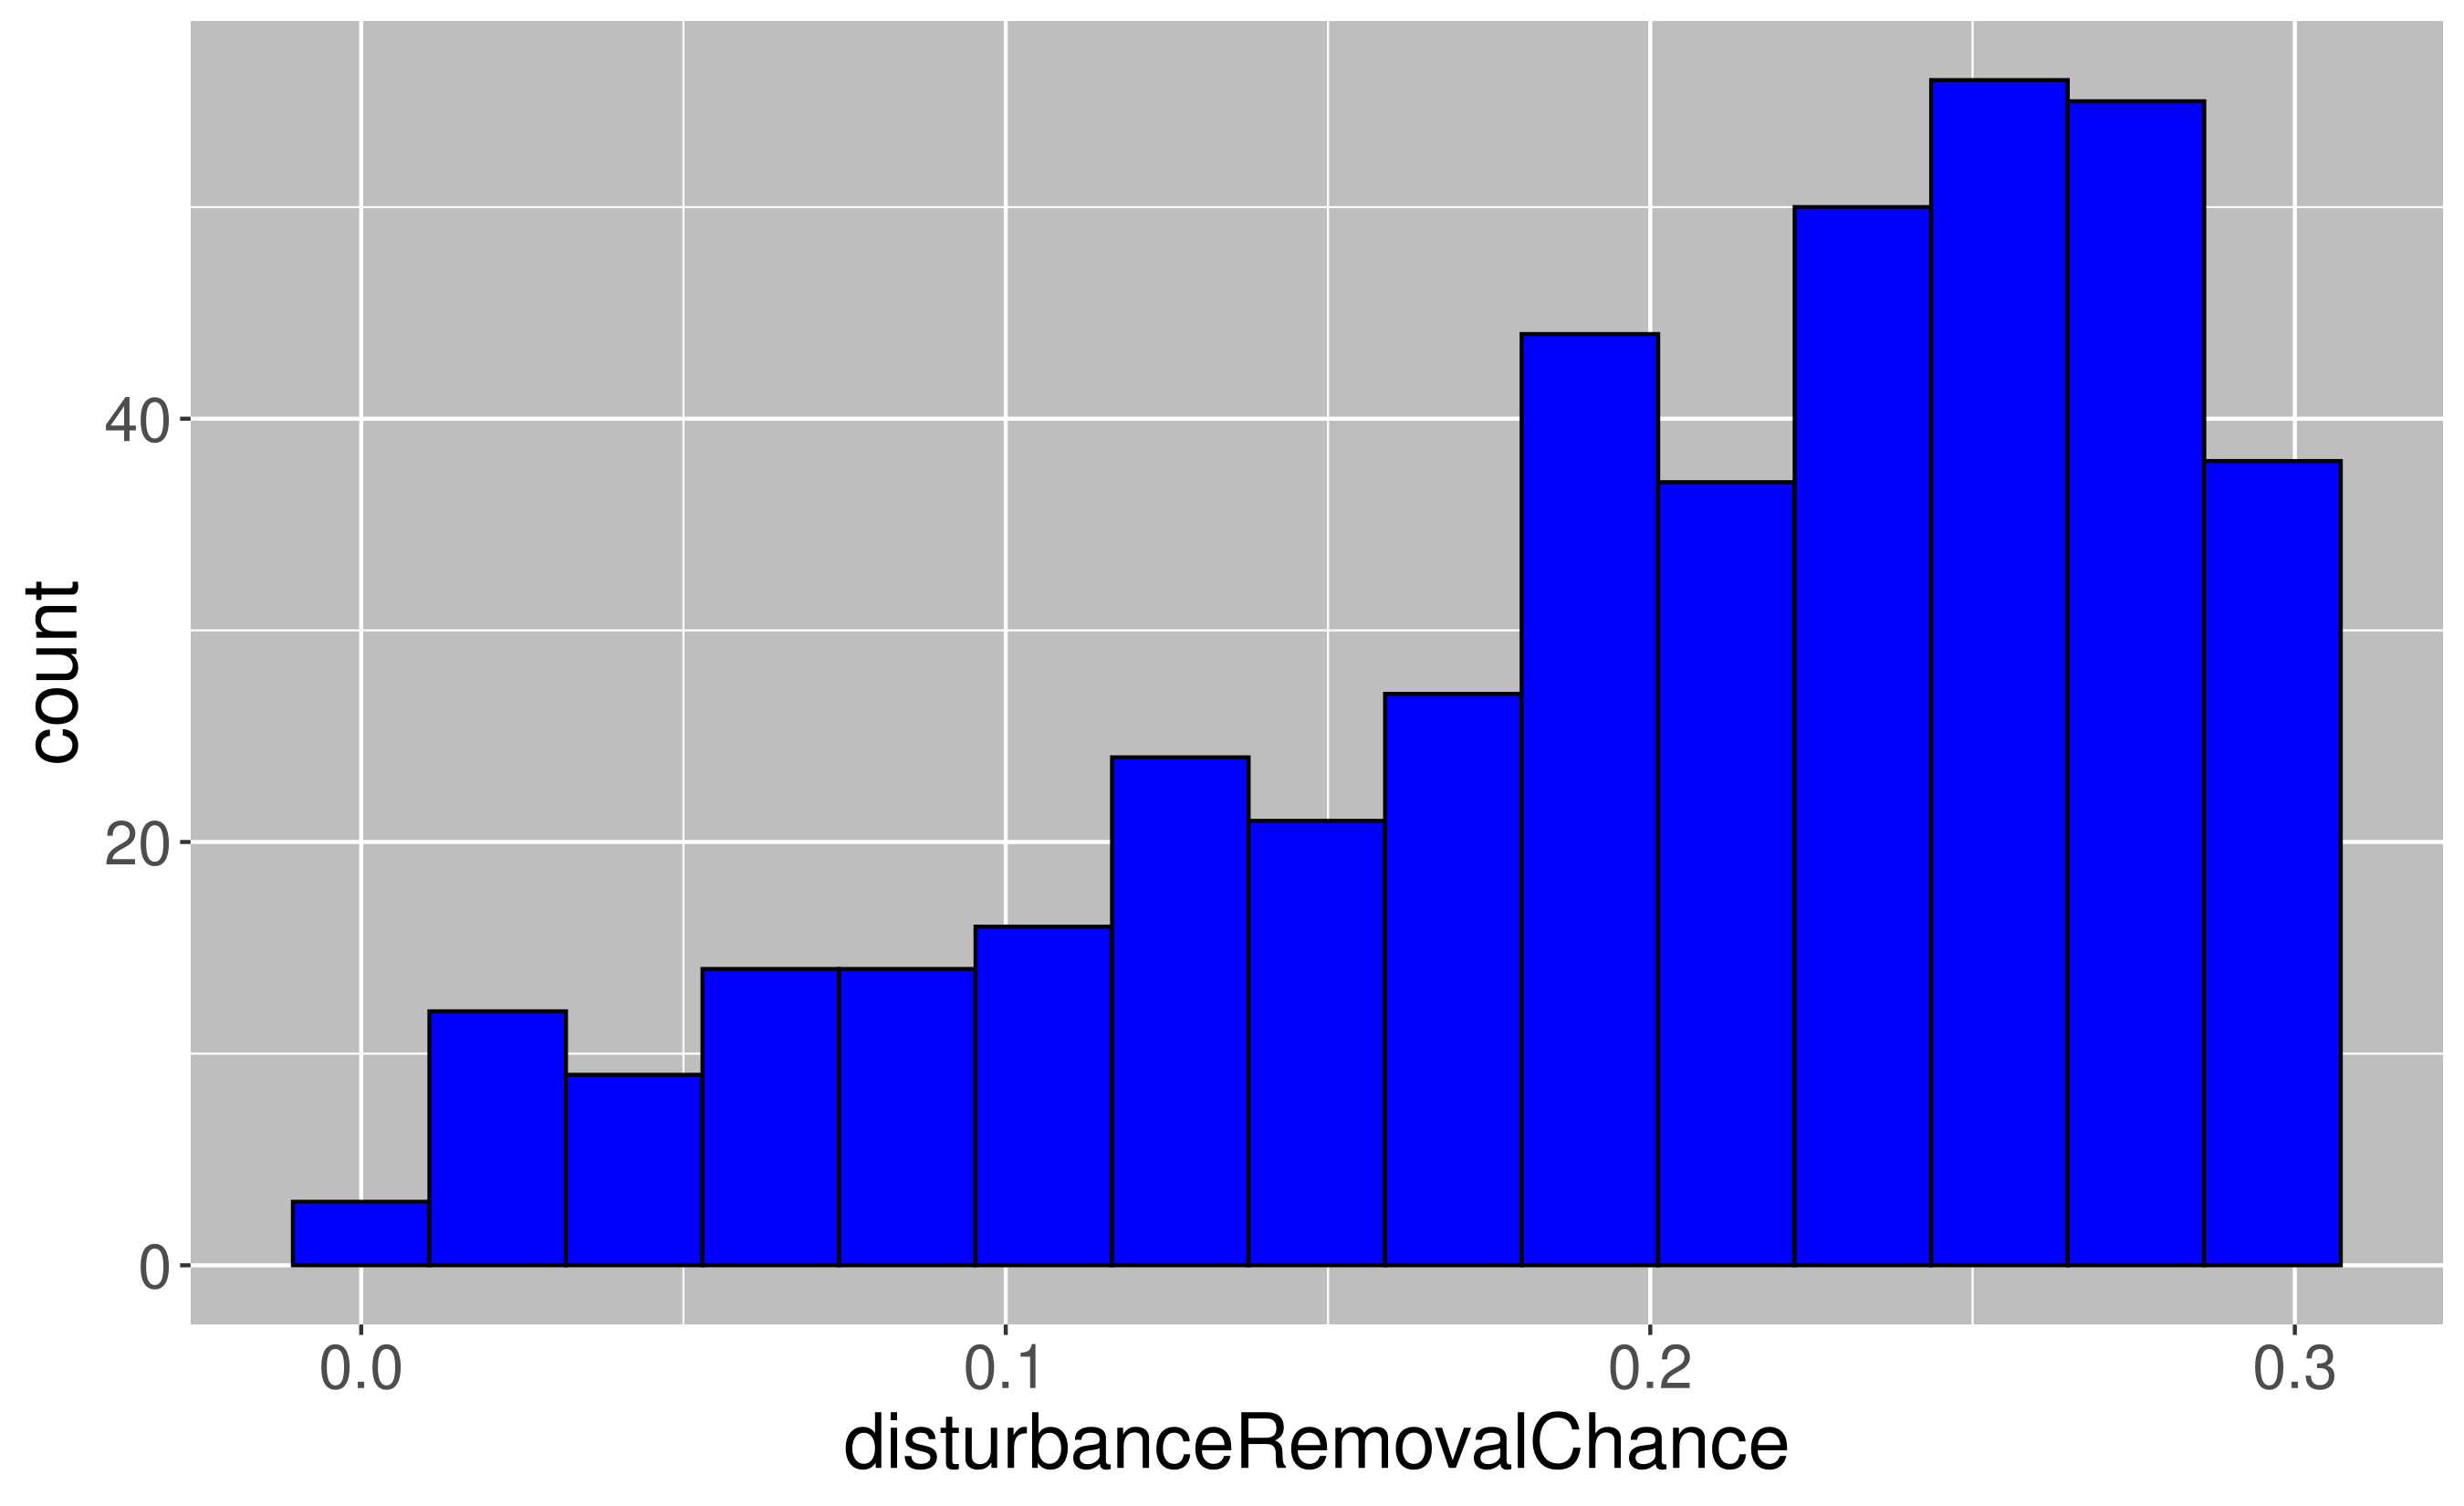
\includegraphics[width=5in]{/home/akara/workspace/R/CHAAHK/REPLACEME/figures/5-18}
	Plot corresponding to Figure 5.18 of Kara 2018
	\label{fig:5-18}
\end{figure}
\begin{figure}[H]
	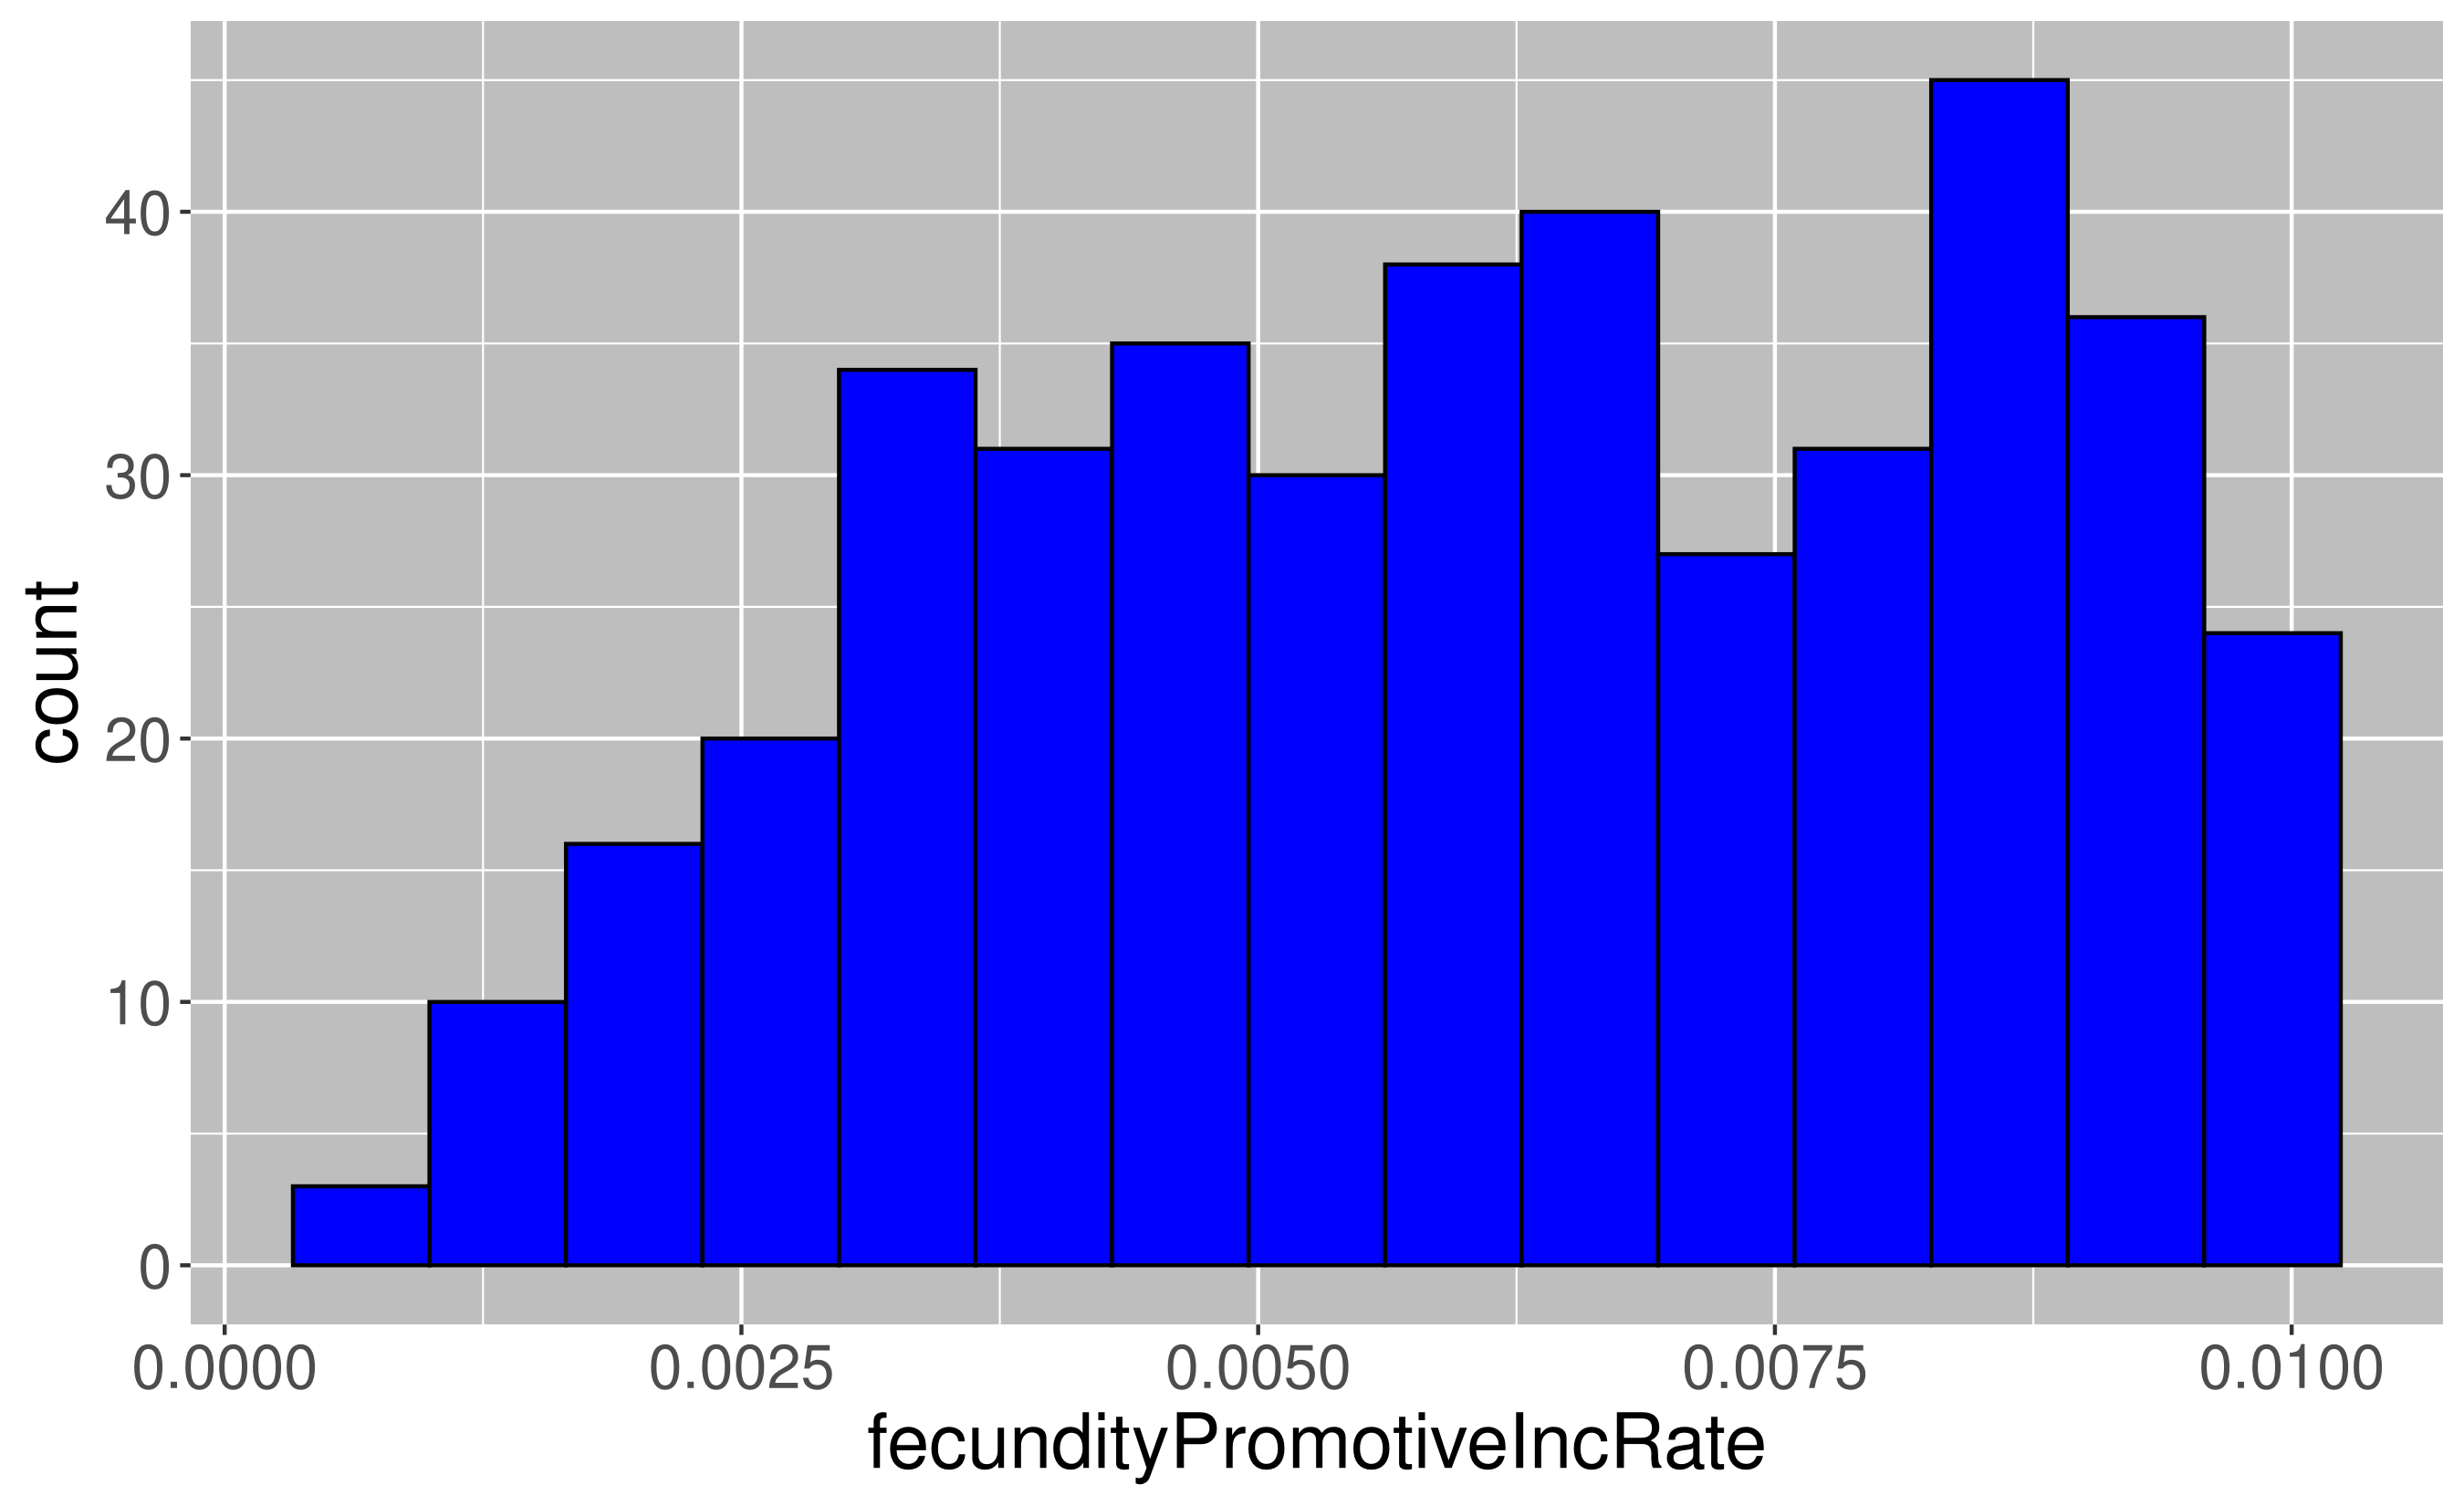
\includegraphics[width=5in]{/home/akara/workspace/R/CHAAHK/REPLACEME/figures/5-19}
	Plot corresponding to Figure 5.19 of Kara 2018
	\label{fig:5-19}
\end{figure}
\begin{figure}[H]
	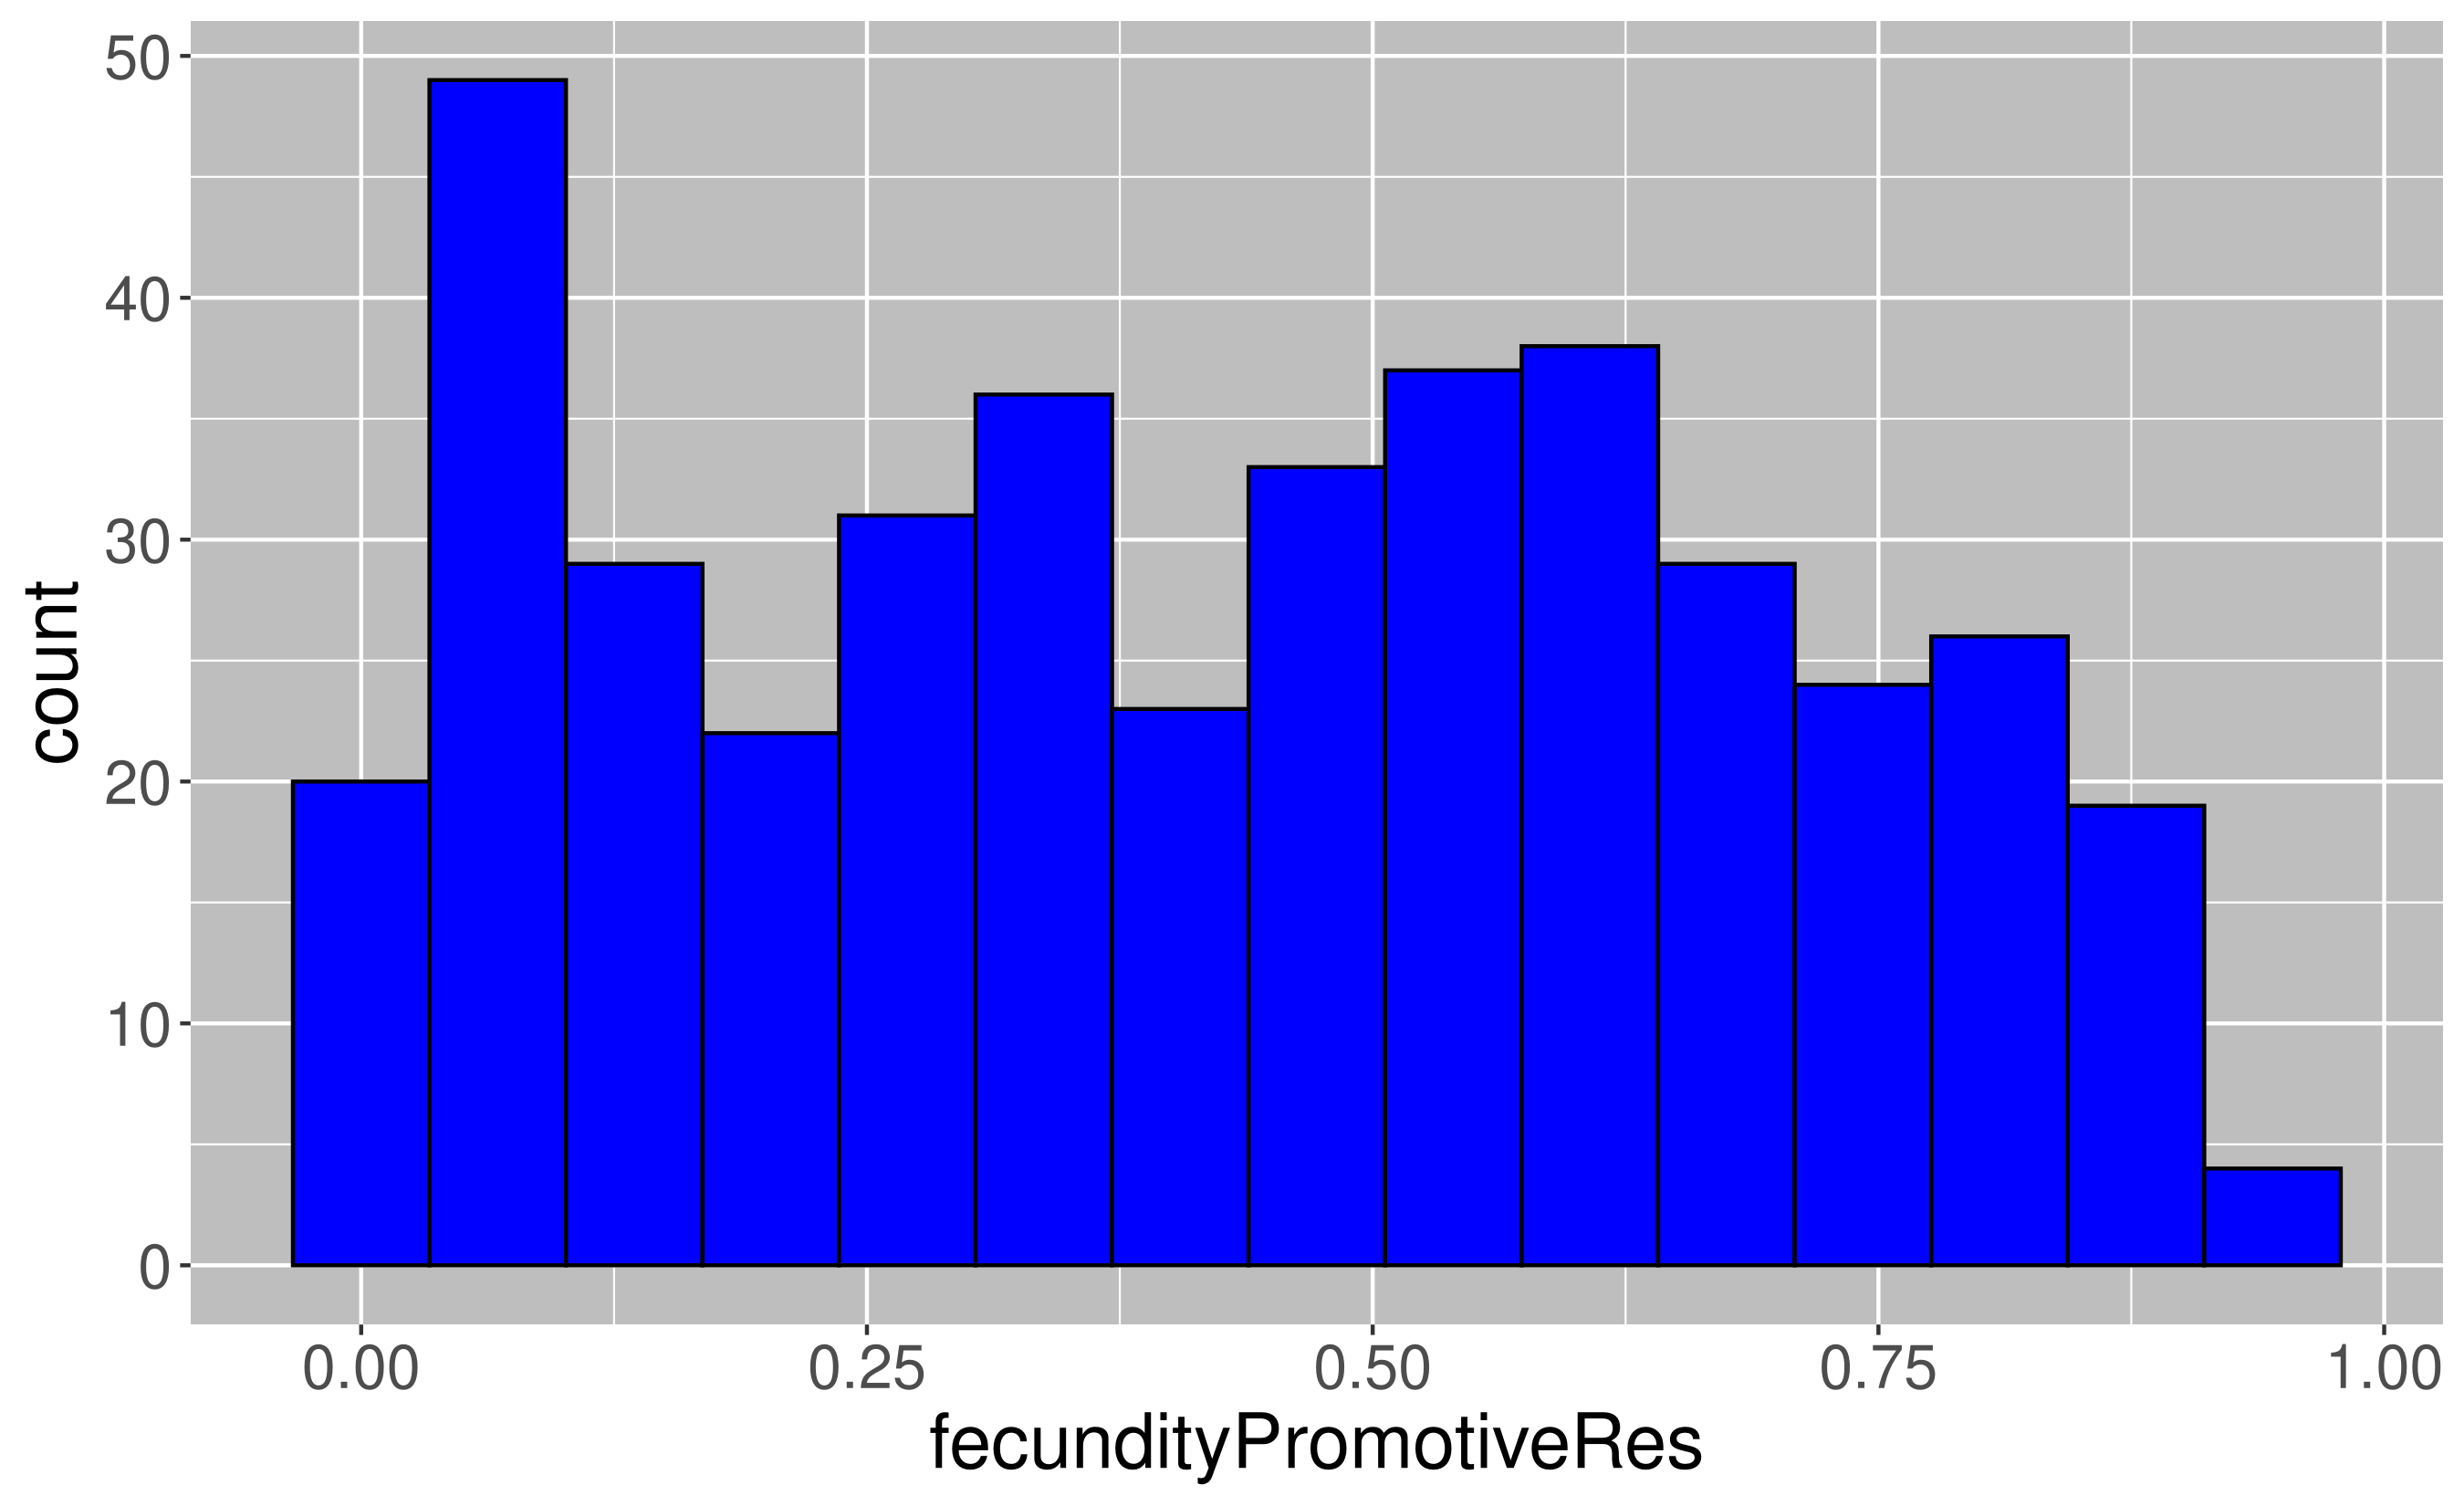
\includegraphics[width=5in]{/home/akara/workspace/R/CHAAHK/REPLACEME/figures/5-20}
	Plot corresponding to Figure 5.20 of Kara 2018
	\label{fig:5-20}
\end{figure}
\begin{figure}[H]
	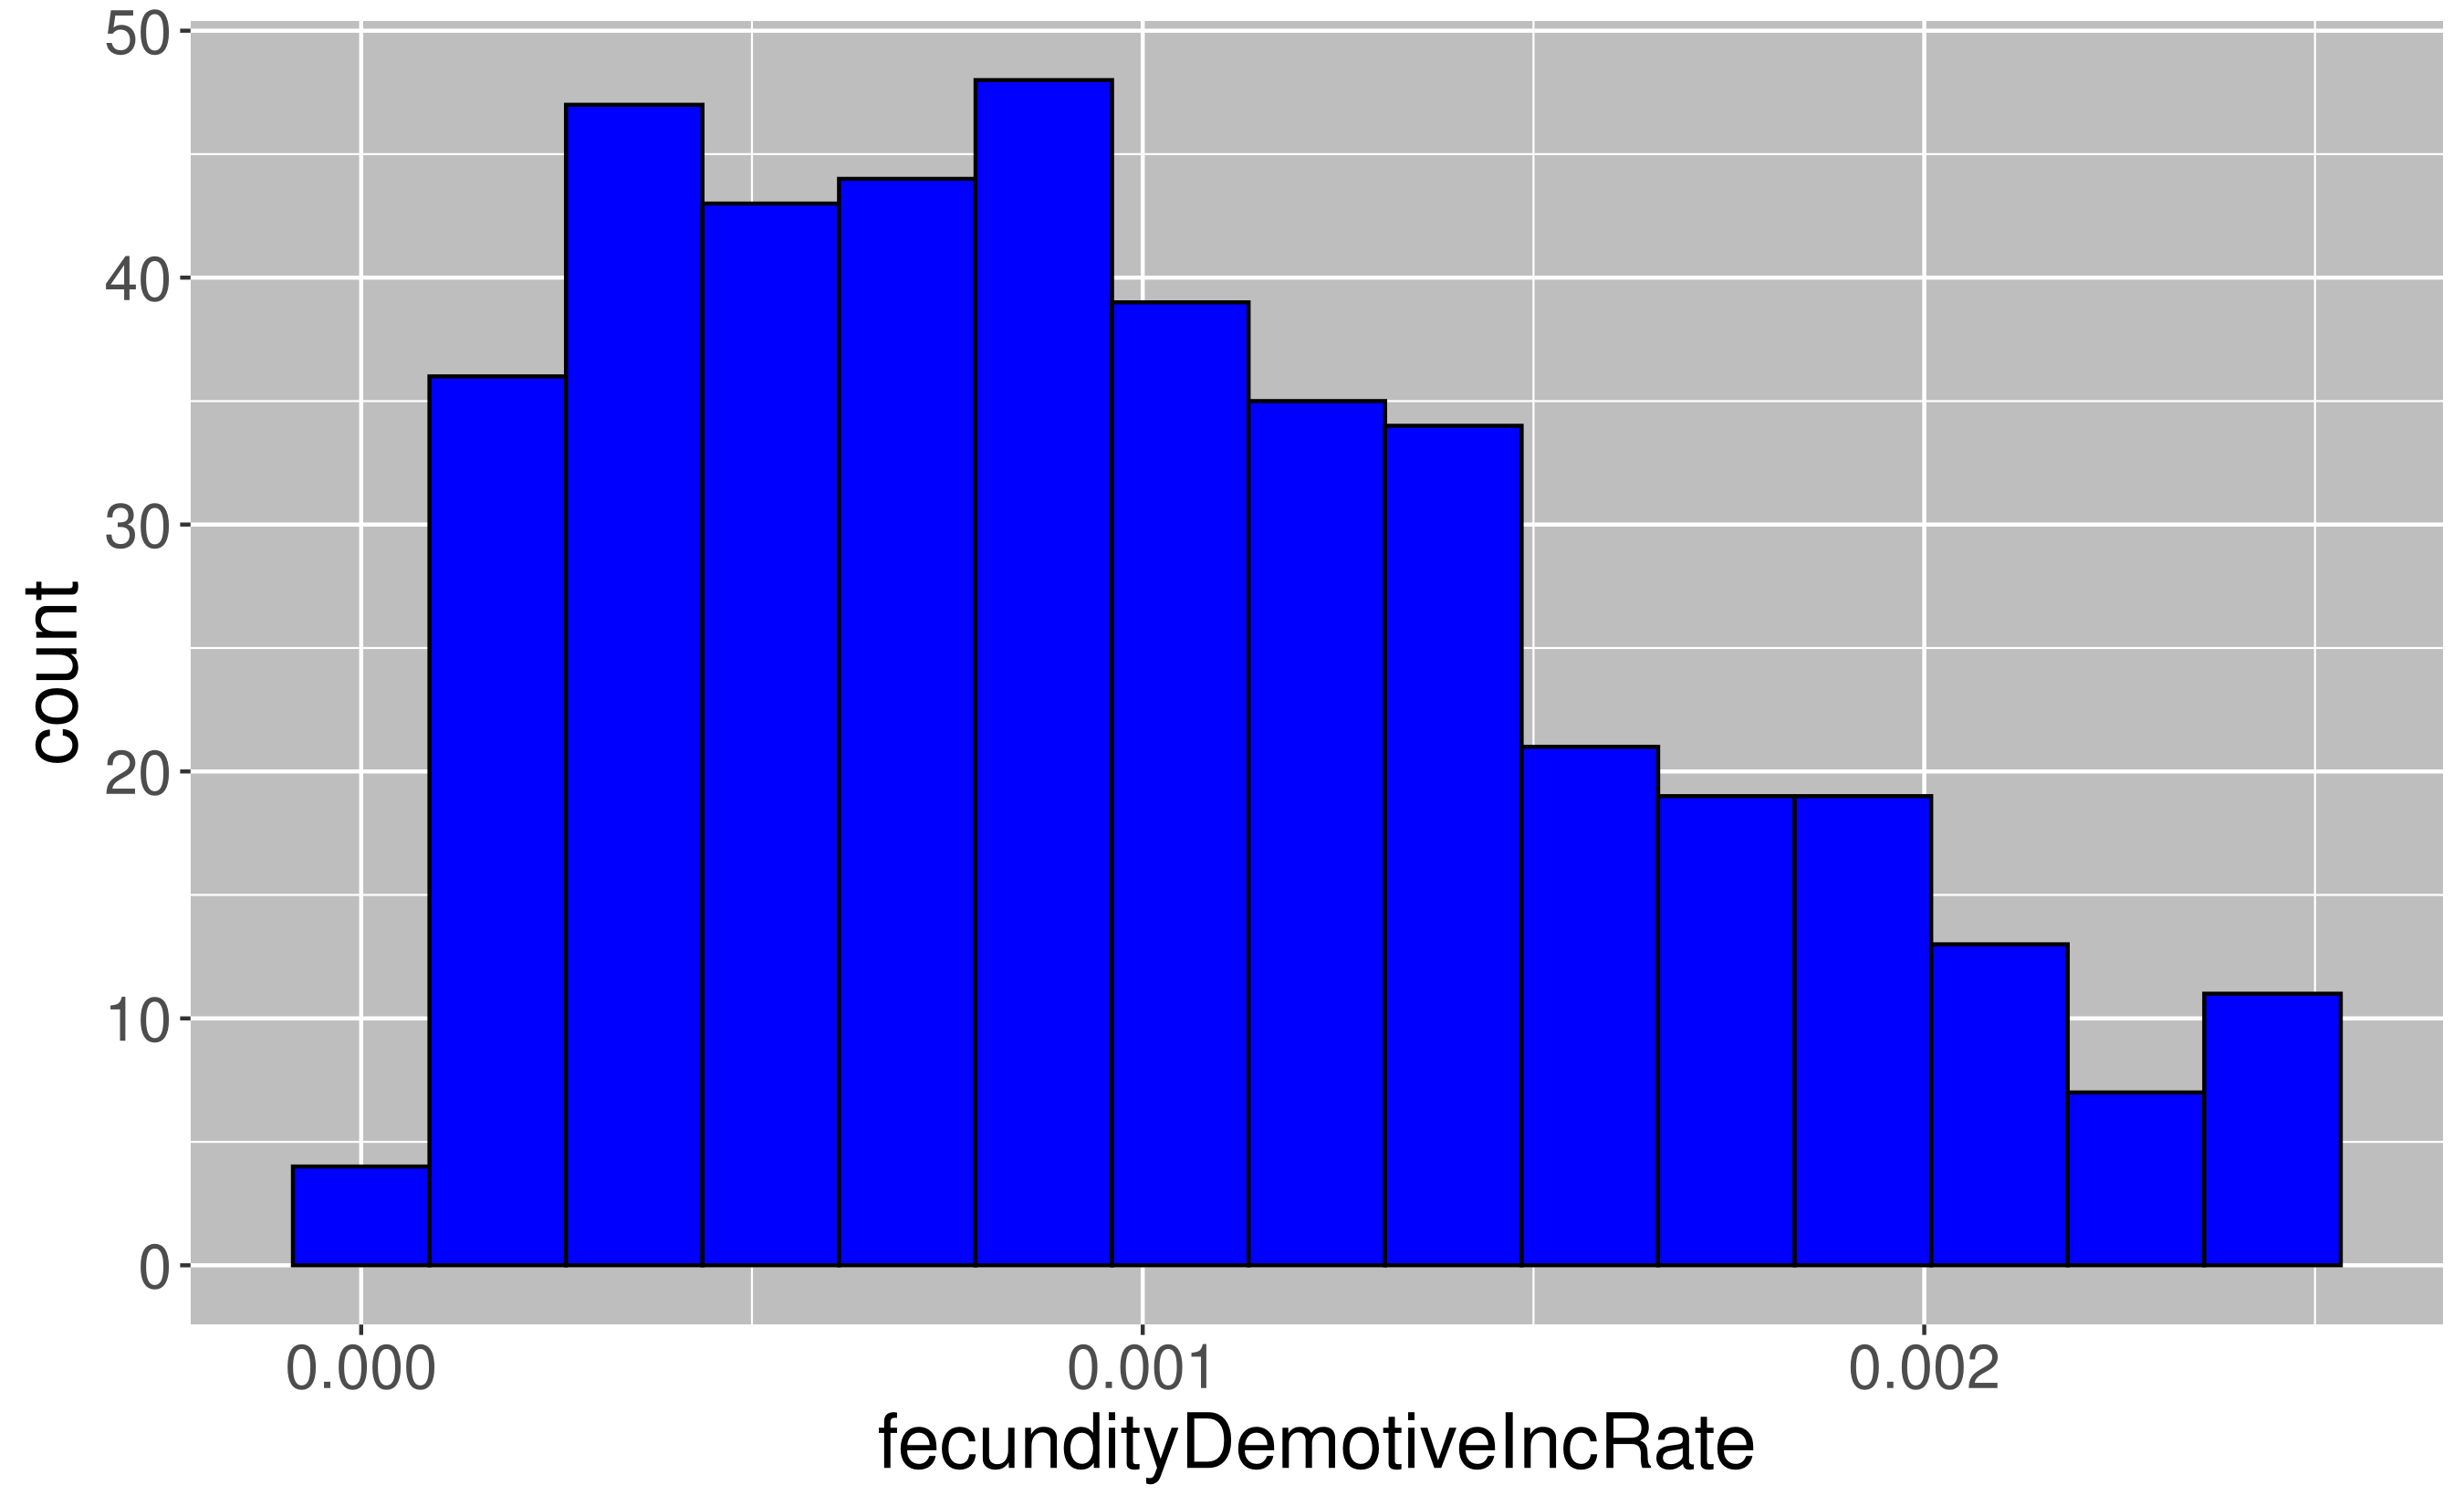
\includegraphics[width=5in]{/home/akara/workspace/R/CHAAHK/REPLACEME/figures/5-21}
	Plot corresponding to Figure 5.21 of Kara 2018
	\label{fig:5-21}
\end{figure}
\begin{figure}[H]
	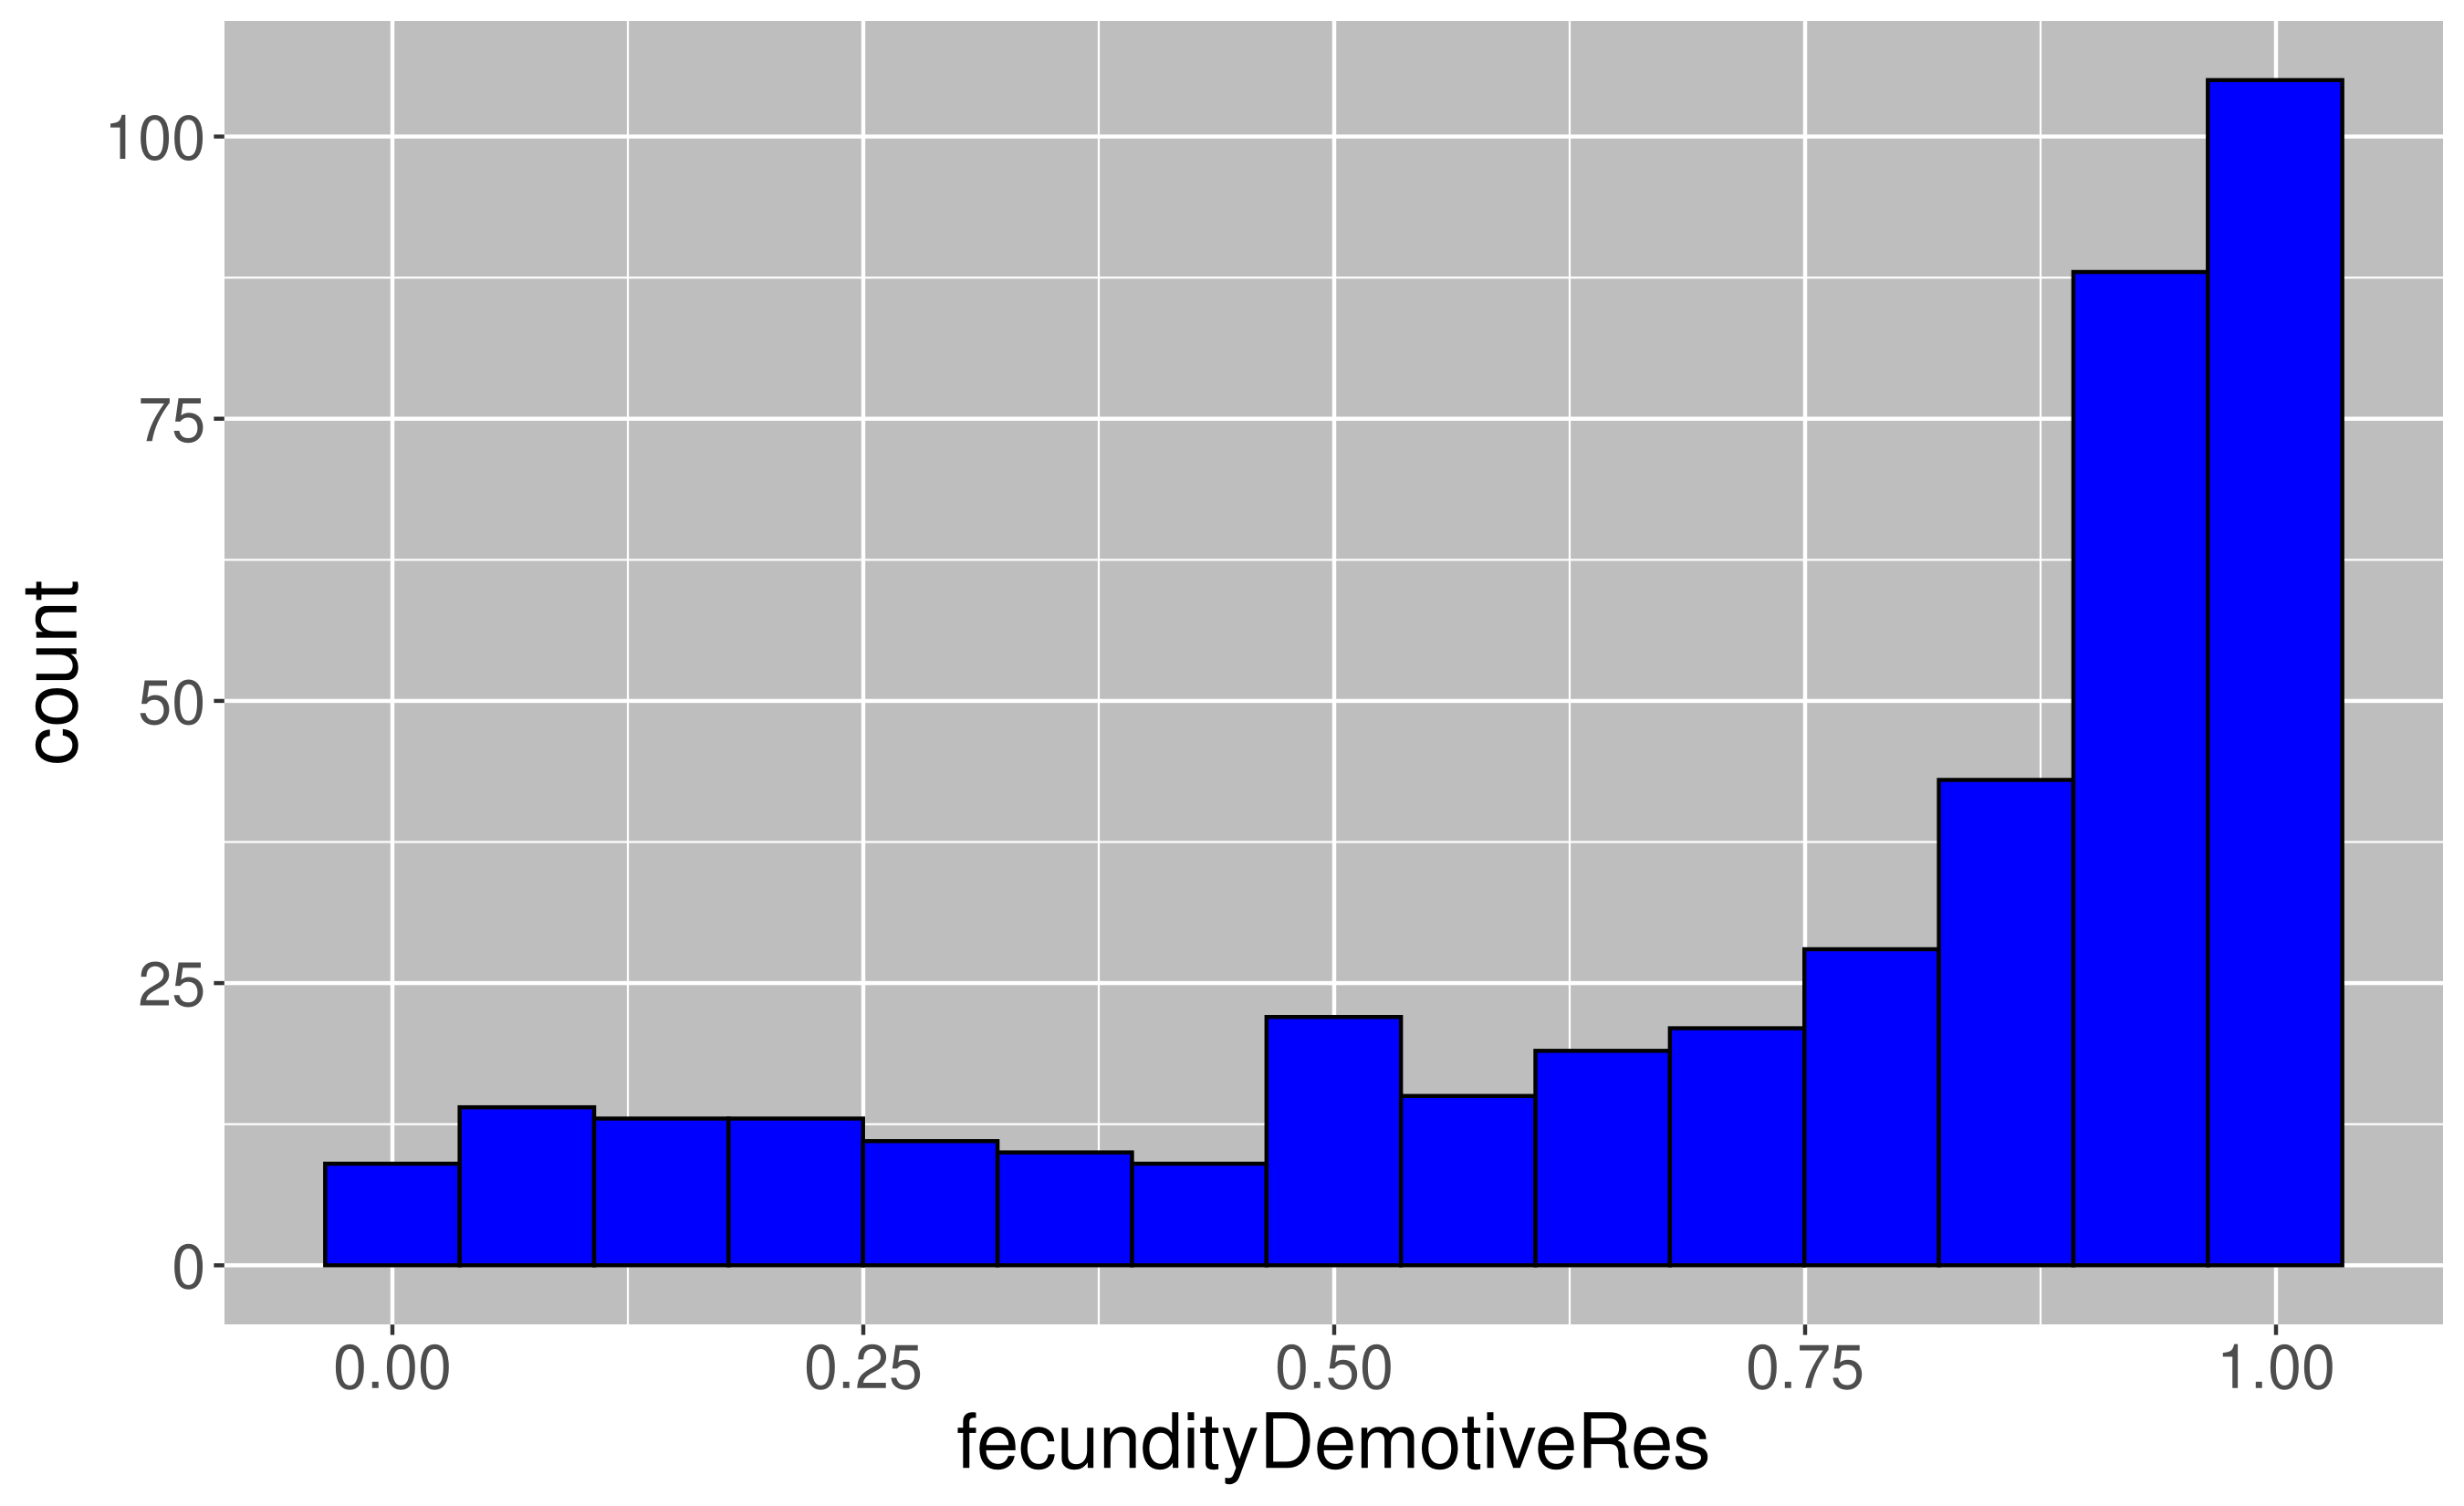
\includegraphics[width=5in]{/home/akara/workspace/R/CHAAHK/REPLACEME/figures/5-22}
	Plot corresponding to Figure 5.22 of Kara 2018
	\label{fig:5-22}
\end{figure}
\begin{figure}[H]
	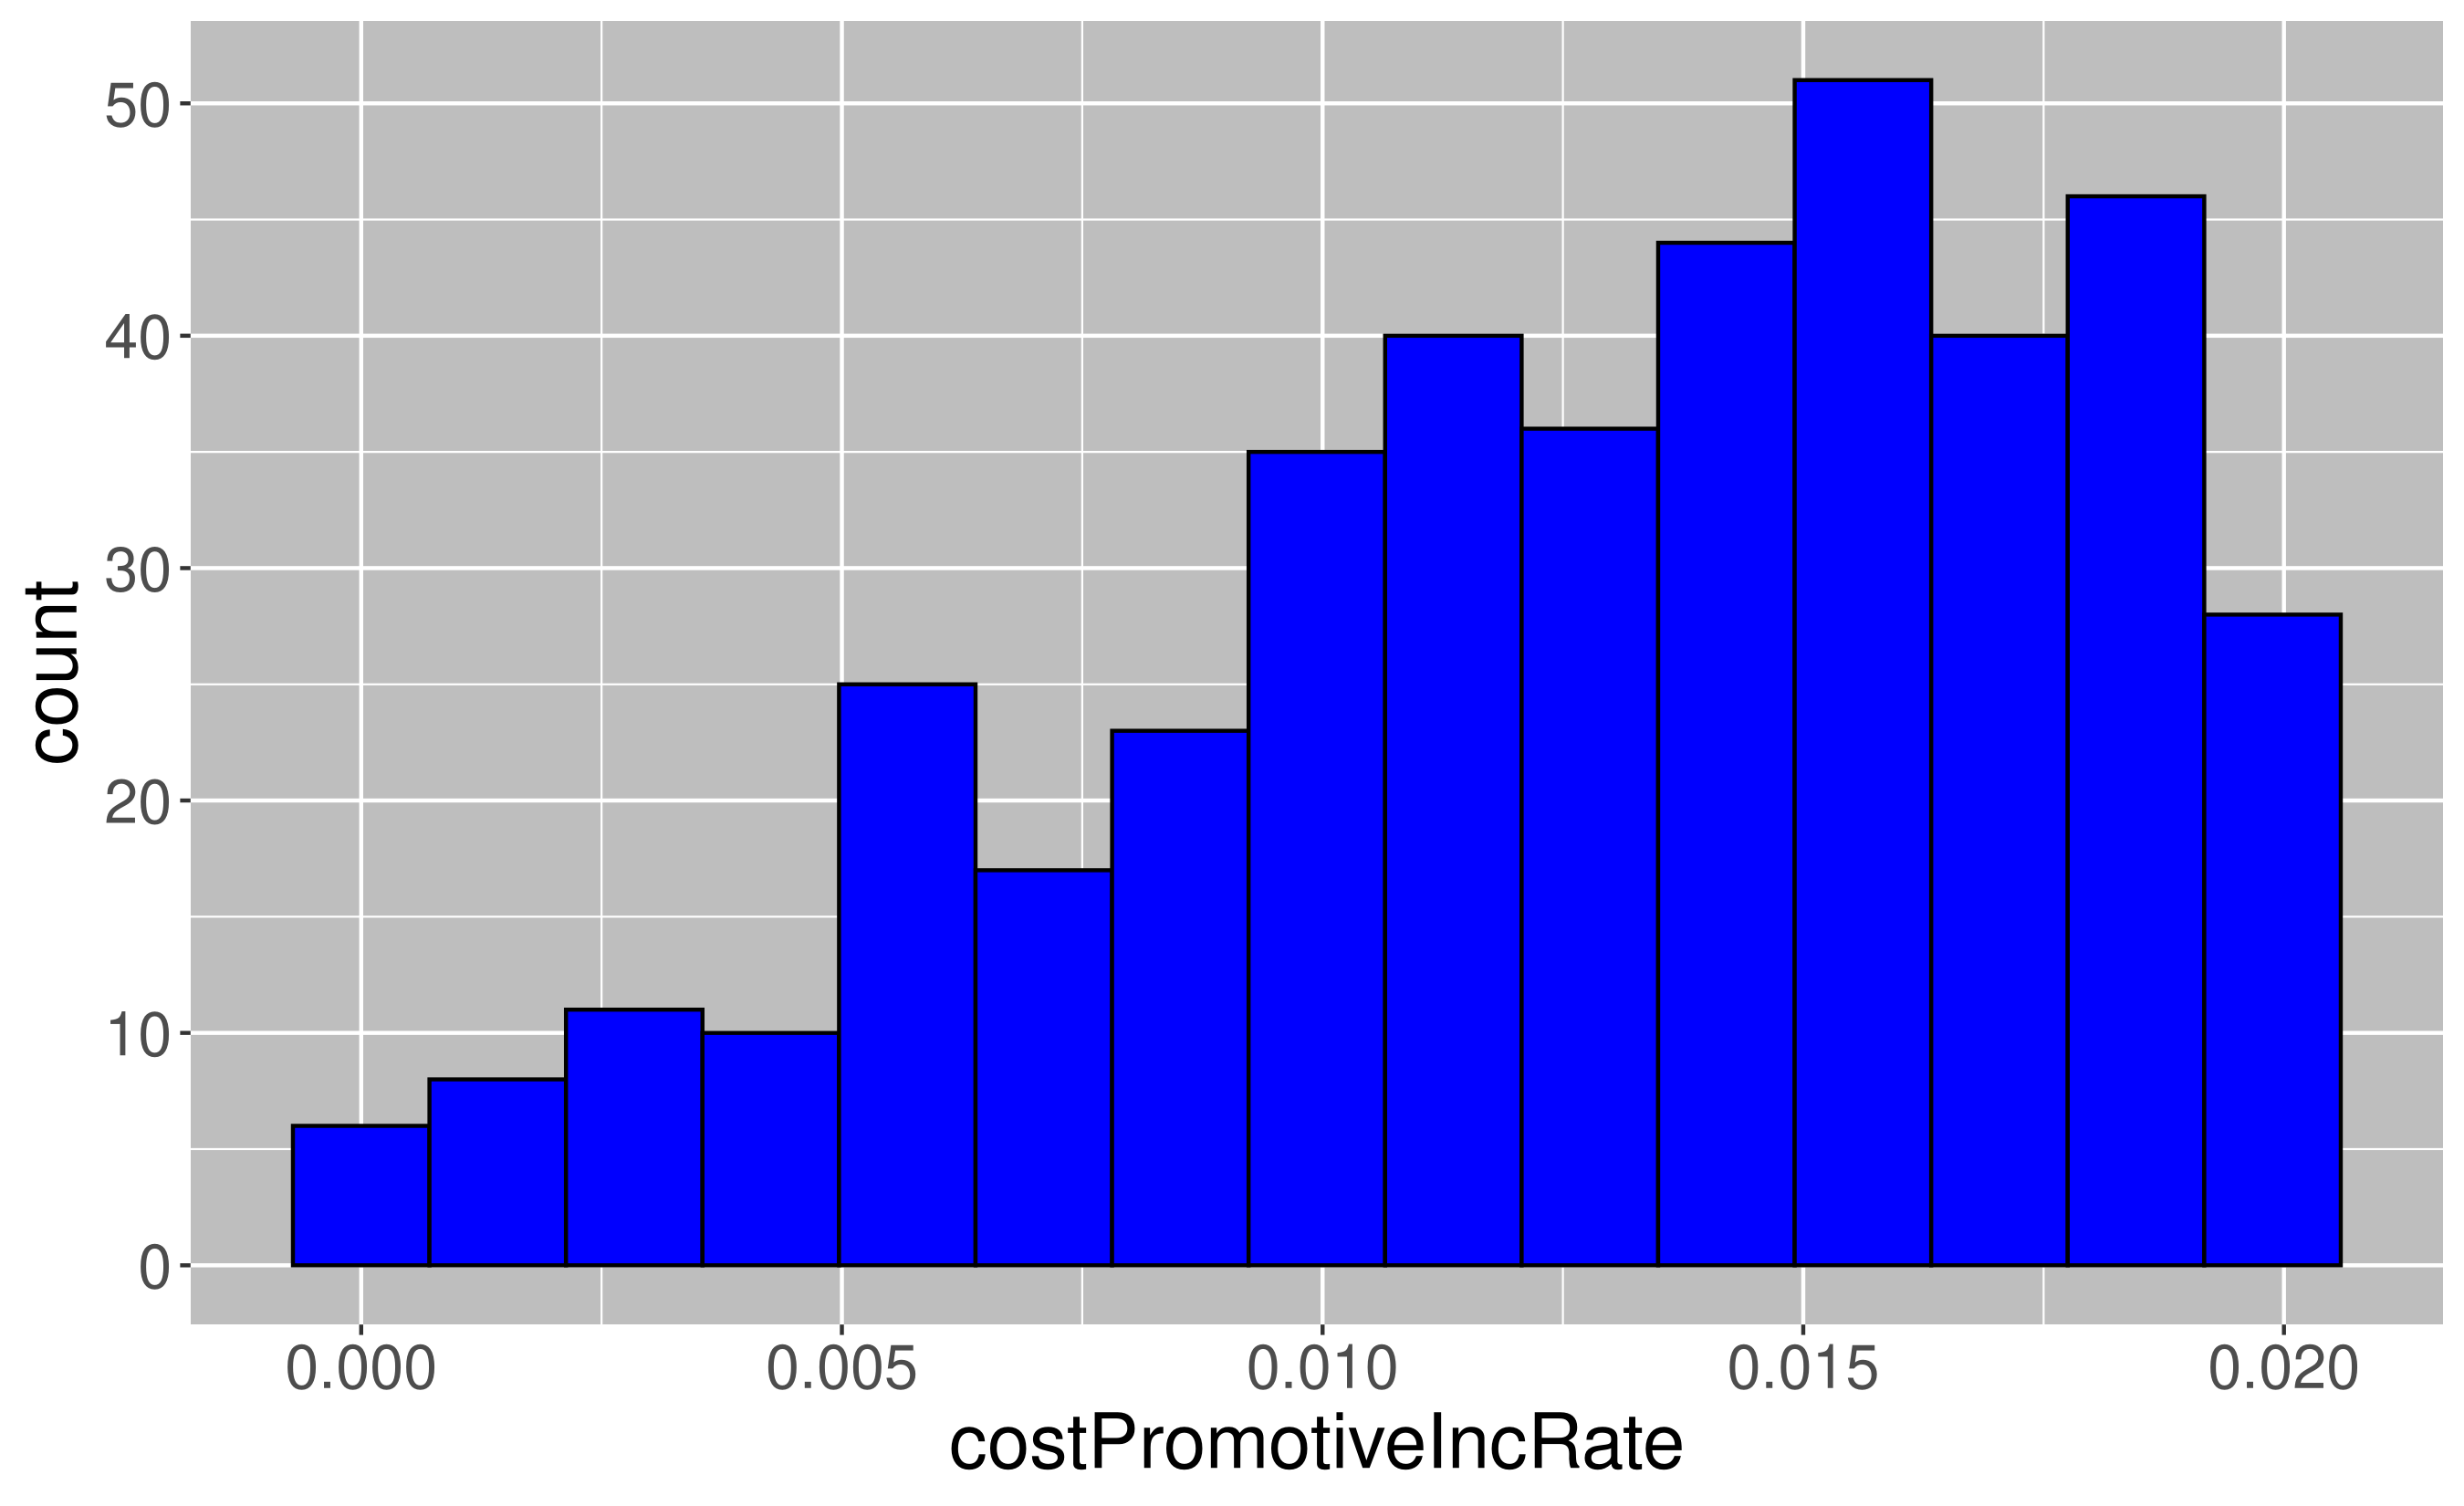
\includegraphics[width=5in]{/home/akara/workspace/R/CHAAHK/REPLACEME/figures/5-23}
	Plot corresponding to Figure 5.23 of Kara 2018
	\label{fig:5-23}
\end{figure}
\begin{figure}[H]
	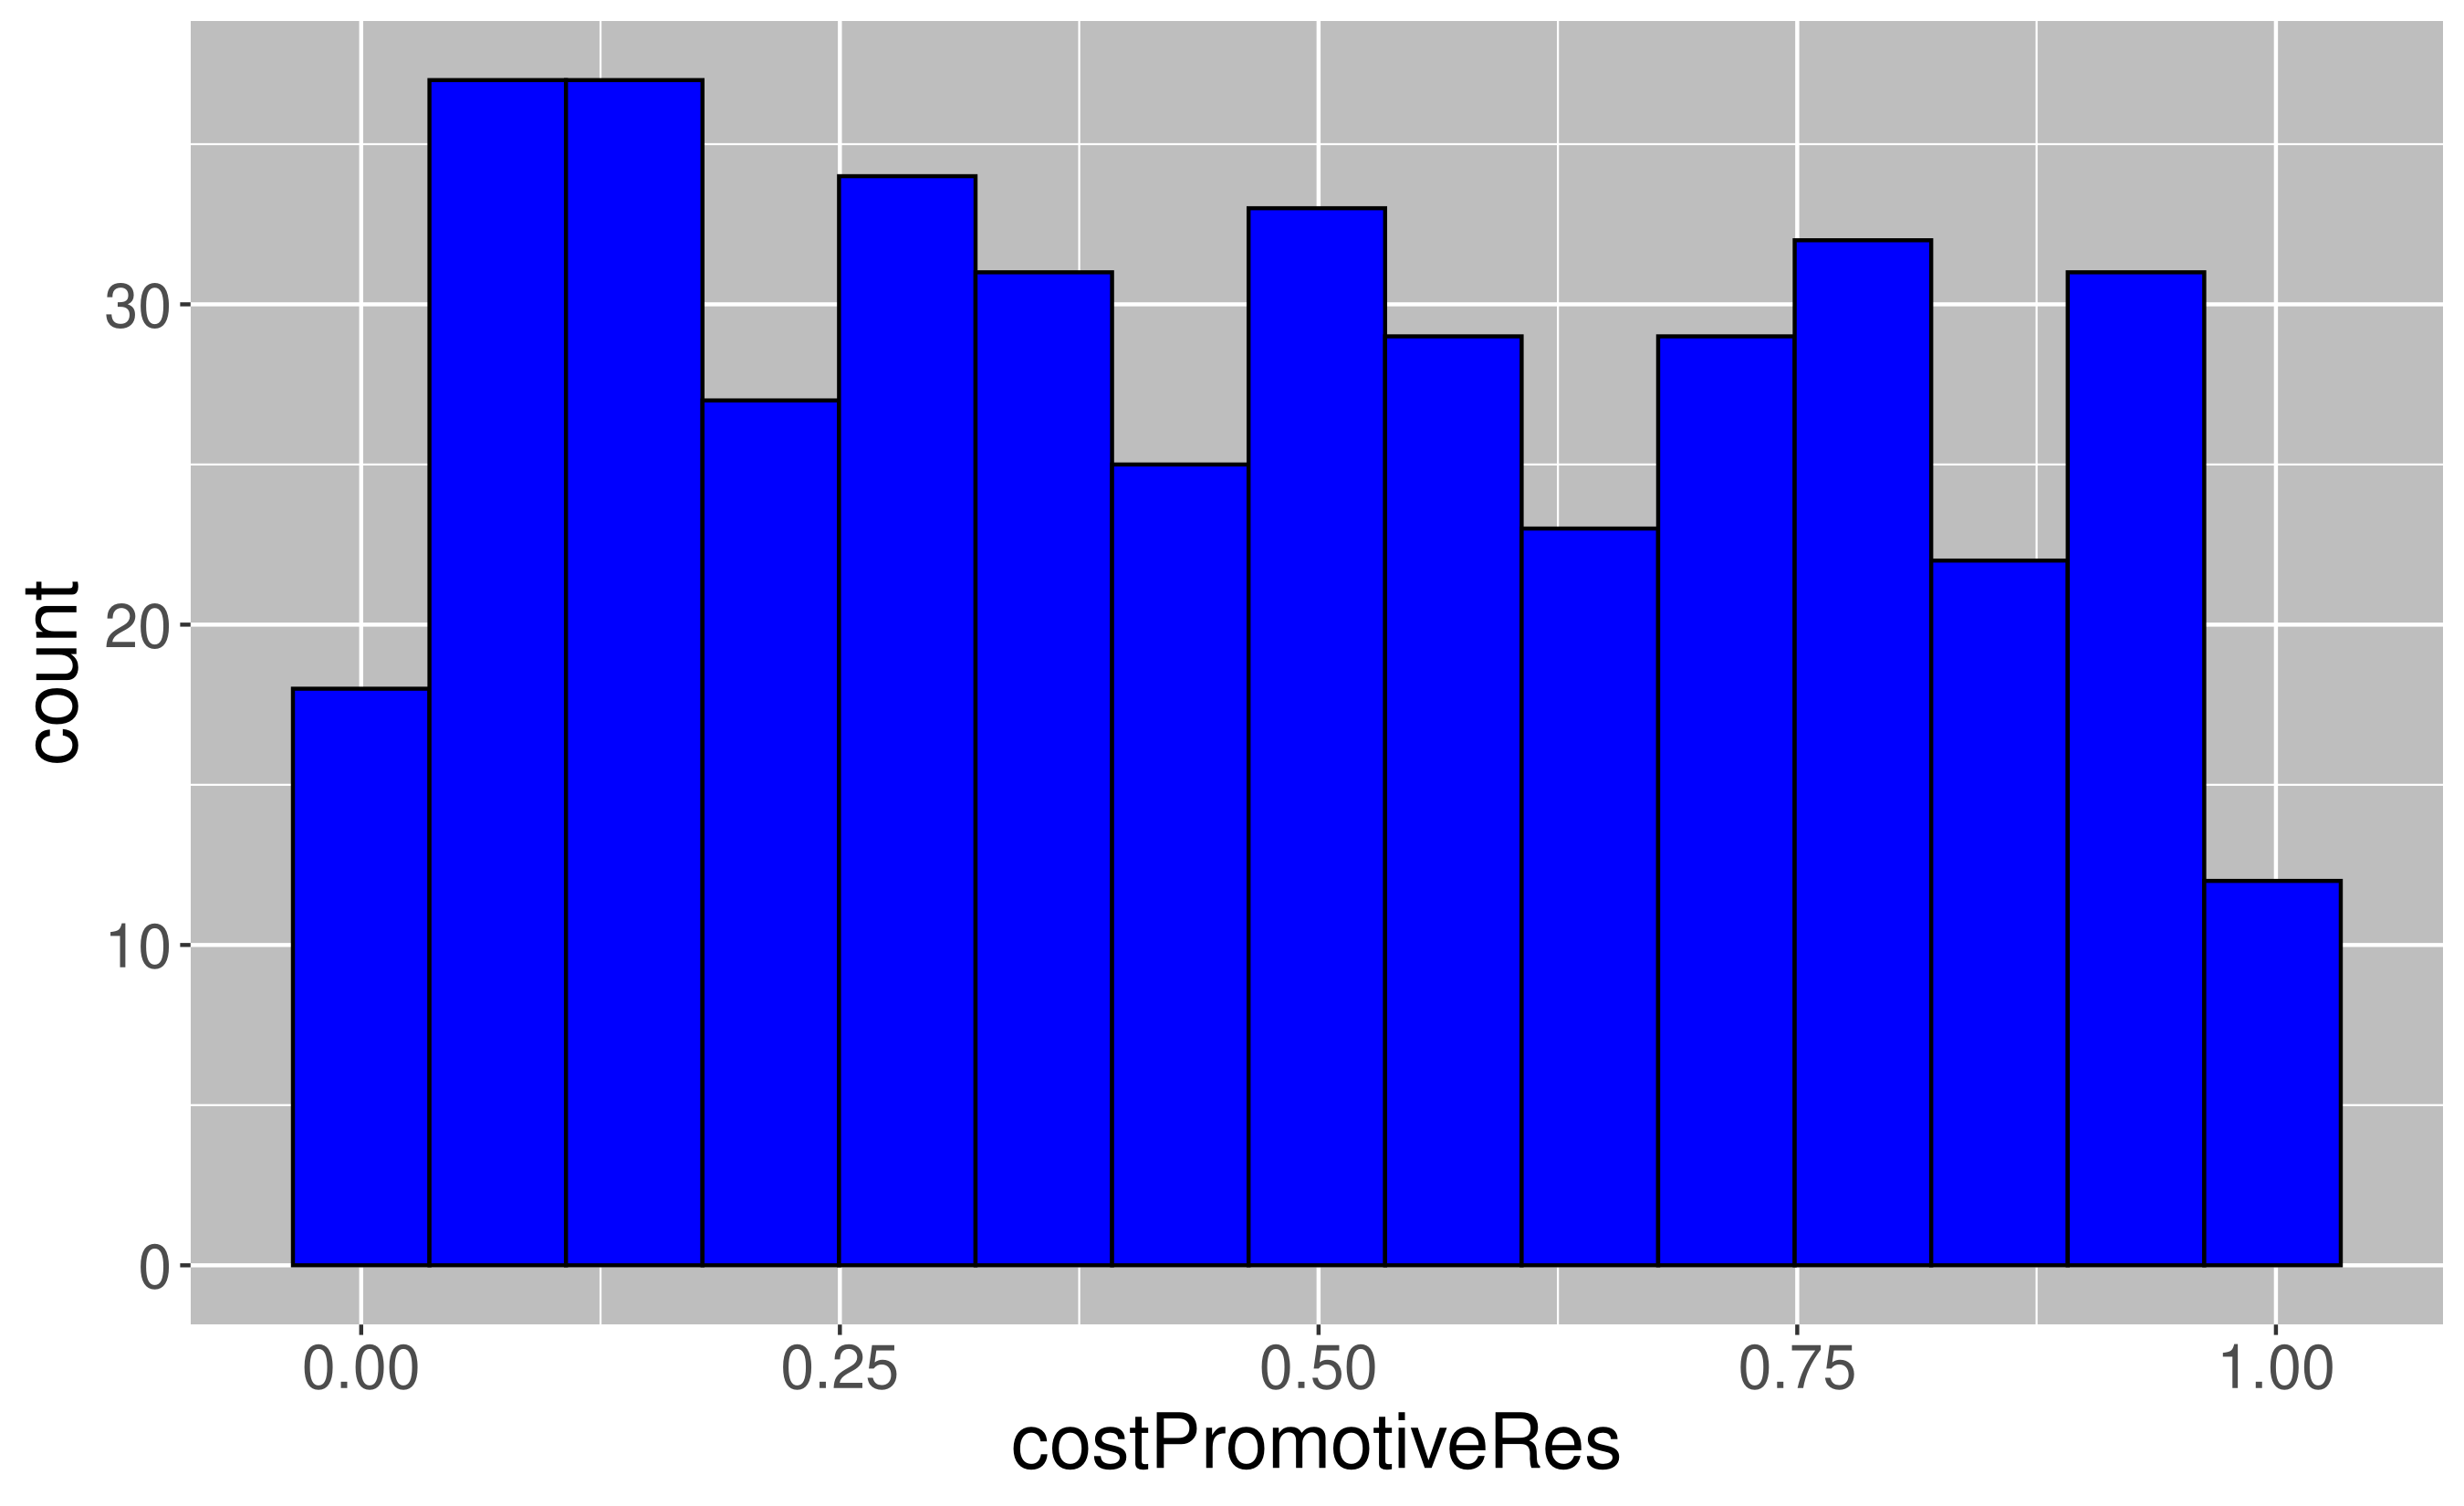
\includegraphics[width=5in]{/home/akara/workspace/R/CHAAHK/REPLACEME/figures/5-24}
	Plot corresponding to Figure 5.24 of Kara 2018
	\label{fig:5-24}
\end{figure}
\begin{figure}[H]
	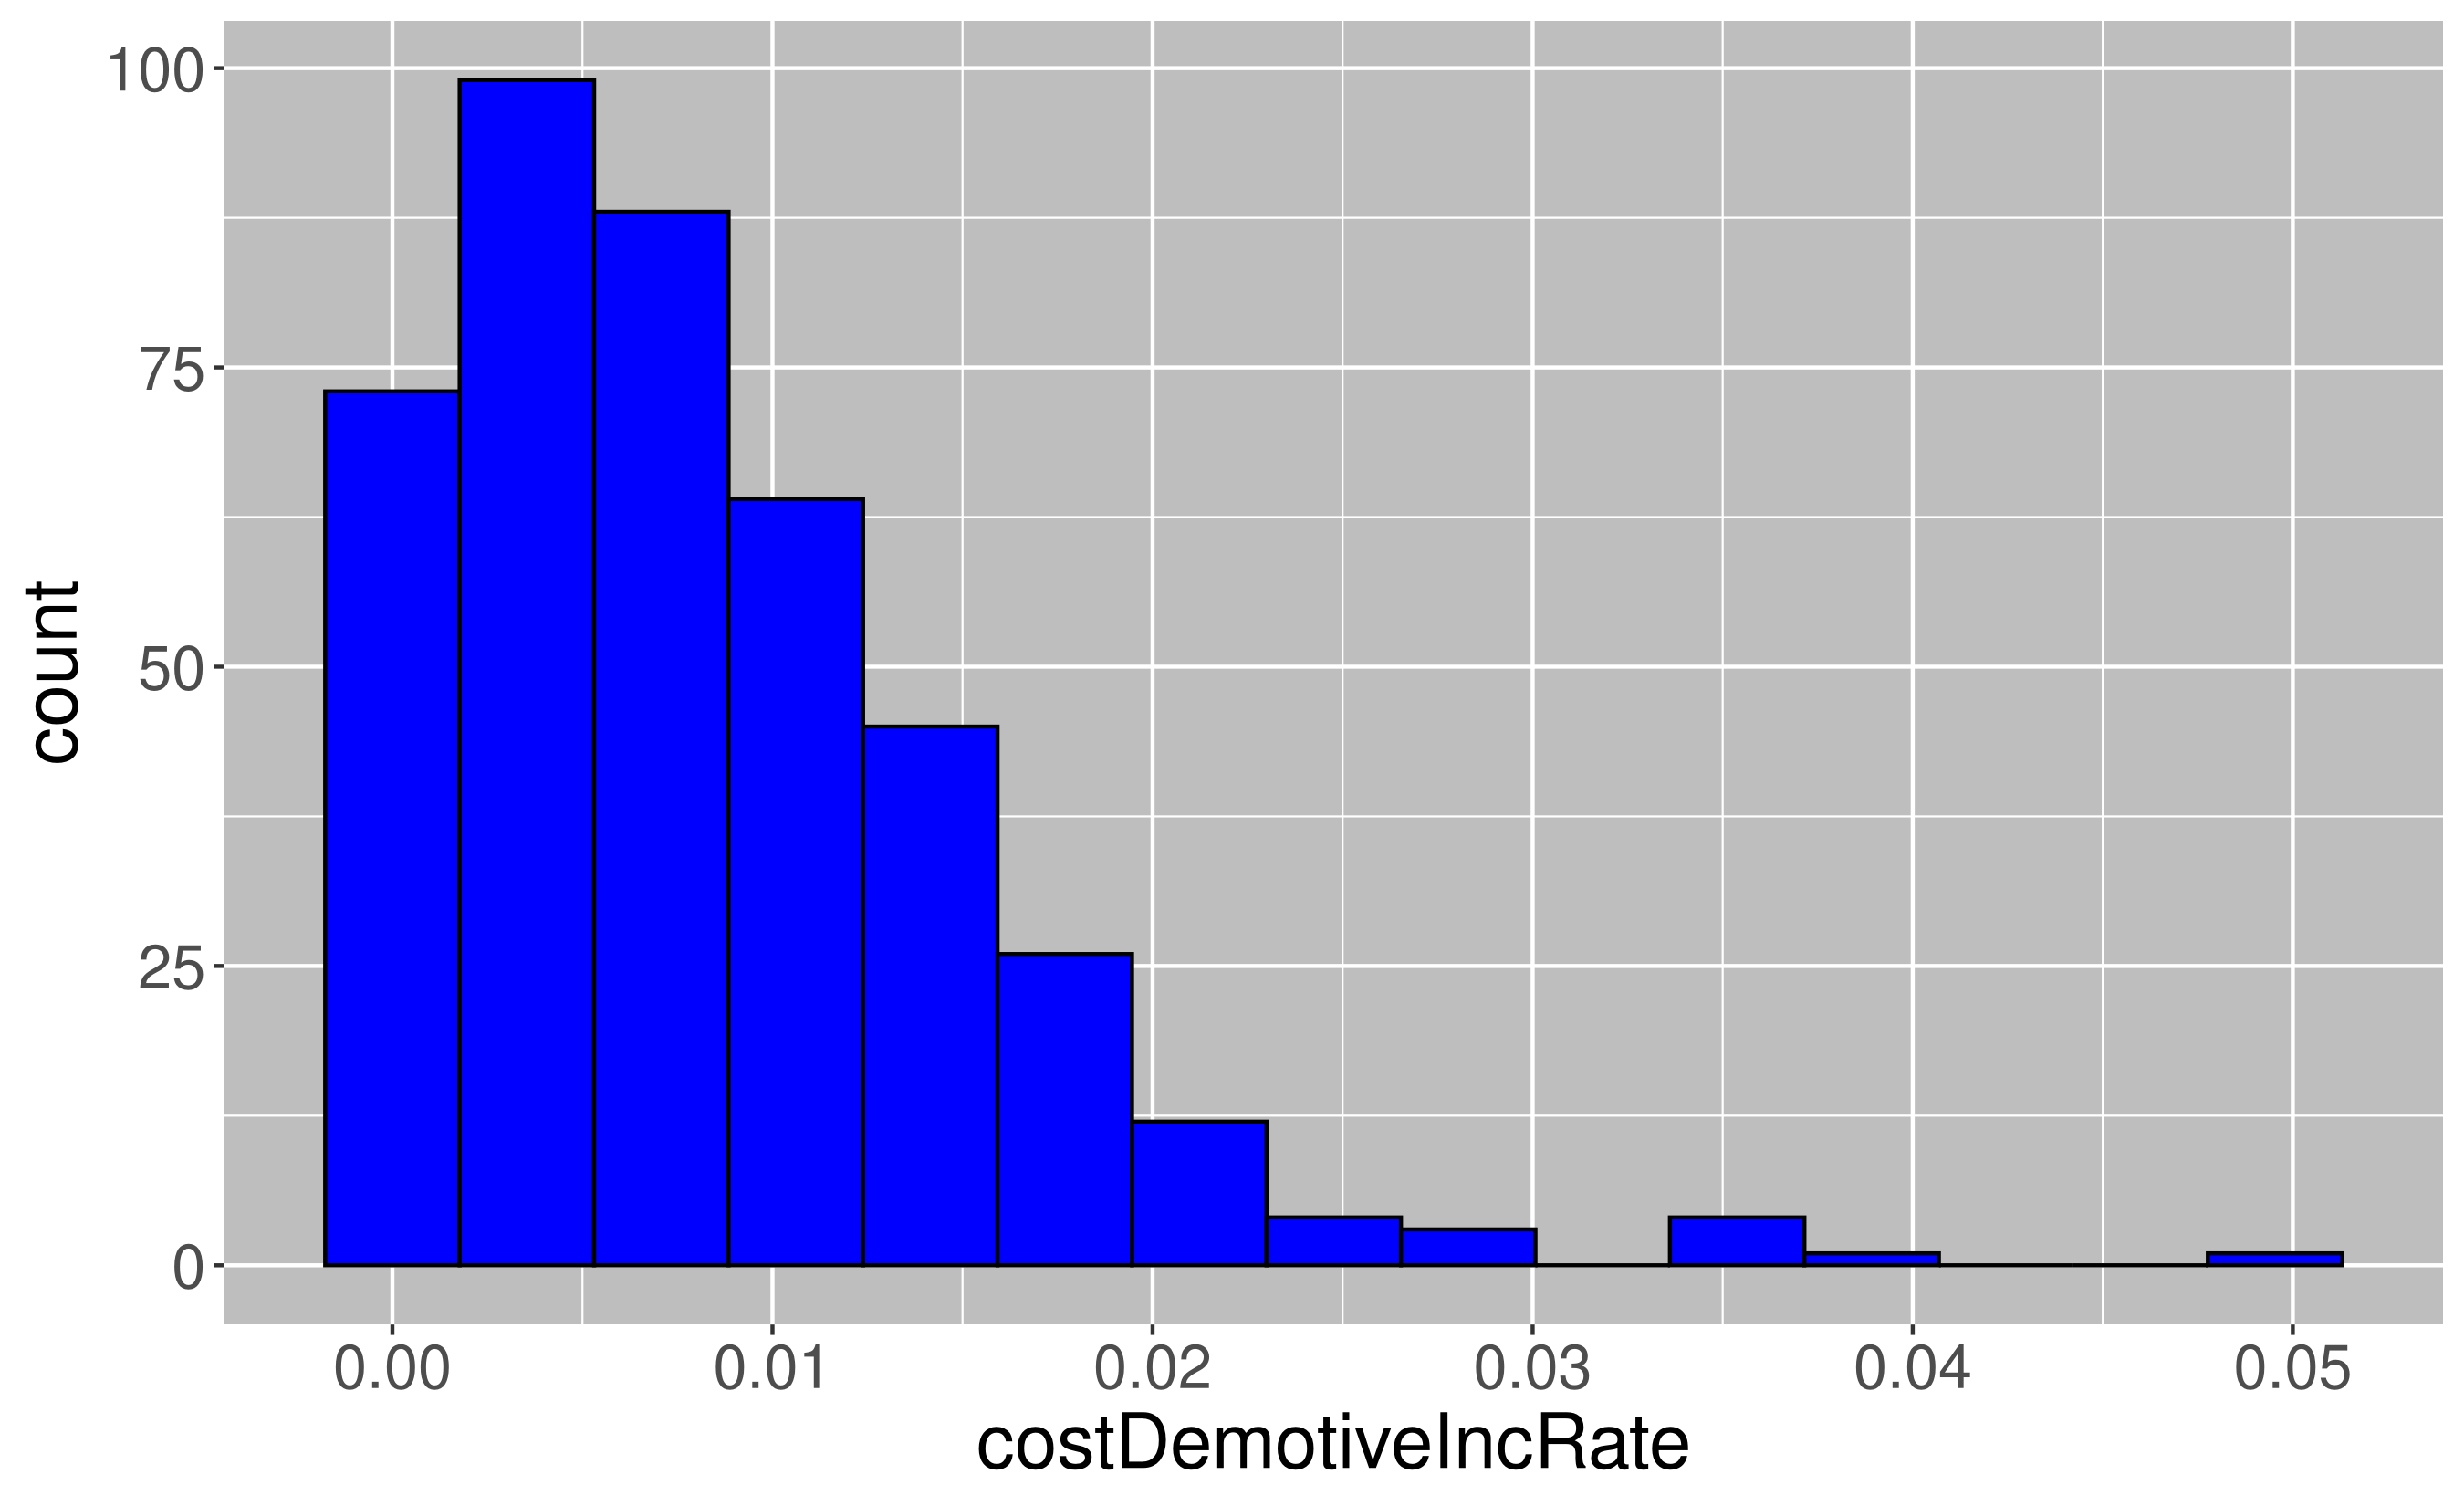
\includegraphics[width=5in]{/home/akara/workspace/R/CHAAHK/REPLACEME/figures/5-25}
	Plot corresponding to Figure 5.25 of Kara 2018
	\label{fig:5-25}
\end{figure}
\begin{figure}[H]
	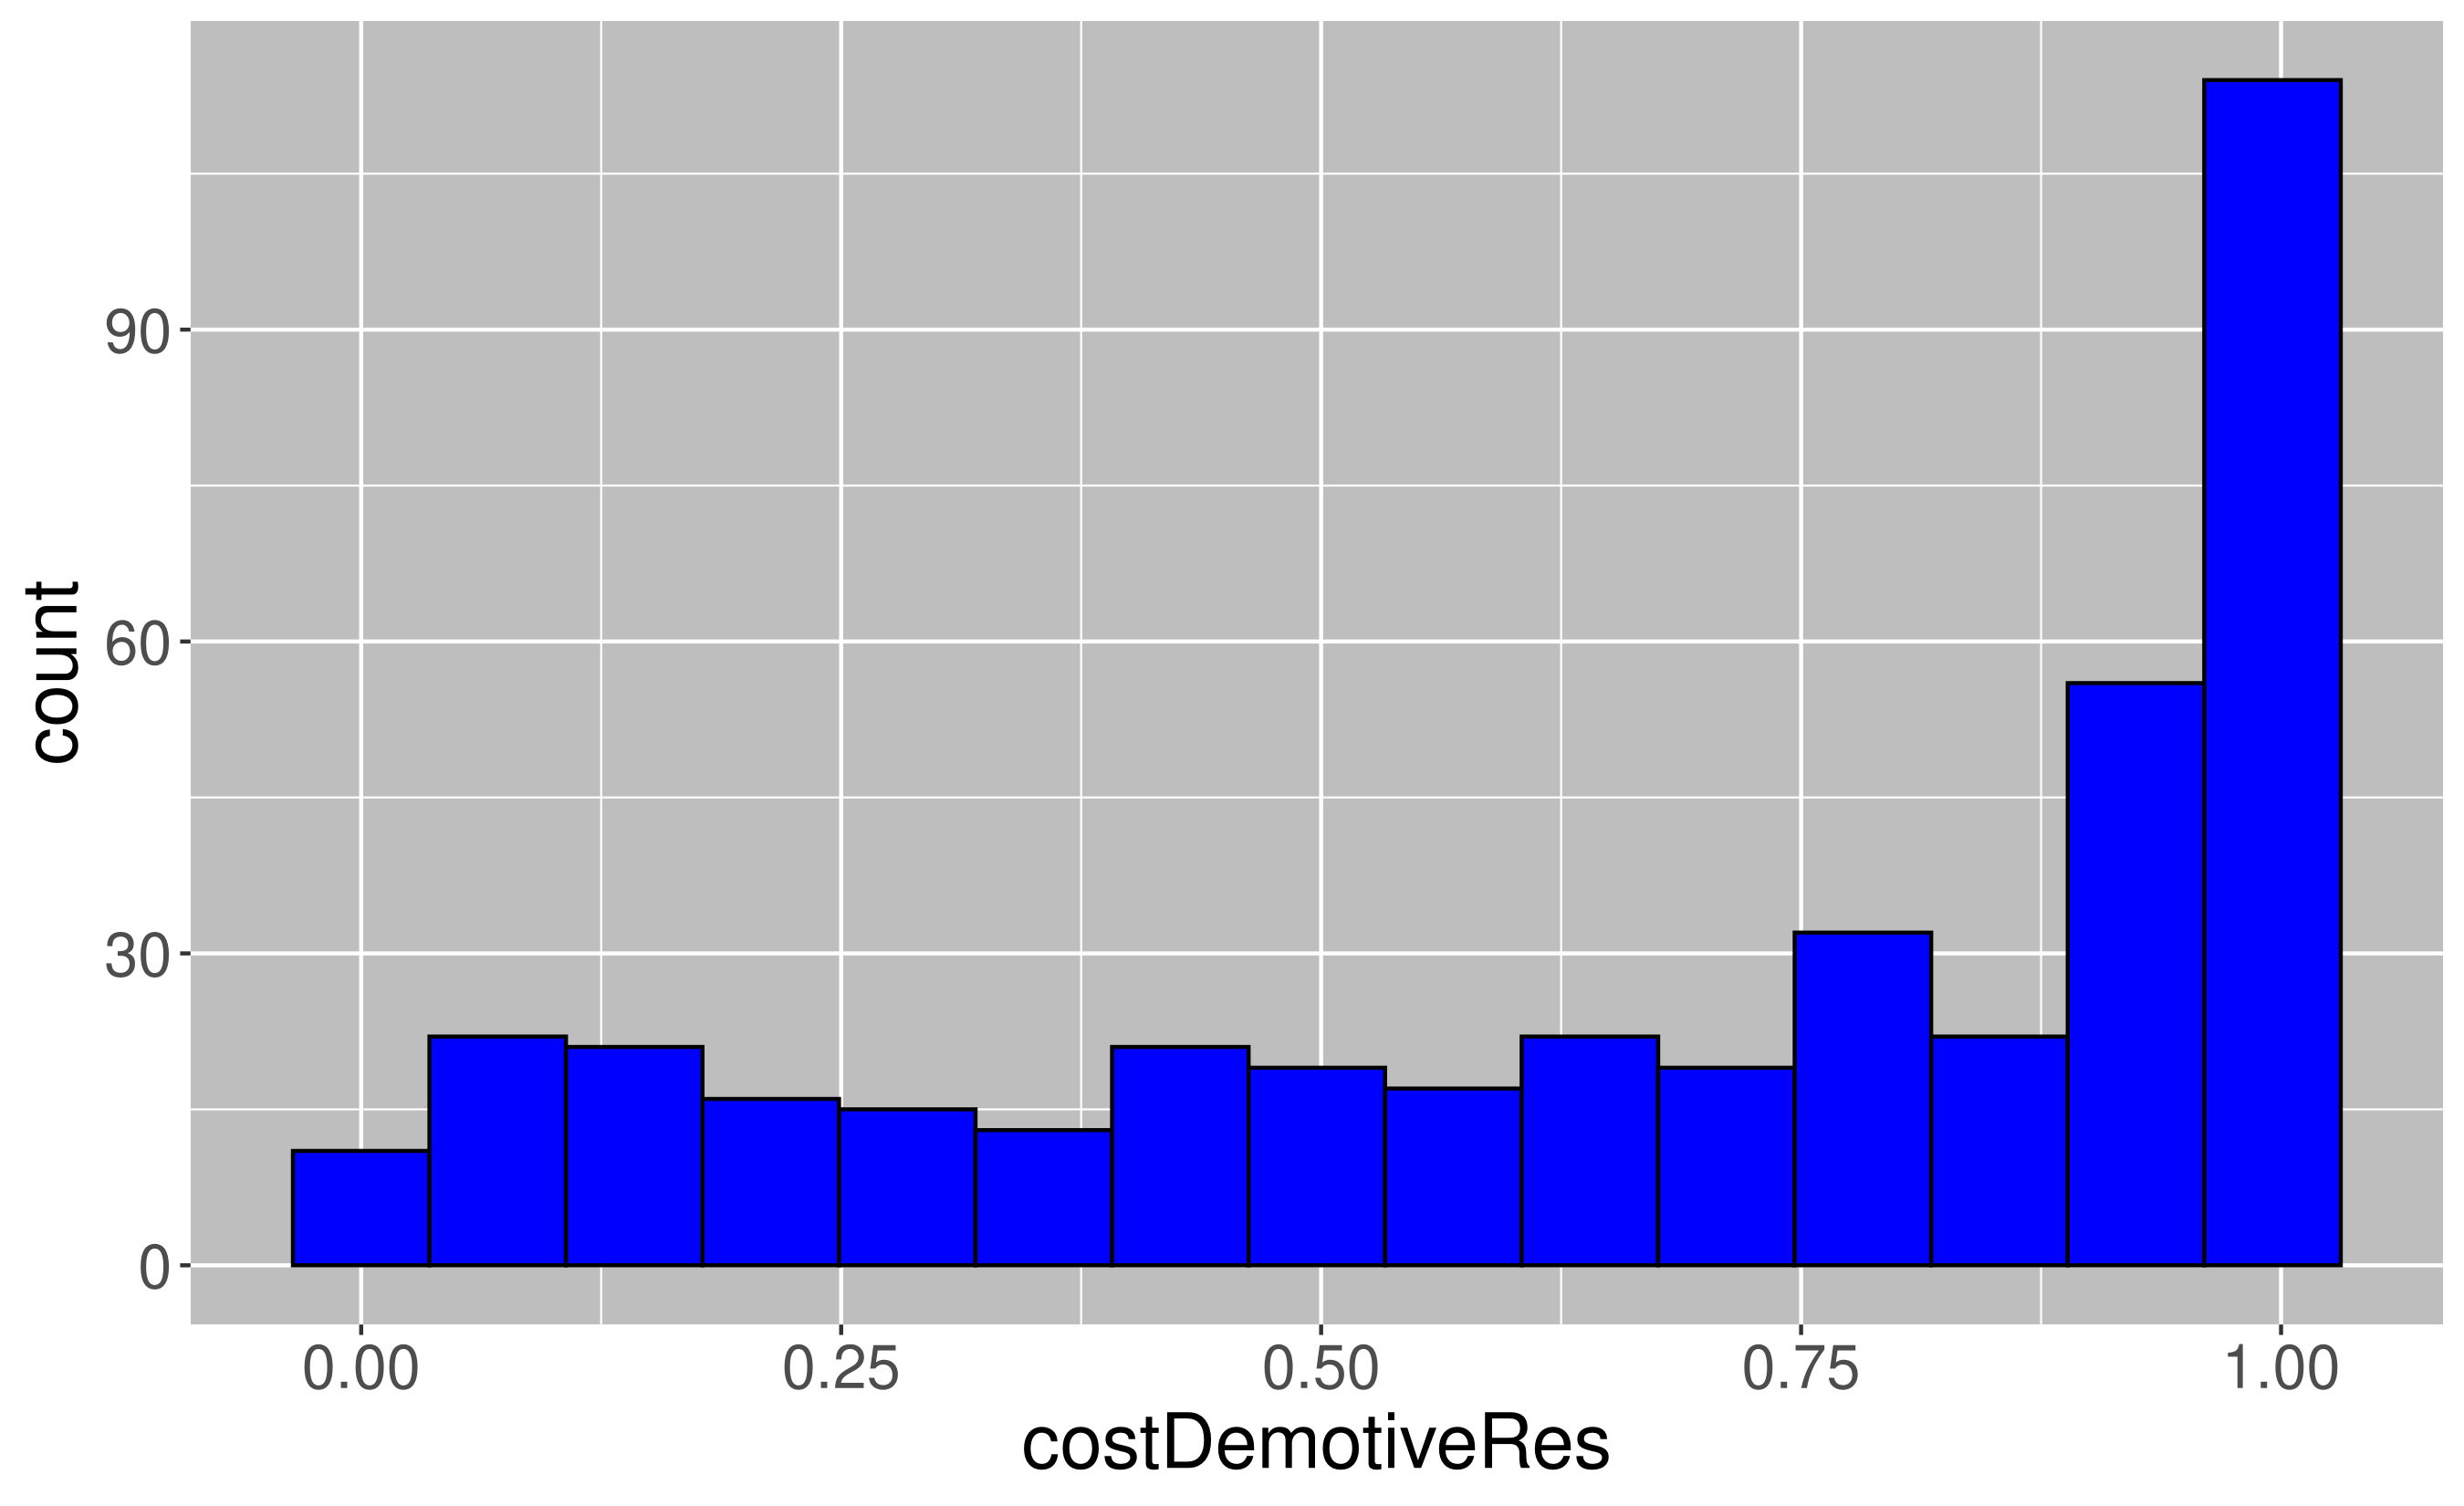
\includegraphics[width=5in]{/home/akara/workspace/R/CHAAHK/REPLACEME/figures/5-26}
	Plot corresponding to Figure 5.26 of Kara 2018
	\label{fig:5-26}
\end{figure}
\begin{figure}[H]
	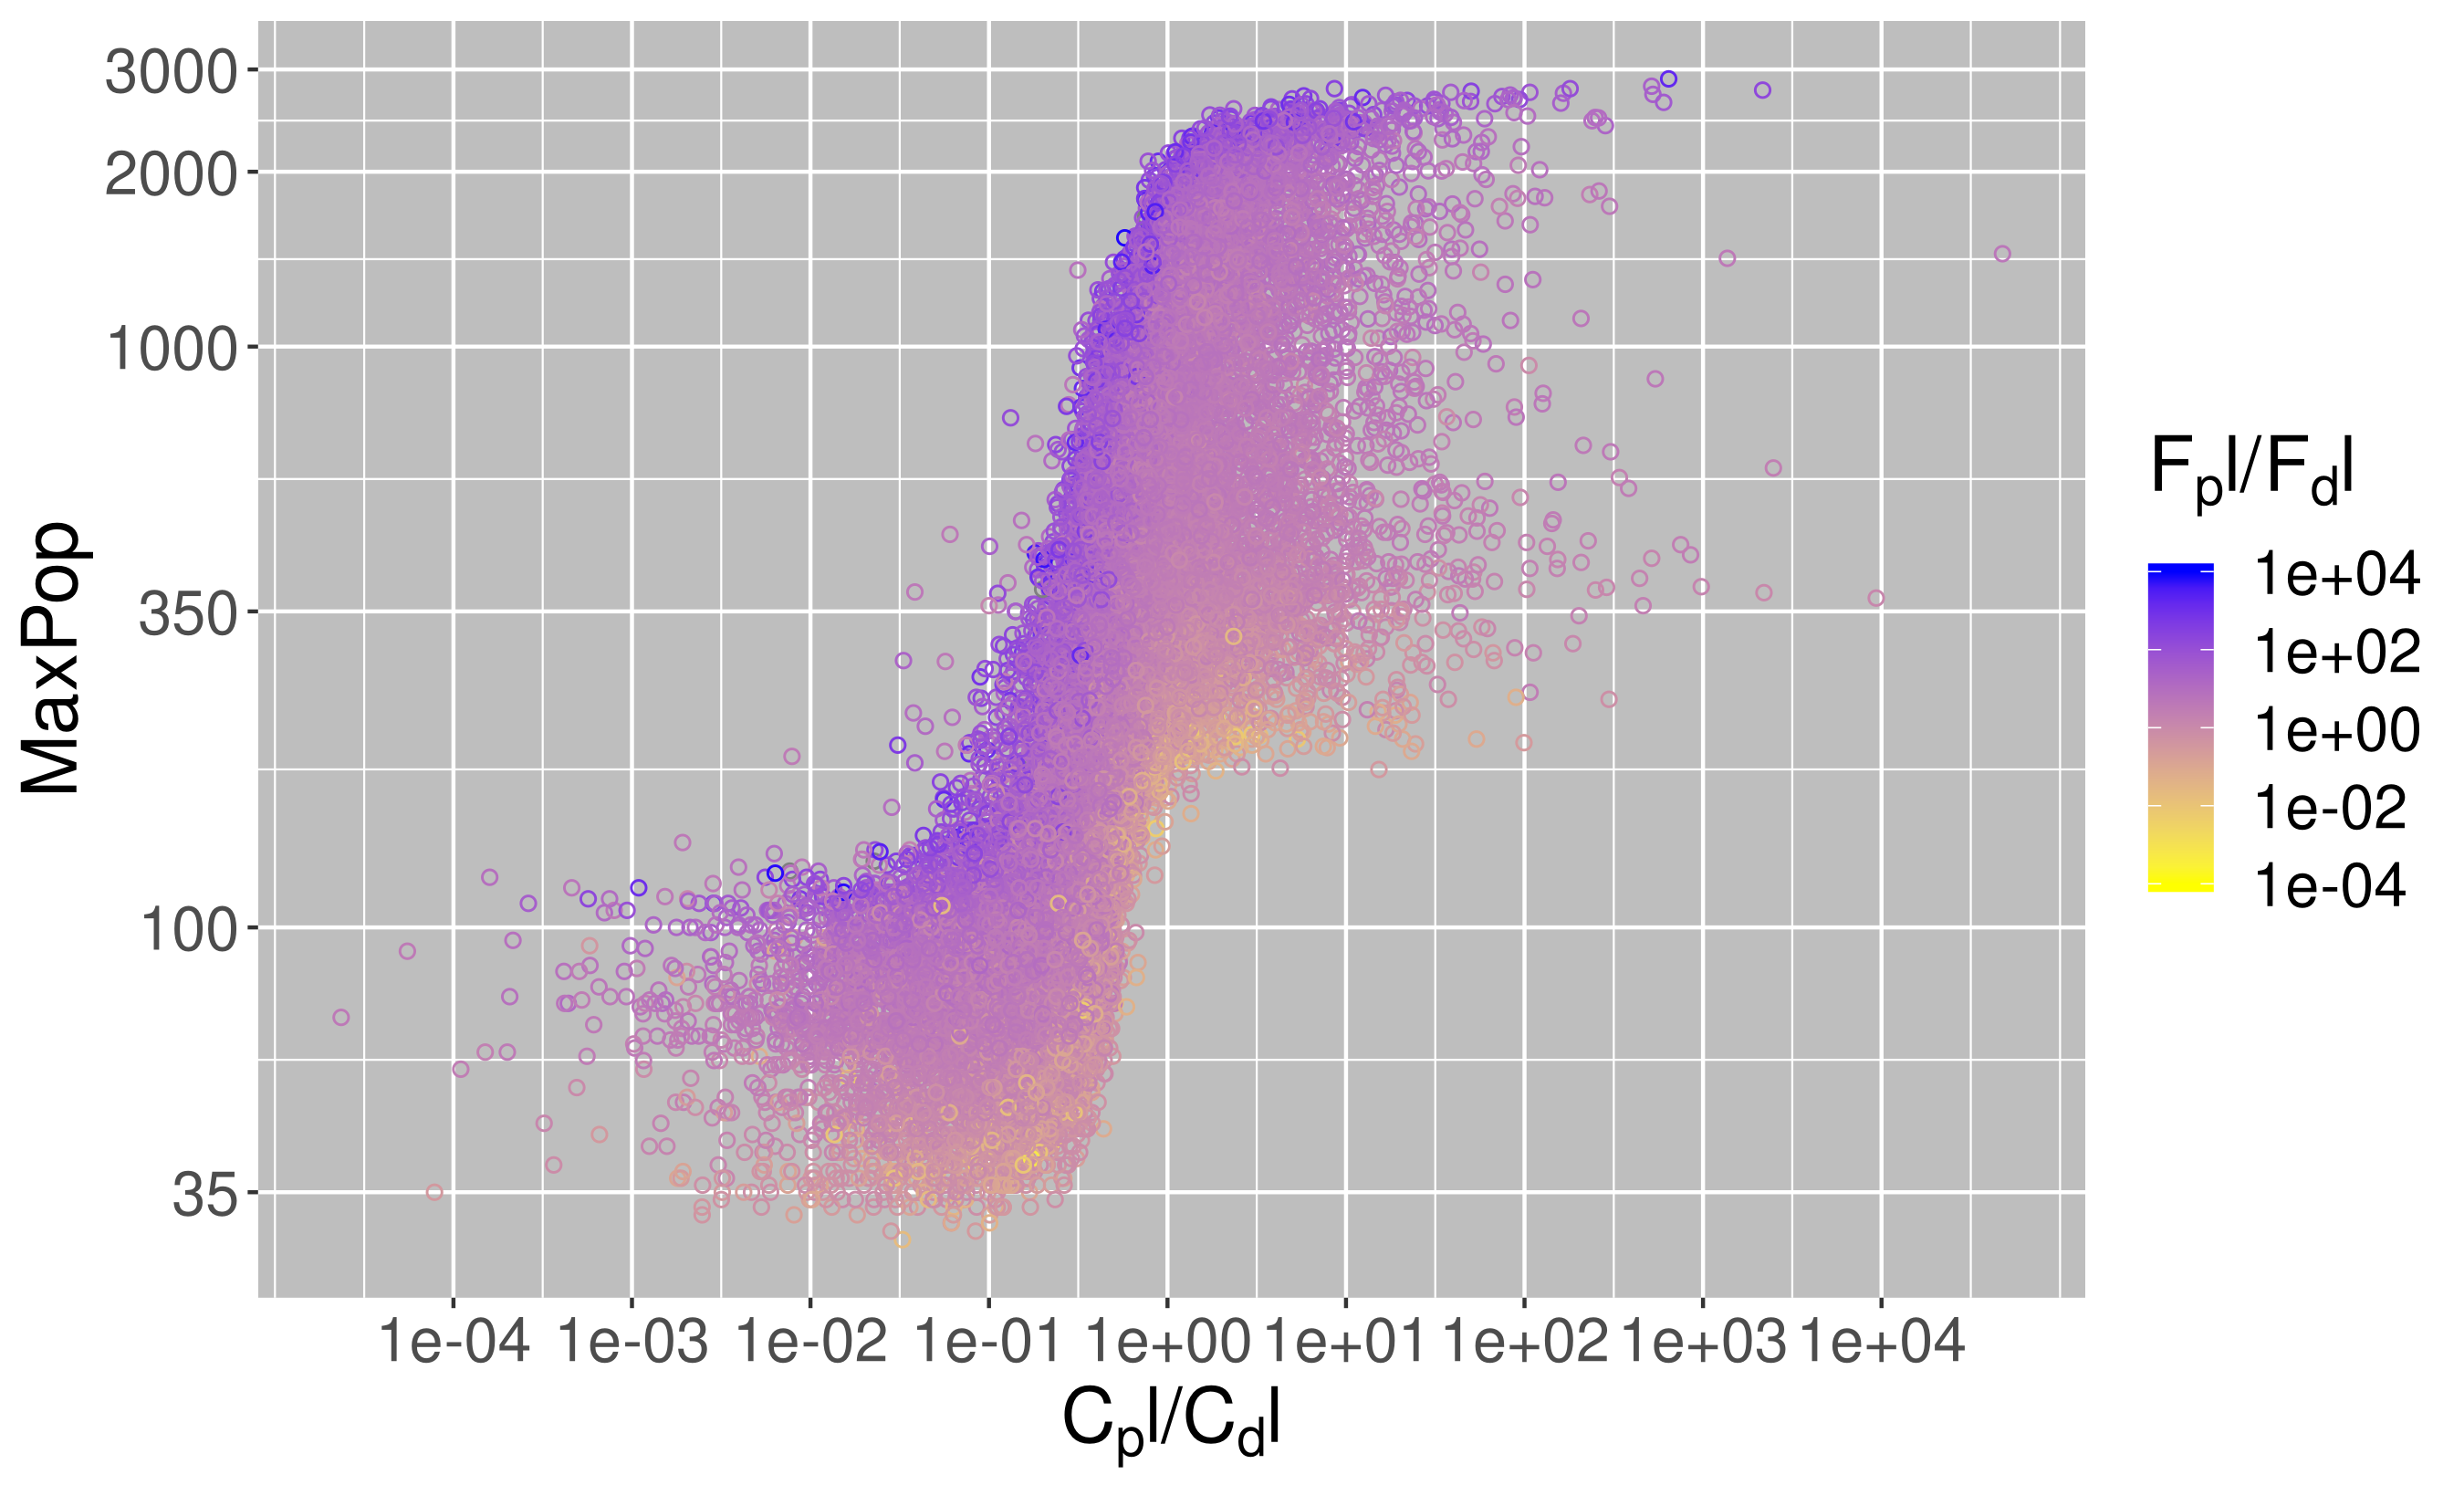
\includegraphics[width=5in]{/home/akara/workspace/R/CHAAHK/REPLACEME/figures/5-27}
	Plot corresponding to Figure 5.27 of Kara 2018
	\label{fig:5-27}
\end{figure}
\begin{figure}[H]
	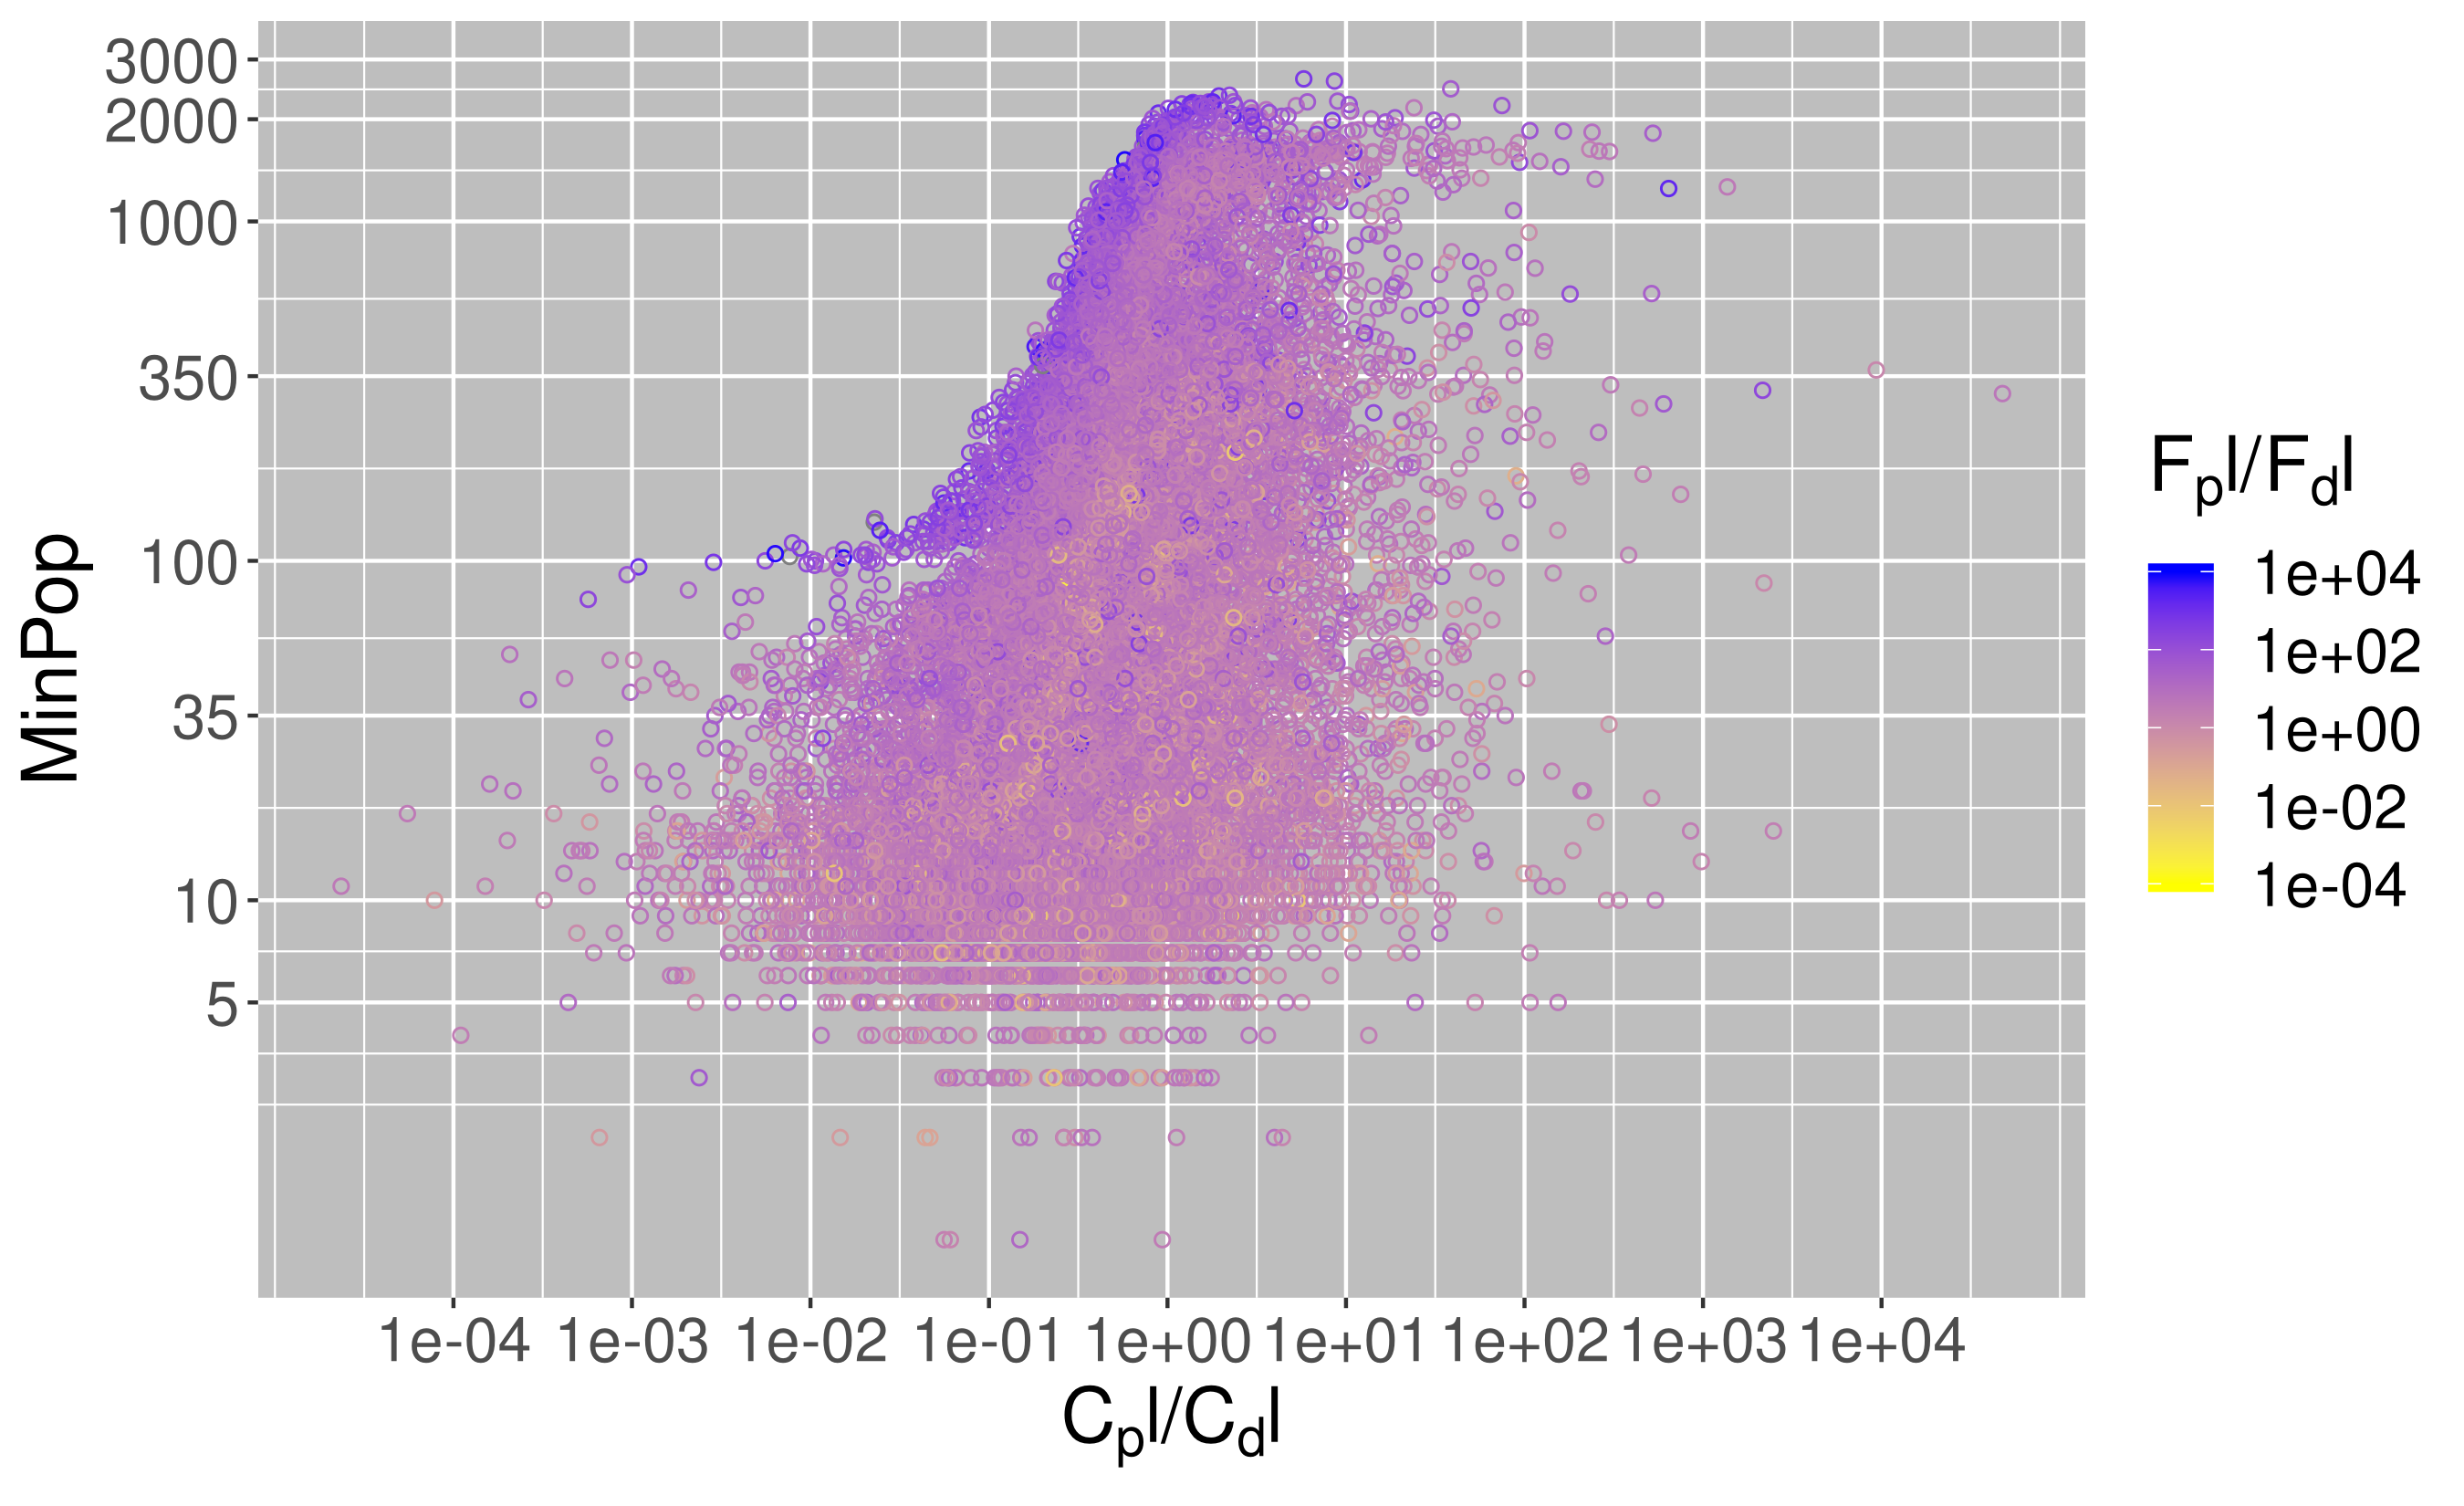
\includegraphics[width=5in]{/home/akara/workspace/R/CHAAHK/REPLACEME/figures/5-28}
	Plot corresponding to Figure 5.28 of Kara 2018
	\label{fig:5-28}
\end{figure}
\begin{figure}[H]
	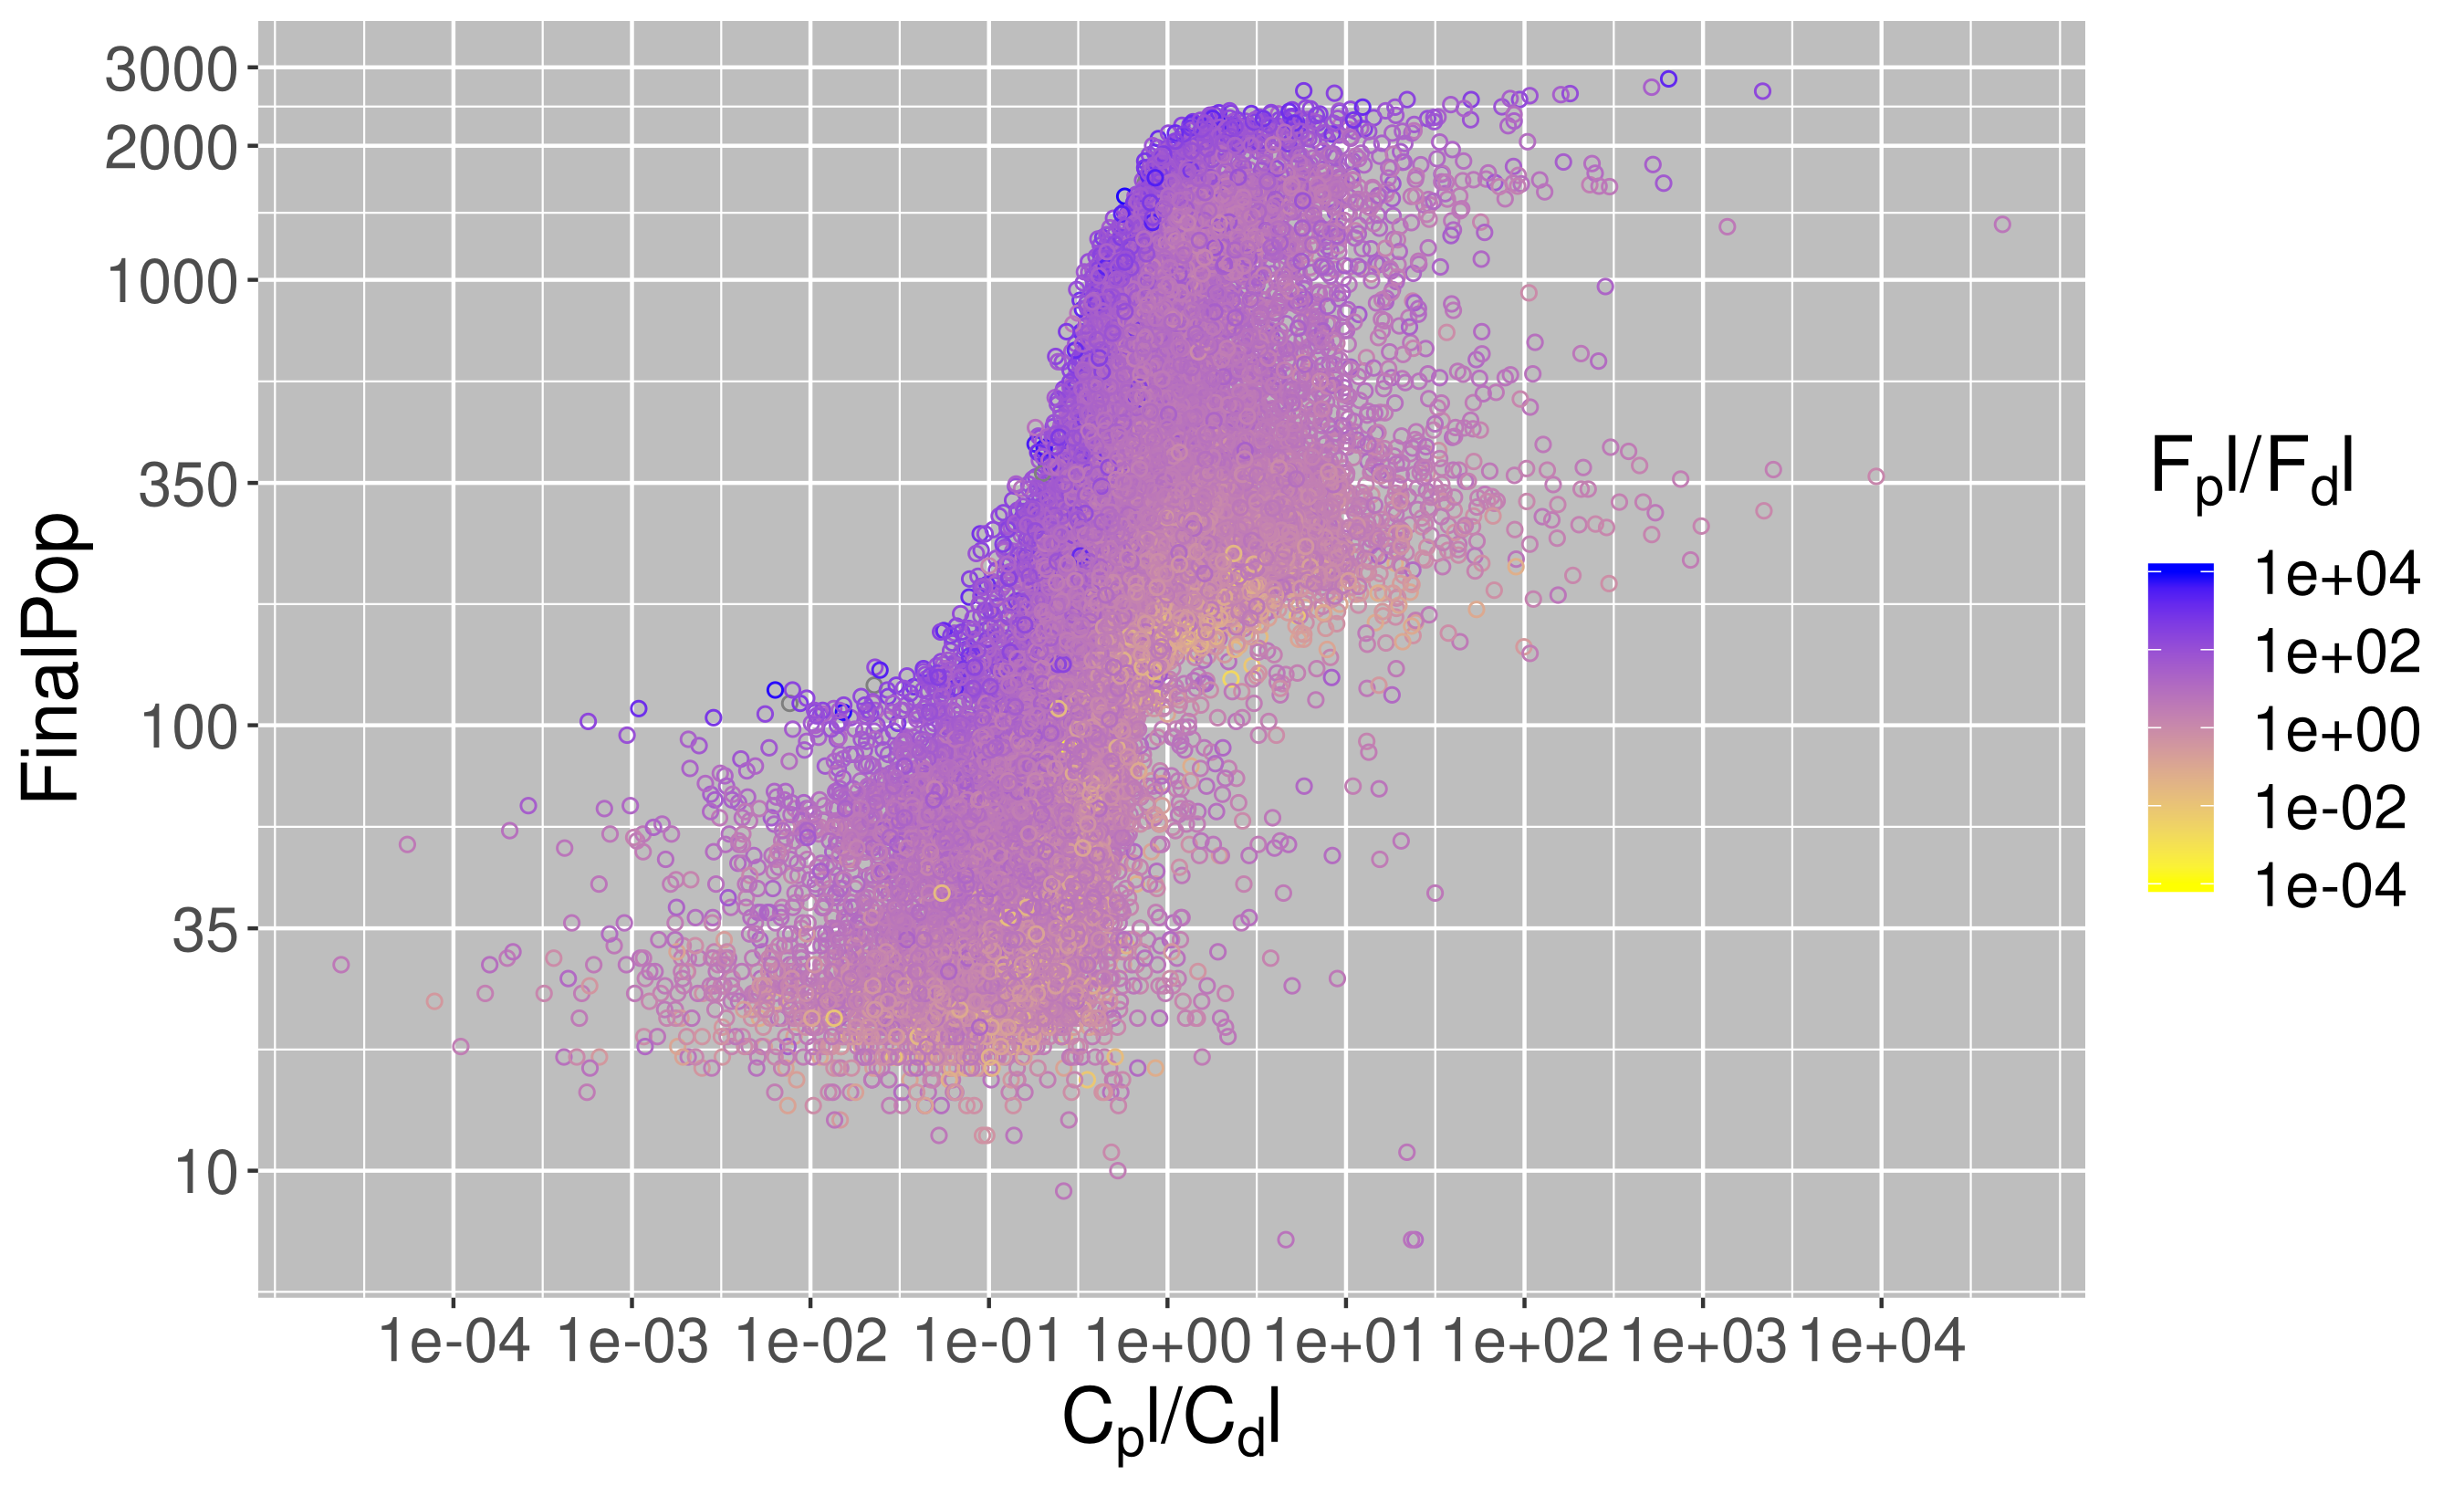
\includegraphics[width=5in]{/home/akara/workspace/R/CHAAHK/REPLACEME/figures/5-29}
	Plot corresponding to Figure 5.29 of Kara 2018
	\label{fig:5-29}
\end{figure}
\begin{figure}[H]
	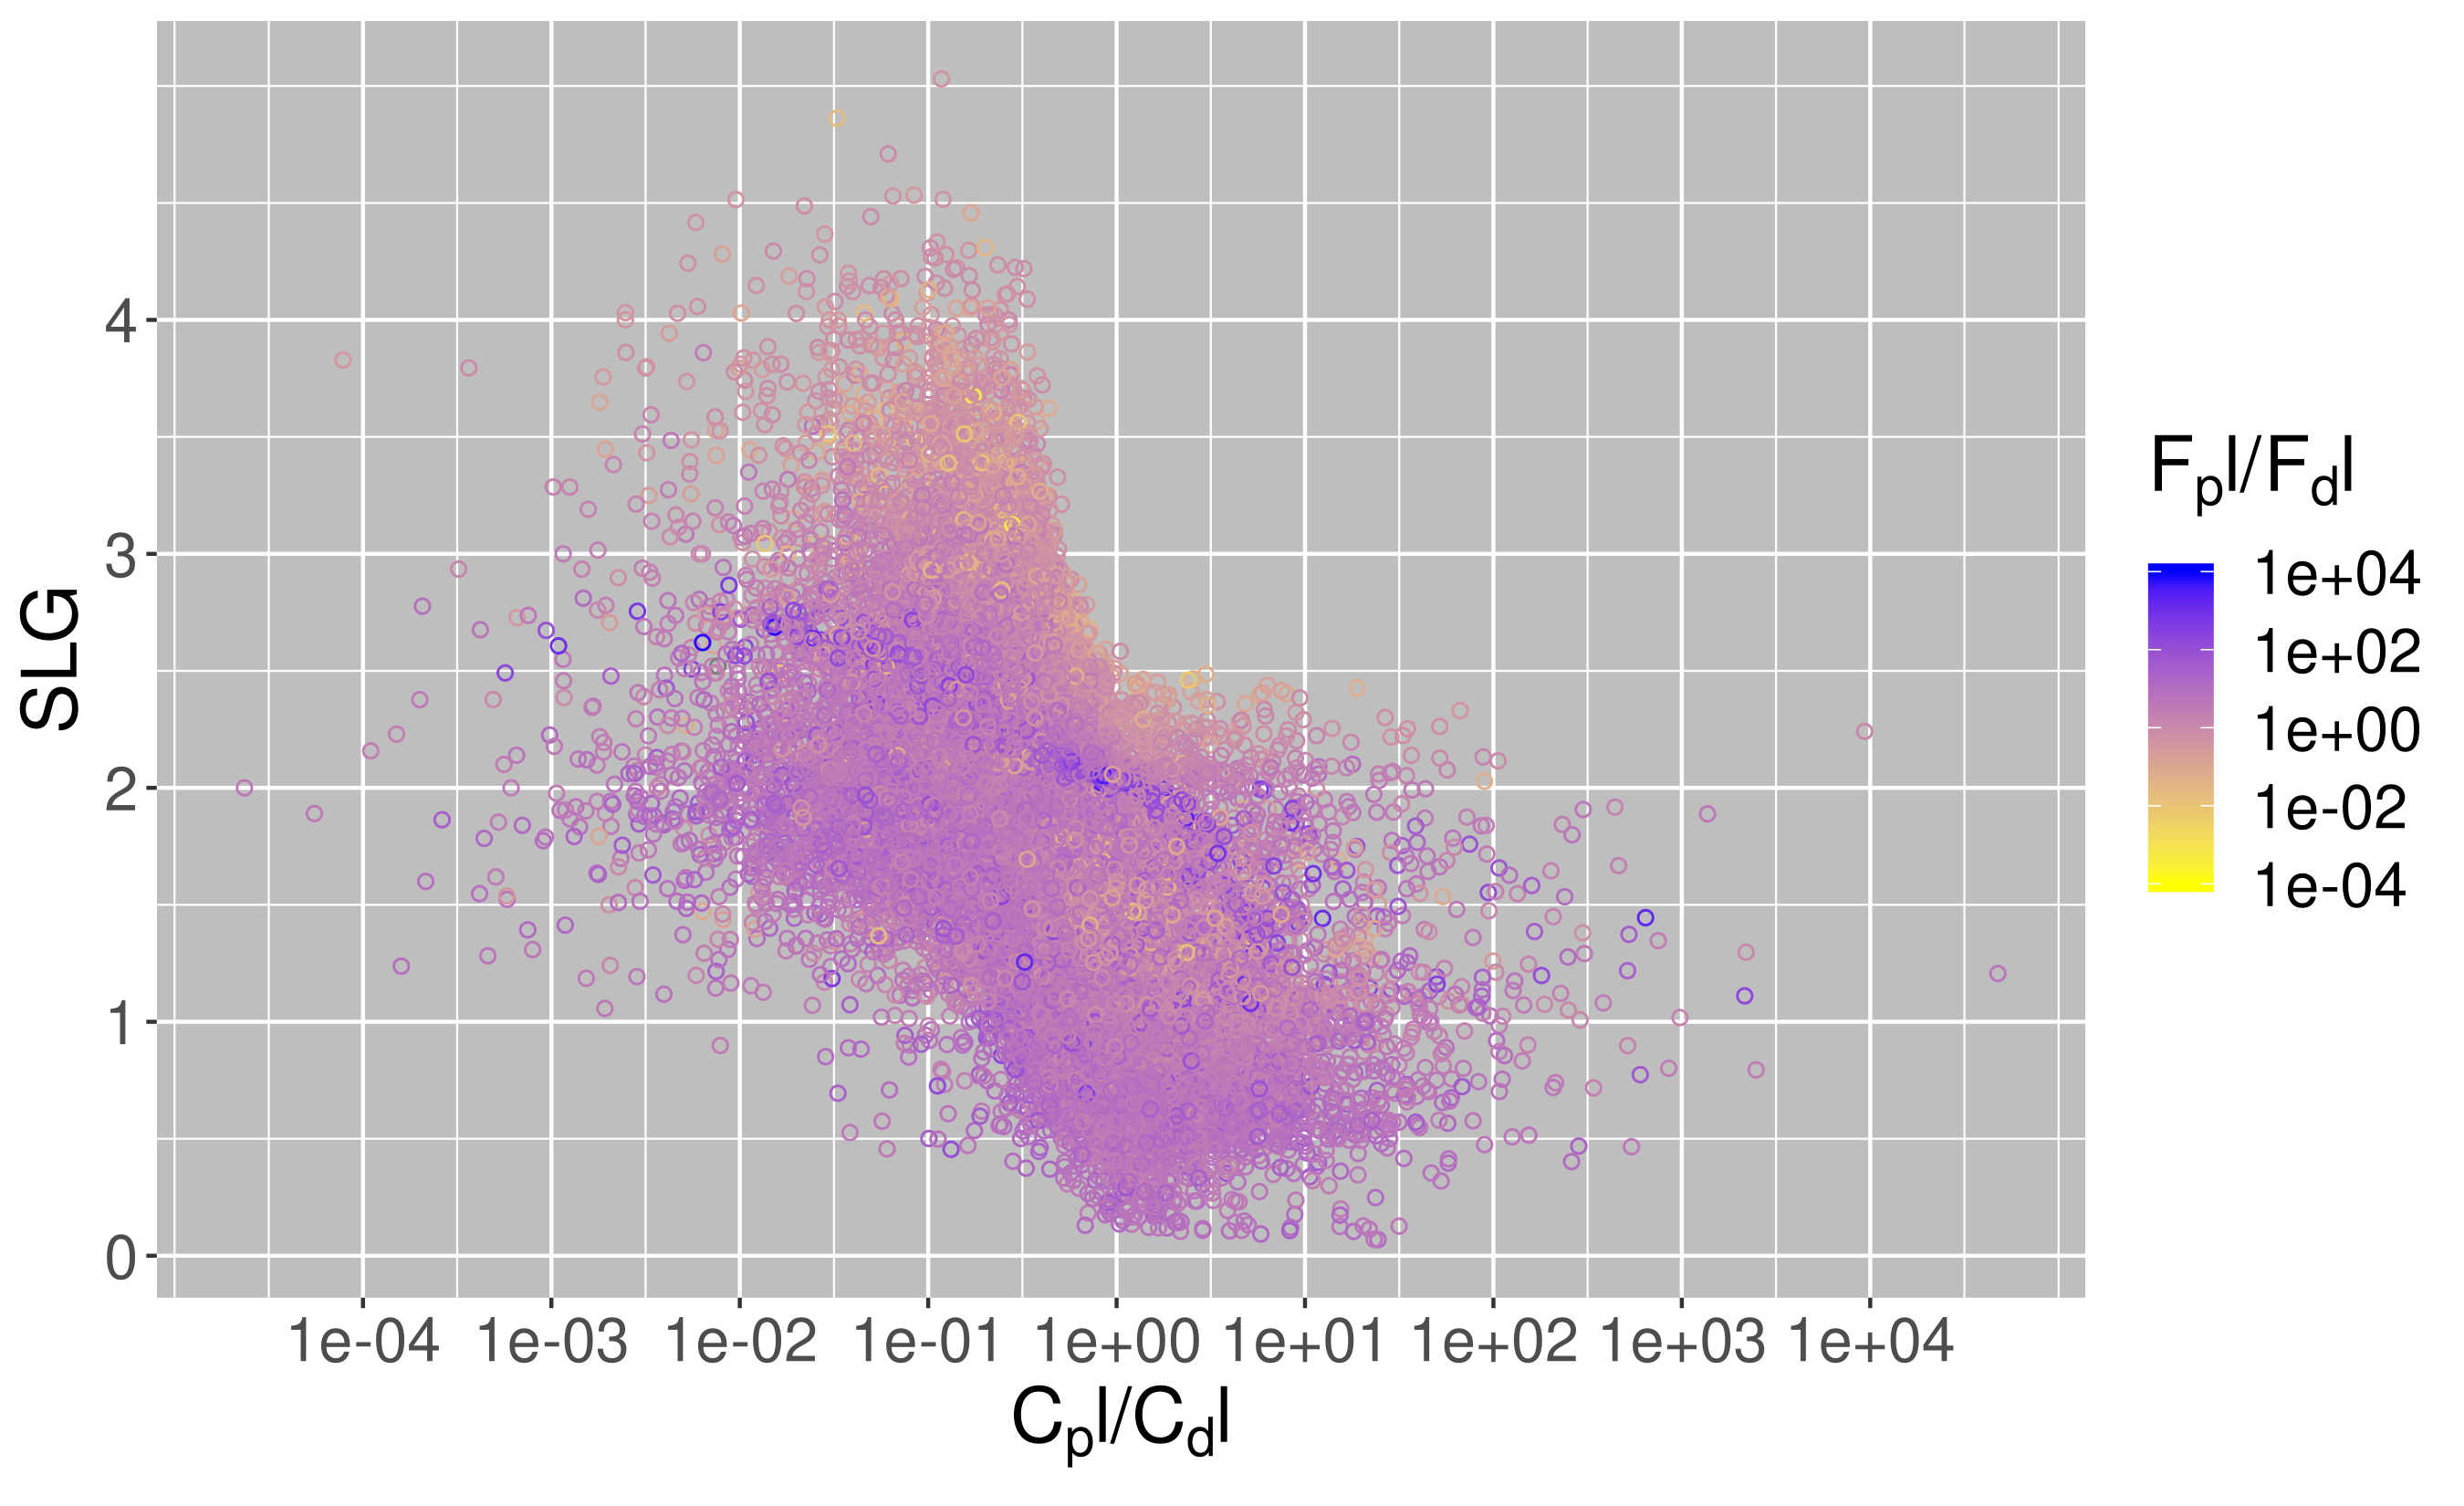
\includegraphics[width=5in]{/home/akara/workspace/R/CHAAHK/REPLACEME/figures/5-30}
	Plot corresponding to Figure 5.30 of Kara 2018
	\label{fig:5-30}
\end{figure}
\begin{thebibliography}{9}
	\bibitem{kara2018a}
	Kara, Alex. ``CHAAHK: a Spatial Simulation of the Maya Elevated Core Region'' (Version 1.0.0). CoMSES Computational Model Library, 2018. https://www.comses.net/codebases/b9335c92-f29e-42cf-aac8-712f6c587aad/releases/1.0.0/
	\bibitem{kara2018b}
	Kara, Alex. CHAAHK: A Spatial Simulation Model of the Maya Elevated Core Region. Diss. University of Cincinnati, 2018.
\end{thebibliography}
\end{document}
